\bookpart{谱分析}{Spectral Analysis}
\label{part:spectral-analysis}

\BookPartGuide{%
第一部分把矩阵解释为线性映射在坐标下的记录，并说明同一个映射在不同基下有不同的矩阵。本部分研究怎样选基，才能把一个给定的线性作用看清楚，再用这些表示回答两个实际问题：数据带误差时结果有多可靠，同一个作用反复施加时最终会怎样。

前三章建立表示。谱分解一章让输入、输出共用一组基，寻找只被伸缩的方向；能用正交基对角化的恰好是对称矩阵，一般方阵只能化为实Schur形。奇异值分解一章让两端各取一组标准正交基，使任何矩阵都化为非负的对角伸缩，并由奇异值读出范数和秩。极分解一章把同一作用重新组合为对称伸缩与保长转向，并把开方、求逆等沿谱进行的运算归纳为矩阵函数。

后两章使用这些表示。条件数与谱扰动一章先固定矩阵，研究输入误差的放大，再让矩阵本身带误差，估计特征值、奇异值、秩与特征子空间的变化；所有结论都是有限扰动下的界。线性递推的收敛与稳定性一章研究固定更新的反复作用，由谱半径判断初值影响是否消失，由Neumann级数求出平衡，并分析暂时放大与逐步误差的累积。

阅读时要注意区分几组相近的概念：同一组基下的相似变换与两端分别换基；特征值与奇异值；谱半径描述的长期倍率与范数描述的一步放大；输入带误差与矩阵带误差；有限扰动界与沿指定方向的一阶响应。Rayleigh商以及低秩、正交逼近的最优性在第三部分的矩阵逼近一章讨论；一阶响应与局部条件数在第四部分借助微分讨论。}

\chapter{特征值与谱分解}
\label{chap:eigen-spectral-decomposition}
\label{chap:linear-analysis}
\label{chap:matrix-analysis}

第~\ref{chap:linear-representation}章说明，矩阵是线性映射在一组基下的坐标表示。对把空间映到自身的线性算子，输入和输出同时换成一组新基时，矩阵按相似关系$\bm B=\bm P^{-1}\bm A\bm P$改变（第~\ref{sec:ls-similarity}节），所以同一个作用有许多种矩阵写法。那里的例子中，算子$T(x_1,x_2)=(2x_1+x_2,3x_2)$在标准基下的矩阵有非零的非对角元，换到合适的基以后却成了对角矩阵：新基的两个方向在作用下只被伸缩，不被转向。

本章研究一般的表示问题：给定方阵，能否找到这样的方向？能找到多少？如果还要求新基保持长度和夹角，矩阵最多能化到多简单？这几个问题依次加强对基的要求，答案也依次收窄。

第~\ref{sec:ls-linear-operators}节寻找只被伸缩的方向，即特征向量，用特征多项式求出特征值，并说明它们不随基改变。第~\ref{sec:ls-matrix-powers}节判断特征向量何时多到足以组成一组基；这时矩阵相似于对角矩阵，矩阵幂化为特征值的乘方，但所用的特征基一般不正交。第~\ref{sec:ls-spectral-theory}节要求换基矩阵正交，证明能这样对角化的恰好是实对称矩阵，并把分解写成与基的选取无关的谱投影之和。第~\ref{sec:ls-general-square-spectrum}节处理一般方阵：允许复特征值以后，正交换基只能得到分块上三角的实Schur形，能化为分块对角形的恰好是正规矩阵。

本章用到第~\ref{chap:linear-operations}章的矩阵运算与行列式、第~\ref{chap:linear-representation}章的线性映射、换基与相似，以及第~\ref{chap:normed-inner-product-spaces}章的范数、内积、正交投影与正定矩阵。这里得到的谱定理是后面几章的共同工具：第~\ref{chap:singular-value-decomposition}章用它构造奇异值分解，第~\ref{chap:polar-decomposition}章用它开方，第~\ref{chap:condition-and-spectral-perturbation}章和第~\ref{chap:linear-recurrence-stability}章用特征值与谱半径分析扰动和反复作用。

% 第4章第1节：特征值与特征向量（特征方向、特征空间、特征多项式与Cayley--Hamilton定理、相似不变性、特征向量的线性无关性）。

\section{特征值与特征向量}
\label{sec:ls-linear-operators}

第~\ref{sec:ls-similarity}节的例子中，算子$T(x_1,x_2)=(2x_1+x_2,3x_2)$换到新基$\bm b_1'=\bm e_1$、$\bm b_2'=\bm e_1+\bm e_2$以后，矩阵成为对角矩阵$\operatorname{diag}(2,3)$，因为这两个基方向在作用下只被伸缩、不被转向。不过，那组基是事先给出、再加以验证的。

本节给出寻找这类方向的一般方法。特征向量的定义只说明要找什么；要系统地找出它们，需要把条件改写成特征多项式的根。求出的特征值还要与基无关，才是算子本身的性质；最后，不同特征值的特征向量线性无关，这为下一节用它们组成基作准备。

\subsection{线性作用中的特征方向}
\label{sec:ls-operator-eigenvectors}

第~\ref{sec:ls-linear-map-definition}节说明，线性算子$T:V\to V$总把原点留在原处，但一般会同时改变向量的长度和方向。我们要找的是这样的非零向量：作用以后仍落在原来那条过原点的直线上，只被伸长、缩短或反向。用等式表达，就是要求非零向量$\bm v\in V$与实数$\lambda$满足
\begin{equation}
T\bm v=\lambda\bm v,\qquad\bm v\neq\bm0.
\label{eq:matrix-analysis-eigenpair}
\end{equation}
这时称$\lambda$为$T$的\term{特征值}（eigenvalue），$\bm v$为属于$\lambda$的\term{特征向量}（eigenvector），$\bm v$所在的直线称为\term{特征方向}。

定义要求特征向量非零，因为零向量对任何$\lambda$都满足$T\bm0=\lambda\bm0$，不提供方向信息。特征值说明这条直线上发生了什么：$|\lambda|>1$时向量被拉长，$|\lambda|<1$时被缩短，$\lambda<0$时方向还被反过来；$\lambda=0$表示$T\bm v=\bm0$，即$\bm v$在$T$的核中。

在特征方向上，反复作用也最简单。第~\ref{sec:ls-operator-powers}节说明，算子可以与自身复合，得到$T^k$。对特征向量$\bm v$，由$T\bm v=\lambda\bm v$与线性性得$T^2\bm v=T(\lambda\bm v)=\lambda T\bm v=\lambda^2\bm v$，归纳即得$T^k\bm v=\lambda^k\bm v$。所以在这条直线上，$k$次作用化为数$\lambda$的$k$次乘方。

特征值是算子本身的性质，不依赖基的选取。取一组基$\mathcal B$后，式~\eqref{eq:matrix-analysis-eigenpair}的坐标形式是$[T]_{\mathcal B}[\bm v]_{\mathcal B}=\lambda[\bm v]_{\mathcal B}$。等式两侧分别是向量$T\bm v$与$\lambda\bm v$的坐标，而$\bm v\neq\bm0$当且仅当它的坐标非零。所以无论取哪组基，矩阵$[T]_{\mathcal B}$的特征值都恰好是$T$的特征值；换基只改变特征向量的坐标。

反过来，方阵也可以看作算子。对$n$阶方阵$\bm A$，它的特征值与特征向量指算子$\bm x\mapsto\bm A\bm x$的特征值与特征向量，即满足$\bm A\bm v=\lambda\bm v$、$\bm v\neq\bm0$的$\lambda$与$\bm v$。

回到开头的算子，可以逐个验证哪些方向是特征方向。
\begin{example}[验证特征向量]
\label{ex:ls-operator-eigenvector-check}
算子$T(x_1,x_2)=(2x_1+x_2,3x_2)$在标准基下的矩阵为
\[
 \bm A=\begin{bmatrix}2&1\\0&3\end{bmatrix}.
\]
我们看$\bm e_1$、$(1,1)^{\top}$与$\bm e_2$三个向量中哪些是特征向量。按定义，只需把每个向量乘以$\bm A$，看结果是否仍是原向量的倍数：
\[
\begin{gathered}
\bm A\bm e_1=\begin{bmatrix}2\\0\end{bmatrix}=2\bm e_1\\
\bm A\begin{bmatrix}1\\1\end{bmatrix}=\begin{bmatrix}3\\3\end{bmatrix}=3\begin{bmatrix}1\\1\end{bmatrix}\\
\bm A\bm e_2=\begin{bmatrix}1\\3\end{bmatrix}.
\end{gathered}
\]
前两个向量只被分别乘以$2$和$3$，所以$\bm e_1$与$(1,1)^{\top}$是特征向量，特征值分别为$2$和$3$；它们正是第~\ref{sec:ls-similarity}节新基的两个方向，这就解释了那组基为什么能把矩阵化成$\operatorname{diag}(2,3)$。$\bm e_2$则被送到$(1,3)^{\top}$，这不是$\bm e_2$的倍数，所以$\bm e_2$不是特征向量。
\end{example}
图~\ref{fig:ls-operator-eigenvectors}画出这个例子：两条特征方向上的向量作用后仍在原直线上，只是变长；其他方向上的向量被转开。
\begin{figure}[!htb]
  \centering
  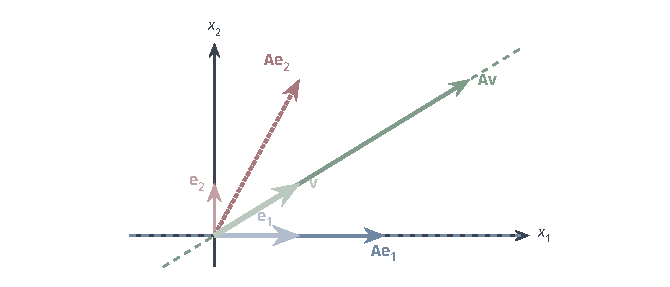
\includegraphics[width=112mm]{figures/00-shared/mathematical-preliminaries-upper/02-linear-spaces/tikz/comprehension-additions/operator-eigenvectors.pdf}
  \caption{特征向量只被伸缩、不被转向。算子$T(x_1,x_2)=(2x_1+x_2,3x_2)$在标准基下的矩阵为$\bm A=\left[\begin{smallmatrix}2&1\\0&3\end{smallmatrix}\right]$，它把$\bm e_1$送到$2\bm e_1$，把$\bm v=(1,1)^{\top}$送到$3\bm v$，二者都留在各自的虚线上；$\bm e_2$被送到$(1,3)^{\top}$，偏离了原来的直线，所以不是特征向量。}
  \label{fig:ls-operator-eigenvectors}
\end{figure}

并非每个算子都有实特征向量。下面的反例中，每个非零向量都被转离原来的直线。
\begin{example}[反例：平面旋转没有实特征向量]
\label{ex:ls-rotation-no-real-eigenvector}
考虑平面上逆时针旋转$90^\circ$的算子$R(x_1,x_2)=(-x_2,x_1)$。直观上，每个非零向量都被转过直角，不可能留在原来的直线上；下面用方程确认这一点。设实数$\lambda$与向量$(x_1,x_2)$满足$R(x_1,x_2)=\lambda(x_1,x_2)$，按分量写出就是
\[
 \begin{gathered}
-x_2=\lambda x_1\\
x_1=\lambda x_2 .
 \end{gathered}
\]
把第二式代入第一式得$-x_2=\lambda^2x_2$，即$(1+\lambda^2)x_2=0$。由于$1+\lambda^2>0$，只能$x_2=0$，进而$x_1=\lambda x_2=0$。可见无论取哪个实数$\lambda$，满足等式的都只有零向量，所以$R$既没有实特征值，也没有实特征向量。
\end{example}

\subsection{特征空间与不变子空间}

同一个特征值可以对应不止一条特征方向，所以应把它们放在一起考察。固定特征值$\lambda$，满足$T\bm v=\lambda\bm v$的全部向量连同零向量组成集合$\ker(T-\lambda\,\operatorname{id}_V)$，称为$\lambda$的\term{特征空间}（eigenspace）。它是一个线性映射的核，因而是子空间。

例如$\bm I_2$的每个非零向量都是属于$1$的特征向量，特征空间是整个平面；而示例~\ref{ex:ls-operator-eigenvector-check}中属于$2$的特征空间只是$\bm e_1$所在的直线，因为$\bm A-2\bm I=\left[\begin{smallmatrix}0&1\\0&1\end{smallmatrix}\right]$的核由第二坐标为零的向量组成。

特征空间是一类更一般的子空间的特例。若子空间$S$满足$T(S)\subseteq S$，就称$S$为$T$的\term{不变子空间}（invariant subspace）。这时作用不会把$S$中的向量带出$S$，可以把$T$限制在$S$上单独研究。特征空间中的向量只被乘以$\lambda$，仍留在其中，所以特征空间是不变子空间。

一维不变子空间恰好就是特征方向。若$\bm v\neq\bm0$且$\operatorname{span}\{\bm v\}$不变，则$T\bm v$落在这条直线上，是$\bm v$的倍数；反之，若$T\bm v=\lambda\bm v$，则$T(c\bm v)=\lambda c\bm v$仍在这条直线上。高于一维的不变子空间却未必含有特征方向：整个平面对$90^\circ$旋转不变，而示例~\ref{ex:ls-rotation-no-real-eigenvector}说明其中没有一条特征方向。这样的二维不变子空间对应一对共轭的复特征值（第~\ref{sec:ls-general-square-spectrum}节）。

\subsection{特征多项式}
\label{sec:ls-characteristic-polynomial}

示例~\ref{ex:ls-operator-eigenvector-check}中的特征向量是先猜出、再验证的。要系统地求出全部特征值，可以把特征值的条件改写成矩阵不可逆。对$n$阶方阵$\bm A$，$\lambda$是特征值，当且仅当齐次方程$(\bm A-\lambda\bm I)\bm v=\bm0$有非零解，即$\ker(\bm A-\lambda\bm I)\neq\{\bm0\}$。由第~\ref{sec:ls-injective-surjective-invertible}节的等价条件，这又等价于$\operatorname{rank}(\bm A-\lambda\bm I)<n$，也等价于$\bm A-\lambda\bm I$不可逆。

不可逆又等价于行列式为零，这一步用到第~\ref{sec:ls-determinant-properties}节的两条性质。若方阵$\bm M$可逆，乘法性给出$\det\bm M\det(\bm M^{-1})=\det\bm I=1$，故$\det\bm M\neq0$；反之若$\det\bm M\neq0$，古典伴随恒等式说明$\operatorname{adj}(\bm M)/\det\bm M$就是$\bm M$的逆。所以$\lambda$是$\bm A$的特征值，当且仅当$\det(\bm A-\lambda\bm I)=0$。

这也解释了第~\ref{sec:ls-similarity-properties}节的一个相似不变量。那里把每个$\operatorname{rank}(\bm A-c\bm I)$都列为相似不变量；现在可以看出，使这个秩小于$n$的数$c$恰好就是特征值。

把这个条件写成首项系数为$1$的多项式更方便。由于$\det(\lambda\bm I-\bm A)=(-1)^n\det(\bm A-\lambda\bm I)$，二者同时为零。定义
\begin{equation}
 p_{\bm A}(z)=\det(z\bm I-\bm A),
 \label{eq:matrix-analysis-characteristic-polynomial}
\end{equation}
称为\term{特征多项式}（characteristic polynomial），就得到：$\bm A$的实特征值恰为$p_{\bm A}$的实根。

再看$p_{\bm A}$的次数。在行列式的排列展开中，对角线一项是$\prod_i(z-a_{i,i})$；其余每一项至少有两个因子取自非对角位置，含$z$的因子至多$n-2$个。所以只有对角线一项含$z^n$，$p_{\bm A}$是首项系数为$1$的$n$次实多项式，至多有$n$个不同的根。求出一个特征值$\lambda$以后，再解齐次方程$(\bm A-\lambda\bm I)\bm v=\bm0$，就得到它的特征空间。

用特征多项式可以重新求出前面两个例子的特征值，不必再猜测特征向量。
\begin{example}[用特征多项式求特征值]
\label{ex:ls-characteristic-polynomial-two-by-two}
回到示例~\ref{ex:ls-operator-eigenvector-check}的矩阵$\bm A$，以及示例~\ref{ex:ls-rotation-no-real-eigenvector}中旋转在标准基下的矩阵$\bm R$：
\[
 \bm A=\begin{bmatrix}2&1\\0&3\end{bmatrix},\qquad
 \bm R=\begin{bmatrix}0&-1\\1&0\end{bmatrix}.
\]
这一次不猜特征向量，而是直接计算$\det(z\bm I-\bm A)$与$\det(z\bm I-\bm R)$：
\[
 \begin{aligned}
 p_{\bm A}(z)&=\det\begin{bmatrix}z-2&-1\\0&z-3\end{bmatrix}=(z-2)(z-3),\\
 p_{\bm R}(z)&=\det\begin{bmatrix}z&1\\-1&z\end{bmatrix}=z^2+1 .
 \end{aligned}
\]
$p_{\bm A}$的两个根$2$与$3$正是示例~\ref{ex:ls-operator-eigenvector-check}中两条特征方向上的伸缩倍数，而且这里不需要事先知道那两条方向。$z^2+1$对任何实数$z$都为正，没有实根，所以$\bm R$没有实特征值，与示例~\ref{ex:ls-rotation-no-real-eigenvector}直接解方程的结论一致。
\end{example}
$\bm A$的情形可以推广到任意三角矩阵：三角矩阵$\bm A$的$z\bm I-\bm A$仍是三角矩阵，行列式是对角元之积$\prod_i(z-a_{i,i})$，所以三角矩阵的特征值就是它的对角元。

特征多项式在每个特征值处取零。把矩阵本身代入特征多项式，结果是零矩阵。这里的代入是指把多项式中的$z^j$换成$\bm A^j$，常数项$c_0$换成$c_0\bm I$。先在一个例子中验证。
\begin{example}[把矩阵代入它的特征多项式]
\label{ex:ls-cayley-hamilton-two-by-two}
仍取
\[
 \bm A=\begin{bmatrix}2&1\\0&3\end{bmatrix}.
\]
由示例~\ref{ex:ls-characteristic-polynomial-two-by-two}，$p_{\bm A}(z)=(z-2)(z-3)=z^2-5z+6$。把$z^2$换成$\bm A^2$、$z$换成$\bm A$、常数$6$换成$6\bm I$，需要先算出$\bm A^2$，再逐个元素合并：
\[
\begin{gathered}
\bm A^2=\begin{bmatrix}4&5\\0&9\end{bmatrix}\\
\bm A^2-5\bm A+6\bm I
 =\begin{bmatrix}4-10+6&5-5+0\\0&9-15+6\end{bmatrix}
 =\bm0 .
\end{gathered}
\]
四个元素全部抵消，$p_{\bm A}(\bm A)$是零矩阵。两个对角元分别是$p_{\bm A}(2)$与$p_{\bm A}(3)$，为零是因为$2,3$是特征值；右上角的抵消则来自$\bm A^2$与$5\bm A$的非对角元恰好相等，单看特征值处取零并不能预见。
\end{example}
这一结论对每个方阵都成立。
\begin{theorem}[Cayley--Hamilton定理]
\label{thm:ls-cayley-hamilton}
设$n$阶方阵$\bm A$的特征多项式为$p_{\bm A}(z)=z^n+c_{n-1}z^{n-1}+\cdots+c_0$，则
\[
 p_{\bm A}(\bm A)
 =\bm A^n+c_{n-1}\bm A^{n-1}+\cdots+c_1\bm A+c_0\bm I=\bm0.
\]
\end{theorem}
\begin{proof}
证明的工具是第~\ref{sec:ls-det-cofactor-adjugate}节的古典伴随恒等式（定理~\ref{thm:ls-adjugate-identity}）$\bm M\operatorname{adj}(\bm M)=\det(\bm M)\bm I$。令$\bm M=z\bm I-\bm A$，得
\[
 (z\bm I-\bm A)\operatorname{adj}(z\bm I-\bm A)=p_{\bm A}(z)\bm I .
\]
$\operatorname{adj}(z\bm I-\bm A)$的每个元素都是$z\bm I-\bm A$的一个带符号的$n-1$阶余子式，它是$z$的多项式，次数不超过$n-1$。按$z$的幂次整理，可以写成$\operatorname{adj}(z\bm I-\bm A)=\sum_{j=0}^{n-1}z^j\bm B_j$，其中$\bm B_j$是不含$z$的常数矩阵。

代入上式，左边为$\sum_jz^{j+1}\bm B_j-\sum_jz^j\bm A\bm B_j$。两边每个元素都是$z$的多项式，且对所有实数$z$相等，所以同次项的系数相等。记$c_n=1$，比较$z$的各次幂系数：
\[
 \begin{aligned}
 &z^n: &&\bm B_{n-1}=\bm I;\\
 &z^j\ (1\leq j\leq n-1): &&\bm B_{j-1}-\bm A\bm B_j=c_j\bm I;\\
 &z^0: &&-\bm A\bm B_0=c_0\bm I .
 \end{aligned}
\]
把$z^j$项的等式左乘$\bm A^j$（$j=0,\ldots,n$）后相加。右边恰为$\sum_jc_j\bm A^j=p_{\bm A}(\bm A)$；左边为
\[
 \bm A^n\bm B_{n-1}+\sum_{j=1}^{n-1}\bigl(\bm A^j\bm B_{j-1}-\bm A^{j+1}\bm B_j\bigr)-\bm A\bm B_0 ,
\]
其中相邻项逐对相消，总和为零。
\end{proof}
证明只用到行列式与古典伴随，既不需要先求出特征值，也不要求$p_{\bm A}$有实根。

由定理可以推出，矩阵的高次幂都能由低次幂表示。
\begin{theorem}[高次幂的降次]
\label{thm:ls-power-reduction}
设$\bm A$为$n$阶方阵，则对每个整数$k\geq0$，
\[
 \bm A^k\in\operatorname{span}\{\bm I,\bm A,\ldots,\bm A^{n-1}\}.
\]
因而对任意向量$\bm g$与$k\geq0$，
\[
 \bm A^k\bm g\in\operatorname{span}\{\bm g,\bm A\bm g,\ldots,\bm A^{n-1}\bm g\},
\]
前$k$项$\bm g,\ldots,\bm A^{k-1}\bm g$张成的子空间在$k\geq n$时不再增大。
\end{theorem}
\begin{proof}
记$\mathcal P=\operatorname{span}\{\bm I,\bm A,\ldots,\bm A^{n-1}\}$。$k<n$时结论显然。对$k\geq n$归纳。$k=n$时，由定理~\ref{thm:ls-cayley-hamilton}，
\[
 \bm A^n=-\sum_{j=0}^{n-1}c_j\bm A^j\in\mathcal P .
\]
设$\bm A^k=\sum_{j=0}^{n-1}d_j\bm A^j\in\mathcal P$。两边左乘$\bm A$，得
\[
 \bm A^{k+1}=\sum_{j=0}^{n-2}d_j\bm A^{j+1}+d_{n-1}\bm A^n .
\]
右端第一个和属于$\mathcal P$，$\bm A^n$也属于$\mathcal P$，所以$\bm A^{k+1}\in\mathcal P$。

对向量$\bm g$，把$\bm A^k=\sum_jd_j\bm A^j$作用于$\bm g$，即得$\bm A^k\bm g=\sum_{j=0}^{n-1}d_j\bm A^j\bm g$。于是$k\geq n$时新加入的向量$\bm A^{k-1}\bm g$已在前$n$个向量张成的子空间中，子空间不再增大。
\end{proof}
所以序列$\bm g,\bm A\bm g,\bm A^2\bm g,\ldots$张成的子空间至多是$n$维的，并且由前$n$项决定。第~\ref{chap:matrix-equations}章判断Sylvester方程何时有唯一解，第~\ref{chap:krylov-methods}章研究Krylov子空间方法时，都要用到这一点。

回到特征值本身。同一个特征值可以是特征多项式的重根，这时要区分两种“个数”。根$\lambda$在$p_{\bm A}$中的重数称为\term{代数重数}（algebraic multiplicity），特征空间的维数$\dim\ker(\bm A-\lambda\bm I)$称为\term{几何重数}（geometric multiplicity）。下面的例子说明二者可以不同。
\begin{example}[代数重数大于几何重数]
\label{ex:ls-multiplicity-gap}
取
\[
 \bm J=\begin{bmatrix}0.8&1\\0&0.8\end{bmatrix}.
\]
它是上三角矩阵，特征多项式为$p_{\bm J}(z)=(z-0.8)^2$，所以唯一的特征值$0.8$是二重根，代数重数为$2$。要知道几何重数，还得解出特征空间：
\[
\begin{gathered}
\bm J-0.8\bm I=\begin{bmatrix}0&1\\0&0\end{bmatrix}\\
(\bm J-0.8\bm I)\begin{bmatrix}x_1\\x_2\end{bmatrix}=\begin{bmatrix}x_2\\0\end{bmatrix},
\end{gathered}
\]
它为零当且仅当$x_2=0$，所以特征空间只是$(1,0)^{\top}$所在的直线，几何重数为$1$。特征多项式把$0.8$数了两次，特征方向却只有一条；右上角的$1$正是使第二条特征方向消失的原因。
\end{example}
两种重数的一般关系，以及它们怎样决定能否找到由特征向量组成的基，在第~\ref{sec:ls-matrix-powers}节讨论。对一般的算子$T$，可以取任一组基把它写成矩阵，再求特征多项式与两种重数。下一小节说明，结果不依赖基的选取。

\subsection{相似变换与谱的不变性}
\label{sec:ls-eigen-similarity-invariance}

第~\ref{sec:ls-similarity-properties}节列出了相似保持的量：秩、零空间的维数、每个$\operatorname{rank}(\bm A-c\bm I)$，以及行列式与迹。本小节说明，特征值、特征多项式与两种重数也是相似不变量，因此它们属于算子本身；再说明迹与行列式怎样由特征值读出，最后指出这些不变量只能否定相似。

\paragraph{特征值、特征空间与特征多项式}
下面的定理把这些不变性一并写出。

\begin{theorem}[谱的相似不变性]
\label{thm:ls-spectrum-similarity-invariance}
设$\bm B=\bm P^{-1}\bm A\bm P$，$\bm P$可逆，则：
\begin{enumerate}
 \item $\bm A$与$\bm B$的特征值相同；若$\bm A\bm v=\lambda\bm v$，则$\bm B(\bm P^{-1}\bm v)=\lambda\bm P^{-1}\bm v$，且$\ker(\bm B-\lambda\bm I)=\bm P^{-1}\ker(\bm A-\lambda\bm I)$，所以每个特征值的几何重数相同；
 \item $p_{\bm B}=p_{\bm A}$，所以每个特征值的代数重数相同。
\end{enumerate}
\end{theorem}
\begin{proof}
第一条。若$\bm A\bm v=\lambda\bm v$且$\bm v\neq\bm0$，则
\[
 \bm B(\bm P^{-1}\bm v)=\bm P^{-1}\bm A\bm P\bm P^{-1}\bm v=\bm P^{-1}\bm A\bm v=\lambda\bm P^{-1}\bm v .
\]
$\bm P$可逆保证$\bm P^{-1}\bm v\neq\bm0$，所以$\lambda$也是$\bm B$的特征值；交换$\bm A,\bm B$的角色即得反向结论。同样的计算说明$\bm P^{-1}$把$\ker(\bm A-\lambda\bm I)$映入$\ker(\bm B-\lambda\bm I)$，交换角色可知$\bm P$把后者映入前者，所以$\ker(\bm B-\lambda\bm I)=\bm P^{-1}\ker(\bm A-\lambda\bm I)$。可逆矩阵把子空间映成同维数的子空间，所以几何重数相同。这一结论也可以由式~\eqref{eq:ls-similarity-shifted-rank}取$c=\lambda$、再用秩零度定理换成核的维数得到。

第二条。由$z\bm I=\bm P^{-1}(z\bm I)\bm P$与第~\ref{sec:ls-similarity-properties}节的恒等式$\det(\bm P^{-1}\bm M\bm P)=\det\bm M$，
\[
 p_{\bm B}(z)=\det(z\bm I-\bm P^{-1}\bm A\bm P)=\det\bigl(\bm P^{-1}(z\bm I-\bm A)\bm P\bigr)=p_{\bm A}(z).
\]
\end{proof}
所以算子的特征值、特征多项式与两种重数都可以用任意一组基下的矩阵计算。

\paragraph{特征多项式的系数}
行列式与迹也是相似不变量，这可以由定理~\ref{thm:ls-spectrum-similarity-invariance}解释：它们就是$p_{\bm A}$的两个系数，至多差一个符号。
\begin{theorem}[迹、行列式与特征值]
\label{thm:ls-trace-det-eigenvalues}
设$\bm A$为$n$阶方阵，则
\[
 p_{\bm A}(z)=z^n-(\operatorname{tr}\bm A)\,z^{n-1}+\cdots+(-1)^n\det\bm A .
\]
若$p_{\bm A}(z)=\prod_{i=1}^n(z-\lambda_i)$分解为实一次因子之积，其中每个特征值按代数重数重复列出，则
\[
 \operatorname{tr}\bm A=\sum_{i=1}^n\lambda_i,\qquad\det\bm A=\prod_{i=1}^n\lambda_i .
\]
\end{theorem}
\begin{proof}
令$z=0$，得常数项$p_{\bm A}(0)=\det(-\bm A)=(-1)^n\det\bm A$。再看$z^{n-1}$的系数。第~\ref{sec:ls-characteristic-polynomial}节已经指出，排列展开中除对角线一项外，每一项含$z$的因子至多$n-2$个；所以$z^{n-1}$只来自$\prod_i(z-a_{i,i})$，系数为$-\sum_ia_{i,i}=-\operatorname{tr}\bm A$。若$p_{\bm A}=\prod_i(z-\lambda_i)$，展开右端，$z^{n-1}$的系数为$-\sum_i\lambda_i$，常数项为$(-1)^n\prod_i\lambda_i$，与上面比较即得两个等式。
\end{proof}
例如示例~\ref{ex:ls-operator-eigenvector-check}的$\bm A$有$\operatorname{tr}\bm A=5=2+3$，$\det\bm A=6=2\cdot3$。第~\ref{sec:ls-general-square-spectrum}节把特征多项式的复根也算作特征值以后，这两个等式对每个方阵都成立。

\paragraph{相似不变量只能否定相似}
相似不变量只能用来否定相似：某个相似不变量不同，两个矩阵就不相似；不变量全部相同，两个矩阵却未必相似。第~\ref{sec:ls-similarity-conditions}节比较过$\bm I_2$与$\left[\begin{smallmatrix}1&1\\0&1\end{smallmatrix}\right]$，下面用特征值的语言重新说明二者为什么不相似。
\begin{example}[反例：特征多项式相同而不相似]
\label{ex:ls-same-charpoly-not-similar}
比较$\bm I_2$与
\[
 \bm J_1=\begin{bmatrix}1&1\\0&1\end{bmatrix}.
\]
二者都是上三角矩阵，对角元都是$1$，所以$p_{\bm I_2}(z)=p_{\bm J_1}(z)=(z-1)^2$，特征值$1$的代数重数都是$2$。仅凭特征多项式无法把它们区分开，于是转而比较特征空间：
\[
\begin{gathered}
\bm I_2-\bm I_2=\bm0\\
\bm J_1-\bm I_2=\begin{bmatrix}0&1\\0&0\end{bmatrix},
\end{gathered}
\]
前者的核是整个平面，后者的核只是$(1,0)^{\top}$所在的直线，几何重数分别为$2$与$1$。由定理~\ref{thm:ls-spectrum-similarity-invariance}，相似矩阵的几何重数必须相同，所以二者不相似，尽管它们的特征多项式完全一样。
\end{example}
所以特征多项式相同只是相似的必要条件。比较各特征值的几何重数是更细的必要条件，但一般仍不足以判定相似；完整的相似分类需要Jordan标准形，本书不展开。

\subsection{特征向量的线性无关性}
\label{sec:ls-eigenvector-independence}

要用特征方向组成一组基，先要知道不同特征值的特征向量彼此不会重复。本小节先证明它们线性无关，再推出各特征空间之和是直和。

\paragraph{特征向量的线性无关}
设想两条特征方向属于不同的特征值。若其中一条落在另一条上，同一个向量就会被乘以两个不同的倍数，这不可能。下面的定理把这一观察推广到任意多个特征值。
\begin{theorem}[不同特征值的特征向量线性无关]
\label{thm:ls-distinct-eigenvectors-independent}
设$\bm v_1,\ldots,\bm v_r$分别是$T$属于互不相同的特征值$\lambda_1,\ldots,\lambda_r$的特征向量，则$\bm v_1,\ldots,\bm v_r$线性无关。特别地，$n$维空间上的算子至多有$n$个不同的特征值。
\end{theorem}
\begin{proof}
假设它们线性相关。在所有非平凡的线性依赖中取项数最少的一个，重新编号后记为$\sum_{j=1}^s c_j\bm v_j=\bm0$，其中各$c_j\neq0$；单个特征向量非零，不能单独构成依赖，所以$s\geq2$。两边作用$T-\lambda_1\operatorname{id}_V$：第一项变为零，其余各项变为$c_j(\lambda_j-\lambda_1)\bm v_j$。特征值互不相同，这些系数仍非零，于是得到一个只有$s-1$项的非平凡依赖，与$s$最少矛盾。$n$维空间中线性无关的向量至多$n$个，所以不同特征值至多$n$个。
\end{proof}
这一上界与特征多项式的次数给出的上界一致。

\paragraph{特征空间的直和}
同一个特征值可以有多维的特征空间。从每个特征空间各取一组基，合在一起是否仍线性无关？下面的定理给出肯定回答。
\begin{theorem}[特征空间之和是直和]
\label{thm:ls-eigenspaces-direct-sum}
设$\lambda_1,\ldots,\lambda_r$是$T$的互不相同的特征值，$E_i=\ker(T-\lambda_i\operatorname{id}_V)$。则和$E_1+\cdots+E_r$是直和；把各$E_i$的基合在一起，仍线性无关，因而$\dim(E_1+\cdots+E_r)=\sum_i\dim E_i$。
\end{theorem}
\begin{proof}
设$\bm w_1+\cdots+\bm w_r=\bm0$，$\bm w_i\in E_i$。其中非零的$\bm w_i$是属于不同特征值的特征向量，由定理~\ref{thm:ls-distinct-eigenvectors-independent}线性无关，不能相加为零，所以每个$\bm w_i=\bm0$，和是直和。把各$E_i$的基合在一起，它们的任一线性组合都可以按特征值分组写成$\sum_i\bm w_i$；若组合为零，则每个$\bm w_i=\bm0$，而每组基本身线性无关，所以全部系数为零。
\end{proof}

例如示例~\ref{ex:ls-operator-eigenvector-check}中的$\bm e_1$与$(1,1)^{\top}$属于不同的特征值$2$与$3$，不必另行验证，它们自动线性无关，在平面上组成一组基。

回顾本节：被算子只伸缩的方向是特征方向，伸缩倍数是特征值。特征值是特征多项式的实根，求出特征值后解齐次方程即得特征空间。特征值、特征多项式和两种重数都不随基改变，属于算子本身。

属于不同特征值的特征向量线性无关，所以$n$维空间上的算子至多有$n$个不同特征值。此外，Cayley--Hamilton定理说明$p_{\bm A}(\bm A)=\bm0$，由此$\bm A$的高次幂都能用$\bm I,\bm A,\ldots,\bm A^{n-1}$表示（定理~\ref{thm:ls-power-reduction}）。特征向量什么时候多到足以组成一组基，是下一节的对角化问题。

% 第4章第2节：对角化（特征基下的矩阵与幂、可对角化的判别及不能对角化的情形、计算步骤与算例）。

\section{对角化}
\label{sec:ls-matrix-powers}
\label{sec:ch06-powers-spectrum}

上一节找到了被算子只伸缩的方向，并证明属于不同特征值的特征向量线性无关。本节考察这些方向足以组成一组基的情形。先看这时矩阵和矩阵幂变成什么样，由此明白这种基为什么值得寻找；再给出它存在的条件，最后整理计算步骤。

本节的换基矩阵只要求可逆，各列不必互相垂直；要求正交换基的情形留给下一节。

\subsection{特征向量基下的矩阵表示}
\label{sec:matrix-analysis-spectrum}

设$\bm v_1,\ldots,\bm v_n$是由算子$T$的特征向量组成的基，$T\bm v_j=\lambda_j\bm v_j$。按第~\ref{sec:ls-map-representation}节的约定，$T$在这组基下的矩阵的第$j$列是$T\bm v_j=\lambda_j\bm v_j$的坐标，即第$j$个位置为$\lambda_j$、其余位置为零。所以这个矩阵在主对角线以外全为零，每个基方向被独立地伸缩。

示例~\ref{ex:ls-operator-eigenvector-check}中的$(\bm e_1,(1,1)^{\top})$就是这样一组基。换到这组基，正是第~\ref{sec:ls-similarity}节的相似变换$\bm P^{-1}\bm A\bm P=\operatorname{diag}(2,3)$；在图~\ref{fig:ls-similarity-change-of-basis-flow}中，基向量围成的平行四边形只沿两条特征方向分别伸长$2$倍和$3$倍。

这一观察可以写成矩阵等式。设$\bm A$是$T$在标准基下的矩阵，把特征向量的标准坐标排成$\bm V=[\bm v_1,\ldots,\bm v_n]$。$\bm V$的各列是新基向量的旧坐标，所以它正是第~\ref{sec:ls-similarity}节的换基矩阵；各列线性无关，所以$\bm V$可逆（第~\ref{sec:ls-injective-surjective-invertible}节）。

再比较$\bm A\bm V$与$\bm V\bm\Lambda$。按乘积的列读法，$\bm A\bm V$的第$j$列是$\bm A\bm v_j=\lambda_j\bm v_j$；右乘对角矩阵$\bm\Lambda=\operatorname{diag}(\lambda_1,\ldots,\lambda_n)$把第$j$列乘以$\lambda_j$，所以$\bm V\bm\Lambda$的第$j$列也是$\lambda_j\bm v_j$。于是$\bm A\bm V=\bm V\bm\Lambda$，两边左乘或右乘$\bm V^{-1}$，即得
\[
 \begin{gathered}
\bm V^{-1}\bm A\bm V=\bm\Lambda\\
\bm A=\bm V\bm\Lambda\bm V^{-1}.
 \end{gathered}
\]

对角形式的好处在反复作用时最明显。定常迭代$\bm x^{(k+1)}=\bm A\bm x^{(k)}$走$k$步后得到$\bm x^{(k)}=\bm A^k\bm x^{(0)}$。第~\ref{sec:ls-matrix-power-rules}节规定了矩阵幂的写法，但直接连乘会不断混合各个坐标，看不出$\bm A^k$在$k$很大时是什么样子。把$\bm A=\bm V\bm\Lambda\bm V^{-1}$连乘$k$次，相邻的$\bm V^{-1}\bm V$相消（这就是式~\eqref{eq:ls-similarity-product}后面的$\bm B^k=\bm P^{-1}\bm A^k\bm P$），得到
\begin{equation}
\begin{gathered}
\bm A^k=\bm V\bm\Lambda^k\bm V^{-1}\\
\bm\Lambda^k=\operatorname{diag}(\lambda_1^k,\ldots,\lambda_n^k).
\end{gathered}
\label{eq:ls-diagonalization-power}
\end{equation}
于是求幂只需对对角元逐个乘方。

三个因子可以从右向左读：$\bm V^{-1}\bm x^{(0)}$给出初值在各特征方向上的坐标，$\bm\Lambda^k$把第$j$个坐标乘以$\lambda_j^k$，$\bm V$再把结果合回标准坐标。上一节已经看到，沿特征方向有$\bm A^k\bm v=\lambda^k\bm v$；式~\eqref{eq:ls-diagonalization-power}把这一点推广到任意初值。

下面用一个上三角矩阵演示这种计算。先把一个初值拆成特征方向上的分量，再对所有初值一并写出矩阵幂。
\begin{example}[用特征向量计算矩阵幂]
\label{ex:ls-triangular-power}
给定
\[
 \bm A=\begin{bmatrix}0.8&4\\0&0.5\end{bmatrix},
\]
计算$\bm A^k$。

第一步，求特征值与特征向量。$\bm A$是上三角矩阵，特征值为对角元$0.8$与$0.5$。直接验证
\[
\begin{gathered}
\bm A\begin{bmatrix}1\\0\end{bmatrix}=0.8\begin{bmatrix}1\\0\end{bmatrix}\\
\bm A\begin{bmatrix}-40/3\\1\end{bmatrix}
 =\begin{bmatrix}-32/3+4\\0.5\end{bmatrix}
 =0.5\begin{bmatrix}-40/3\\1\end{bmatrix},
\end{gathered}
\]
所以$\bm v_1=(1,0)^{\top}$与$\bm v_2=(-40/3,1)^{\top}$是特征向量。

第二步，计算一条轨迹。初值$(0,1)^{\top}$不在特征方向上，先把它拆成$(0,1)^{\top}=\tfrac{40}{3}\bm v_1+\bm v_2$。两个分量每作用一次分别乘以$0.8$与$0.5$，由线性性，
\[
 \bm A^k\begin{bmatrix}0\\1\end{bmatrix}
 =\frac{40}{3}\,0.8^k\bm v_1+0.5^k\bm v_2
 =\begin{bmatrix}\tfrac{40}{3}(0.8^k-0.5^k)\\0.5^k\end{bmatrix}.
\]
$k=1$时得$(4,0.5)^{\top}$，与直接计算$\bm A(0,1)^{\top}$一致。

第三步，对所有初值一并计算，即应用式~\eqref{eq:ls-diagonalization-power}。取
\[
 \bm V=\begin{bmatrix}1&-\tfrac{40}{3}\\0&1\end{bmatrix},\qquad
 \bm V^{-1}=\begin{bmatrix}1&\tfrac{40}{3}\\0&1\end{bmatrix},
\]
则
\[
 \bm A^k=\bm V\begin{bmatrix}0.8^k&0\\0&0.5^k\end{bmatrix}\bm V^{-1}
 =\begin{bmatrix}0.8^k&\tfrac{40}{3}(0.8^k-0.5^k)\\0&0.5^k\end{bmatrix}.
\]
结论：$\bm A^k$的第二列正是第二步的轨迹；整个迭代拆成两个独立的数列，分别按$0.8^k$与$0.5^k$衰减。
\end{example}
这种计算的前提是特征向量足以组成整个空间的一组基。下一小节讨论这个前提何时成立。

\subsection{可对角化的判别}

上一小节说明，有了由特征向量组成的基，$\bm A$就相似于一个对角矩阵。我们把相似于对角矩阵取作定义。
\begin{definition}[实可对角化]
\label{def:ls-real-diagonalizable}
设$\bm A$是$n$阶实方阵。若存在$n$阶实可逆矩阵$\bm V$与实对角矩阵$\bm\Lambda$使$\bm V^{-1}\bm A\bm V=\bm\Lambda$，即$\bm A$相似于实对角矩阵，就称$\bm A$\term{实可对角化}（diagonalizable over the reals）；求出这样的$\bm V$与$\bm\Lambda$，称为把$\bm A$对角化。
\end{definition}
“实”表示$\bm V$与$\bm\Lambda$的元素都是实数。本书在实数范围内讨论，下文所说的可对角化都指实可对角化。下面的判据把可对角化归结为特征向量是否足够多。
\begin{theorem}[对角化判据]
\label{thm:ls-diagonalization-criterion}
$n$阶实方阵$\bm A$实可对角化，当且仅当$\bm A$有$n$个线性无关的实特征向量。这时以这些特征向量为列组成$\bm V$，以相应特征值按同一顺序组成$\bm\Lambda=\operatorname{diag}(\lambda_1,\ldots,\lambda_n)$，就有$\bm V^{-1}\bm A\bm V=\bm\Lambda$。
\end{theorem}
\begin{proof}
设$\bm V$的各列为$\bm v_1,\ldots,\bm v_n$，$\bm\Lambda=\operatorname{diag}(\lambda_1,\ldots,\lambda_n)$。上一小节的列读法对任意这样的$\bm V$与$\bm\Lambda$都成立，它给出
\[
 \begin{gathered}
\bm A\bm V=\bm V\bm\Lambda
 \quad\Longleftrightarrow\quad
 \bm A\bm v_j=\lambda_j\bm v_j\\
j=1,\ldots,n.
 \end{gathered}
\]
若$\bm A$有$n$个线性无关的特征向量，以它们为列的$\bm V$可逆，左乘$\bm V^{-1}$即得$\bm V^{-1}\bm A\bm V=\bm\Lambda$。反过来，若$\bm V^{-1}\bm A\bm V=\bm\Lambda$，左乘$\bm V$得$\bm A\bm V=\bm V\bm\Lambda$，于是每列都满足$\bm A\bm v_j=\lambda_j\bm v_j$；$\bm V$可逆，所以各列线性无关，从而都非零，它们是$n$个线性无关的特征向量。
\end{proof}
由于属于不同特征值的特征向量线性无关（第~\ref{sec:ls-eigenvector-independence}节），判据给出一个常用的充分条件：$n$阶实方阵若有$n$个互不相同的实特征值，就实可对角化。示例~\ref{ex:ls-triangular-power}的矩阵即属此类。这个条件不是必要的：单位矩阵$\bm I_n$只有一个特征值$1$，本身却已经是对角矩阵。

\paragraph{不能对角化的矩阵}
判据要求$n$个线性无关的实特征向量，这一要求可能在两处落空。其一，实特征值不够。示例~\ref{ex:ls-rotation-no-real-eigenvector}与示例~\ref{ex:ls-characteristic-polynomial-two-by-two}已经说明，平面上的$90^\circ$旋转$\bm R=\left[\begin{smallmatrix}0&-1\\1&0\end{smallmatrix}\right]$没有实特征值，也就没有实特征向量，所以不能实对角化。

其二，实特征值有了，特征向量却不够。示例~\ref{ex:ls-multiplicity-gap}中的$\bm J=\left[\begin{smallmatrix}0.8&1\\0&0.8\end{smallmatrix}\right]$只有特征值$0.8$，而特征向量只有$(1,0)^{\top}$的倍数，凑不出两个线性无关的特征向量，所以$\bm J$也不能对角化。

对这样的矩阵，式~\eqref{eq:ls-diagonalization-power}不再可用，幂也不再是纯粹的乘方。下面直接计算$\bm J^k$来看这一点。
\begin{example}[不能对角化矩阵的幂]
\label{ex:ls-jordan-block-power}
给定
\[
 \bm J=\begin{bmatrix}0.8&1\\0&0.8\end{bmatrix},
\]
计算$\bm J^k$。把$\bm J$写成$0.8\bm I+\bm N$，其中
\[
\begin{gathered}
\bm N=\begin{bmatrix}0&1\\0&0\end{bmatrix}\\
\bm N^2=\bm0 .
\end{gathered}
\]
$0.8\bm I$与$\bm N$可交换，所以二项式展开成立；又因为$j\geq2$时$\bm N^j=\bm0$，展开后只剩前两项：
\[
 \bm J^k=(0.8\bm I+\bm N)^k=0.8^k\bm I+k\,0.8^{k-1}\bm N=\begin{bmatrix}0.8^k&k\,0.8^{k-1}\\0&0.8^k\end{bmatrix}.
\]
右上角相邻两项之比为$\dfrac{(k+1)\,0.8^{k}}{k\,0.8^{k-1}}=0.8\cdot\dfrac{k+1}{k}$，它在$k<4$时大于$1$，在$k>4$时小于$1$。结论：右上角的$k\,0.8^{k-1}$随$k$先增大、后衰减，不能由单个特征值的乘方描述。
\end{example}

\paragraph{重数判据}
两个反例的缺陷可以用重数说明。$\bm R$的特征多项式$z^2+1$不能分解为实一次因子；$\bm J$的特征多项式$(z-0.8)^2$分解了，但特征值$0.8$的几何重数$1$小于代数重数$2$。下面证明，这两种缺陷恰好是全部障碍。于是能否对角化可以直接由特征多项式和特征空间的维数判断，不必逐个尝试特征向量。

先比较两种重数。
\begin{theorem}[几何重数不超过代数重数]
\label{thm:ls-geometric-algebraic-multiplicity}
设$\lambda$是$n$阶方阵$\bm A$的特征值，几何重数为$g=\dim\ker(\bm A-\lambda\bm I)$，代数重数为$m$，则$1\leq g\leq m$。更确切地，$(z-\lambda)^g$整除$p_{\bm A}(z)$。
\end{theorem}
\begin{proof}
$\lambda$是特征值，特征空间非零，所以$g\geq1$。取特征空间的一组基$\bm v_1,\ldots,\bm v_g$，并扩充成全空间的一组基，以它们为列组成可逆矩阵$\bm P$。前$g$个基向量都被送到自身的$\lambda$倍，所以$\bm A\bm P$的前$g$列是$\lambda\bm v_1,\ldots,\lambda\bm v_g$，即$\bm P^{-1}\bm A\bm P$的前$g$列是$\lambda\bm e_1,\ldots,\lambda\bm e_g$。于是$\bm A$相似于分块上三角矩阵
\[
 \begin{bmatrix}\lambda\bm I_g&*\\\bm0&\bm C\end{bmatrix}.
\]
相似不改变特征多项式（第~\ref{sec:ls-eigen-similarity-invariance}节），所以可以用这个分块矩阵计算$p_{\bm A}$。用$z\bm I$减去它以后，前$g$列都只在对角位置上有非零元素$z-\lambda$。沿第一列按余子式展开（第~\ref{sec:ls-det-cofactor-adjugate}节），得到$z-\lambda$乘以一个形状相同、但只剩$g-1$个这种列的行列式；重复$g$次，即得$p_{\bm A}(z)=(z-\lambda)^g\,p_{\bm C}(z)$。所以$\lambda$作为$p_{\bm A}$的根，重数至少为$g$，即$m\geq g$。
\end{proof}
示例~\ref{ex:ls-multiplicity-gap}说明不等号可以严格成立：那里$g=1$而$m=2$。

有了这个不等式，就可以把对角化判据中“$n$个线性无关的特征向量”换成只涉及特征多项式和特征空间维数的条件。
\begin{theorem}[重数判据]
\label{thm:ls-diagonalization-multiplicity}
$n$阶实方阵$\bm A$实可对角化，当且仅当以下两条同时成立：特征多项式$p_{\bm A}$能分解为$n$个实一次因子之积；每个实特征值的几何重数等于它的代数重数。
\end{theorem}
\begin{proof}
先证充分性。$p_{\bm A}$分解为$n$个实一次因子时，各特征值的代数重数之和为$n$；几何重数与代数重数逐个相等，所以几何重数之和也是$n$。由第~\ref{sec:ls-eigenvector-independence}节，不同特征值的特征空间之和是直和，各特征空间的基合在一起仍线性无关，于是恰好得到$n$个线性无关的特征向量；由定理~\ref{thm:ls-diagonalization-criterion}，$\bm A$实可对角化。

再证必要性。若$\bm A=\bm V\bm\Lambda\bm V^{-1}$，则由相似不变性，$p_{\bm A}=p_{\bm\Lambda}=\prod_i(z-\lambda_i)$已分解为实一次因子。对每个特征值$\lambda$，它在$\bm\Lambda$对角线上出现的次数既是代数重数，也是$\bm\Lambda-\lambda\bm I$的零空间维数，即$\bm\Lambda$的几何重数。由第~\ref{sec:ls-eigen-similarity-invariance}节，相似不改变几何重数，所以$\bm A$的两种重数也相等。
\end{proof}

有$n$个互不相同的实特征值时，每个代数重数都是$1$，几何重数至少为$1$又不超过$1$，定理~\ref{thm:ls-diagonalization-multiplicity}的两个条件自动满足。这就回到了前面的充分条件。

\subsection{对角化的计算与用途}

按判据，对角化分四步。第一步，求出特征多项式$p_{\bm A}$的全部实根，即全部实特征值。第二步，对每个特征值$\lambda$解齐次方程$(\bm A-\lambda\bm I)\bm v=\bm0$，得到特征空间的一组基。第三步，若这些向量合起来共有$n$个，就以它们为列组成$\bm V$，以对应的特征值按同一顺序组成$\bm\Lambda$。第四步，核对$\bm A\bm V=\bm V\bm\Lambda$。

这四步也会告诉我们何时失败。若特征多项式不能分解为实一次因子，或某个特征空间的维数小于相应的代数重数，过程就在第一步或第三步停止，矩阵不能实对角化。这正是上一小节的两种情形。

下面用一个两状态转移的例子走一遍这四步。设一个群体在两个状态之间转移：每期处于状态一的个体有$10\%$转入状态二，处于状态二的个体有$20\%$转入状态一。记第$k$期两个状态所占的比例为$\bm x^{(k)}=(x_1^{(k)},x_2^{(k)})^{\top}$，则下一期状态一的比例为$0.9x_1^{(k)}+0.2x_2^{(k)}$，状态二的比例为$0.1x_1^{(k)}+0.8x_2^{(k)}$，即
\[
 \bm x^{(k+1)}=\bm A\bm x^{(k)},\qquad
 \bm A=\begin{bmatrix}0.9&0.2\\0.1&0.8\end{bmatrix}.
\]
\begin{example}[两状态转移矩阵的对角化]
\label{ex:ls-transition-matrix-diagonalization}
按四步把上面的转移矩阵$\bm A$对角化。

第一步，求特征值：
\[
 p_{\bm A}(z)=(z-0.9)(z-0.8)-0.2\cdot0.1=z^2-1.7z+0.7=(z-1)(z-0.7),
\]
得$\lambda_1=1$、$\lambda_2=0.7$。两个特征值不同，所以$\bm A$可对角化。

第二步，求特征空间。两个特征值对应的系数矩阵为
\[
 \bm A-\bm I=\begin{bmatrix}-0.1&0.2\\0.1&-0.2\end{bmatrix},\qquad
 \bm A-0.7\bm I=\begin{bmatrix}0.2&0.2\\0.1&0.1\end{bmatrix}.
\]
$\lambda_1=1$时两行成比例，方程化为$-0.1x_1+0.2x_2=0$，取$\bm v_1=(2,1)^{\top}$。$\lambda_2=0.7$时方程化为$x_1+x_2=0$，取$\bm v_2=(1,-1)^{\top}$。

第三步，组成
\[
 \bm V=\begin{bmatrix}2&1\\1&-1\end{bmatrix},\qquad
 \bm\Lambda=\begin{bmatrix}1&0\\0&0.7\end{bmatrix},\qquad
 \bm V^{-1}=\frac13\begin{bmatrix}1&1\\1&-2\end{bmatrix},
\]
其中$\bm V^{-1}$由二阶逆矩阵公式得到，$\det\bm V=-3$。

第四步，核对：
\[
\begin{gathered}
\bm A\bm v_1=\begin{bmatrix}1.8+0.2\\0.2+0.8\end{bmatrix}=\bm v_1\\
\bm A\bm v_2=\begin{bmatrix}0.9-0.2\\0.1-0.8\end{bmatrix}=0.7\bm v_2,
\end{gathered}
\]
所以$\bm A\bm V=\bm V\bm\Lambda$。也可以用上一节的系数关系作快速检查：$\operatorname{tr}\bm A=1.7=1+0.7$，$\det\bm A=0.7=1\cdot0.7$。

结论：$\bm A=\bm V\bm\Lambda\bm V^{-1}$，$\bm V$的两列分别是属于特征值$1$与$0.7$的特征向量。
\end{example}

有了这个分解，就可以按式~\eqref{eq:ls-diagonalization-power}求出这个群体的长期比例。
\begin{example}[转移矩阵的长期比例]
\label{ex:ls-transition-matrix-long-run}
沿用示例~\ref{ex:ls-transition-matrix-diagonalization}的分解，计算$\bm A^k$以及$k\to\infty$时两个状态的比例。由式~\eqref{eq:ls-diagonalization-power}，
\[
 \bm A^k=\bm V\begin{bmatrix}1&0\\0&0.7^k\end{bmatrix}\bm V^{-1}
 =\frac13\begin{bmatrix}2+0.7^k&2-2\cdot0.7^k\\1-0.7^k&1+2\cdot0.7^k\end{bmatrix};
\]
$k=1$时右端正是$\bm A$。若开始时全部个体处于状态一，即$\bm x^{(0)}=(1,0)^{\top}$，则$\bm x^{(k)}$是$\bm A^k$的第一列：
\[
 \bm x^{(k)}=\frac13\begin{bmatrix}2+0.7^k\\1-0.7^k\end{bmatrix}
 \to\begin{bmatrix}2/3\\1/3\end{bmatrix}\qquad(k\to\infty).
\]
对一般的初始比例$\bm x^{(0)}=(a,1-a)^{\top}$，$\bm V^{-1}\bm x^{(0)}$给出它在两条特征方向上的分量：
\[
 \bm V^{-1}\bm x^{(0)}=\frac13\begin{bmatrix}a+(1-a)\\a-2(1-a)\end{bmatrix}=\begin{bmatrix}1/3\\(3a-2)/3\end{bmatrix}.
\]
沿$\bm v_1$的分量总是$1/3$，沿$\bm v_2$的分量每期乘以$0.7$而趋于零。结论：无论从什么比例出发，长期比例都是$\tfrac13\bm v_1=(2/3,1/3)^{\top}$。
\end{example}

回顾本节：在由特征向量组成的基下，算子的矩阵是对角的：以特征向量为列的$\bm V$把$\bm A$化为$\bm\Lambda$，反复作用化为特征值的乘方，
\[
 \bm A^k=\bm V\bm\Lambda^k\bm V^{-1}.
\]
$n$阶矩阵可对角化，当且仅当它有$n$个线性无关的实特征向量；等价地，特征多项式分解为实一次因子，且每个特征值的几何重数等于代数重数。实特征值不足或特征向量不足时，矩阵不能对角化；后一种情形的幂含有随$k$增长的多项式因子。

对角化只要求基方向被伸缩，没有要求它们互相垂直。示例~\ref{ex:ls-transition-matrix-diagonalization}中的两条特征方向$(2,1)^{\top}$与$(1,-1)^{\top}$内积为$1$，并不垂直。换到这样的基，求新坐标要解方程，新坐标的平方和也不等于原向量长度的平方。下一节研究哪些矩阵具有一组标准正交的特征向量，即能用正交矩阵对角化。

% 第6章第3节：正交对角化（实对称矩阵的谱定理、谱分解的几何解释、谱分解的计算与核验、谱投影）。

\section{正交对角化}
\label{sec:ls-spectral-theory}

上一节用特征向量基完成对角化，只要求换基矩阵$\bm V$可逆，不要求它的各列互相垂直。这样的特征基一般是斜基：坐标的平方和不再等于向量长度的平方，坐标轴之间的夹角也不再是直角。本节继续同一个分解问题，但要求换基矩阵是正交矩阵，依次回答四个问题：哪些实矩阵能在标准正交基下对角化；这种分解在几何上意味着什么；怎样求出并检验这种分解；特征值重复时，分解中的哪些部分仍由矩阵唯一确定。

第一个问题的答案是实对称矩阵，这就是谱定理。第二个问题的答案是：把向量分解到互相垂直的特征方向上，各自缩放后再合并。第三个问题给出计算路线和逐项核验的方法。第四个问题的答案是特征子空间和到它们的正交投影：特征基可以在重根空间内任意旋转，这些投影却不变；由它们还能直接读出对称矩阵的定号性。

对称矩阵之外的一般方阵留给下一节的Schur形。本节的谱分解还是后面几章的出发点：第~\ref{chap:singular-value-decomposition}章由它构造奇异值分解，第~\ref{chap:polar-decomposition}章由它开方；长度约束下的二次型极值与最佳低秩逼近则在第~\ref{chap:matrix-approximation}章讨论。

\subsection{实对称矩阵的谱定理}
\label{sec:ls-symmetric-spectral-decomposition}

特征方向互相垂直时，换基最简单。若$\bm q_1,\ldots,\bm q_d$是$\mathbb R^d$的标准正交基，把它们排成正交矩阵$\bm Q$，则$\bm Q^{-1}=\bm Q^\top$。于是换基不必解方程：向量$\bm x$的新坐标就是内积$c_i=\bm q_i^\top\bm x$，长度也保持不变，$\lVert\bm x\rVert_2^2=\sum_ic_i^2$（第~\ref{sec:ls-orthonormal-bases}节）。所以，若$\bm S\in\mathbb R^{d\times d}$能写成
\[
 \bm S=\bm Q\bm\Lambda\bm Q^\top,
\]
其中$\bm Q$为正交矩阵、$\bm\Lambda$为实对角矩阵，它的作用就最容易看清：先用内积读出各方向的坐标，再把第$i$个坐标乘以$\lambda_i$，最后合回去。

哪些矩阵能这样写？先看必要条件。对上式取转置，由$\bm\Lambda^\top=\bm\Lambda$得
\[
 \bm S^\top=(\bm Q^\top)^\top\bm\Lambda^\top\bm Q^\top=\bm Q\bm\Lambda\bm Q^\top=\bm S,
\]
所以能用正交矩阵对角化的实矩阵必须对称。对称矩阵也就是第~\ref{sec:ls-adjoints}节的自伴映射在标准正交坐标下的矩阵：$\langle\bm S\bm x,\bm y\rangle=\langle\bm x,\bm S\bm y\rangle$对一切$\bm x,\bm y$成立。接下来的问题是：对称性是否也是充分的？本小节证明答案是肯定的。

证明的思路是：先找到一个实特征向量，再在与它垂直的子空间中重复这一步。第一步并不平凡。示例~\ref{ex:ls-rotation-no-real-eigenvector}的旋转矩阵没有实特征向量，可见一般实矩阵的特征多项式可能没有实根；对称性的作用正是排除这种情形。

所用的工具是复数。由代数基本定理，$d$次实系数多项式$p_{\bm S}$在复数范围内至少有一个根$\lambda$；第~\ref{sec:ls-general-square-spectrum}节将系统地把这些复根当作特征值，这里只用到其中一个。行列式的排列展开与消元只用到加、减、乘、除，对复数元素同样成立，所以$\det(\lambda\bm I-\bm S)=0$时，齐次方程$(\lambda\bm I-\bm S)\bm z=\bm0$有非零的复向量解$\bm z\in\mathbb C^d$，即$\bm S\bm z=\lambda\bm z$。

复向量需要另一种度量长度的方式，因为$\bm z^\top\bm z=\sum_iz_i^2$可以是负数甚至非实数。这里用到复数的共轭：$z=a+\mathrm ib$的共轭为$\bar z=a-\mathrm ib$，它满足$\bar zz=a^2+b^2=|z|^2\geq0$，等号仅在$z=0$时成立；共轭与加法、乘法可交换，即$\overline{z+w}=\bar z+\bar w$、$\overline{zw}=\bar z\bar w$。这些运算可参考\BookChapterRef{chap:real-complex-functions}{卷一“实数、复数与函数”章}。记$\bar{\bm z}$为逐个坐标取共轭所得的向量，则
\[
 \bar{\bm z}^\top\bm z=\sum_{i=1}^d\bar z_iz_i=\sum_{i=1}^d|z_i|^2,
\]
它是实数，且$\bm z\neq\bm0$时为正。这个量称为$\bm z$与自身的共轭内积；下面的证明靠它说明对称矩阵的$\lambda$必为实数。

确认$\lambda$为实数并取得实特征向量之后，再在正交补中重复，逐个找出互相正交的特征方向，就得到下面的结论，称为\term{谱定理}（spectral theorem）。

\begin{theorem}[谱定理]
\label{thm:ls-real-symmetric-spectral}
\label{thm:matrix-analysis-symmetric-spectral-theorem}
\label{sec:ch06-triangular-spectrum}
设$\bm S\in\mathbb R^{d\times d}$满足$\bm S=\bm S^\top$，则存在正交矩阵$\bm Q=[\bm q_1,\ldots,\bm q_d]$与实对角矩阵$\bm\Lambda=\operatorname{diag}(\lambda_1,\dots,\lambda_d)$，使
\begin{equation}
 \bm S=\bm Q\bm\Lambda\bm Q^\top,\qquad \bm S\bm q_i=\lambda_i\bm q_i\quad(i=1,\ldots,d).
 \label{eq:matrix-analysis-symmetric-eigendecomposition}
\end{equation}
对任意$\bm x=\sum_i c_i\bm q_i$，二次型展开为
\begin{equation}
 \bm x^\top\bm S\bm x=\sum_{i=1}^d\lambda_i c_i^2.
 \label{eq:matrix-analysis-quadratic-spectral-form}
\end{equation}
\end{theorem}

\begin{proof}
对维数$d$归纳。$d=1$时$\bm S=[s_{1,1}]$，取$\bm Q=[1]$、$\lambda_1=s_{1,1}$即可。设结论对$d-1$阶实对称矩阵成立，下面分三步处理$d$阶的$\bm S$。

第一步，特征值是实数。由定理前的讨论，存在复数$\lambda$与非零复向量$\bm z$使$\bm S\bm z=\lambda\bm z$。左乘$\bar{\bm z}^\top$，得
\[
 \bar{\bm z}^\top\bm S\bm z=\lambda\,\bar{\bm z}^\top\bm z .
\]
另一方面，$\bm S$的元素是实数，对$\bm S\bm z=\lambda\bm z$逐坐标取共轭得$\bm S\bar{\bm z}=\bar\lambda\bar{\bm z}$；再由$\bm S^\top=\bm S$，
\[
 \bar{\bm z}^\top\bm S\bm z=(\bm S^\top\bar{\bm z})^\top\bm z=(\bm S\bar{\bm z})^\top\bm z=\bar\lambda\,\bar{\bm z}^\top\bm z .
\]
两式相减得$(\lambda-\bar\lambda)\,\bar{\bm z}^\top\bm z=0$。由于$\bar{\bm z}^\top\bm z=\sum_i|z_i|^2>0$，只能$\lambda=\bar\lambda$，即$\lambda$是实数。

第二步，取得实特征向量。把$\bm z$按实部、虚部写成$\bm z=\bm x+\mathrm i\bm y$，其中$\bm x,\bm y\in\mathbb R^d$。$\bm S$与$\lambda$都是实的，比较$\bm S\bm x+\mathrm i\,\bm S\bm y=\lambda\bm x+\mathrm i\,\lambda\bm y$两边的实部与虚部，得$\bm S\bm x=\lambda\bm x$、$\bm S\bm y=\lambda\bm y$。$\bm z\neq\bm0$说明$\bm x$与$\bm y$不全为零，取其中非零的一个并单位化，记为$\bm q_1$，记$\lambda_1=\lambda$，则$\bm S\bm q_1=\lambda_1\bm q_1$。

第三步，正交补不变并归纳。对$\bm h\perp\bm q_1$，由对称性，
\[
 \bm q_1^\top(\bm S\bm h)=(\bm S\bm q_1)^\top\bm h=\lambda_1\bm q_1^\top\bm h=0 ,
\]
所以$\bm S$把$d-1$维子空间$\bm q_1^\perp$映到自身。取$\bm q_1^\perp$的一组标准正交基排成$d\times(d-1)$矩阵$\bm U$，则$\bm S\bm U$的各列仍在$\bm q_1^\perp$中，可以写成$\bm S\bm U=\bm U\bm S'$，其中$\bm S'=\bm U^\top\bm S\bm U$是$d-1$阶实对称矩阵。由归纳假设，$\bm S'=\bm Q'\bm\Lambda'\bm Q'^\top$，$\bm Q'$为正交矩阵。令$[\bm q_2,\ldots,\bm q_d]=\bm U\bm Q'$，则这些列两两正交、长度为$1$，都与$\bm q_1$正交，且$\bm S\bm U\bm Q'=\bm U\bm S'\bm Q'=\bm U\bm Q'\bm\Lambda'$，即$\bm S\bm q_i=\lambda_i\bm q_i$（$i=2,\ldots,d$），其中$\lambda_2,\ldots,\lambda_d$是$\bm\Lambda'$的对角元。于是$\bm Q=[\bm q_1,\ldots,\bm q_d]$是正交矩阵，$\bm S\bm Q=\bm Q\bm\Lambda$，两边右乘$\bm Q^\top$即得谱分解。

最后，把$\bm x=\sum_ic_i\bm q_i$代入二次型：交叉项$c_ic_j\bm q_i^\top\bm S\bm q_j=c_ic_j\lambda_j\bm q_i^\top\bm q_j$在$i\neq j$时为零，只剩$\sum_i\lambda_ic_i^2$。
\end{proof}

证明用到的是代数基本定理与对称性：前者保证复特征向量存在，后者先使特征值为实数，再使正交补在作用下不变。复数只在第一步出现，所得的$\bm Q$与$\bm\Lambda$都是实的。证明也没有用到二次型在单位球面上的极值；第~\ref{chap:matrix-approximation}章反过来由谱分解读出这些极值。同时交换$\bm\Lambda$的对角元与$\bm Q$的对应列，谱分解仍然成立，所以下文总把特征值排成$\lambda_1\geq\lambda_2\geq\cdots\geq\lambda_d$。

对称性还直接给出不同特征方向之间的关系。设$\bm S\bm u=\lambda\bm u$、$\bm S\bm w=\mu\bm w$，且$\lambda\neq\mu$。由$\bm S^\top=\bm S$，
\[
 \lambda\,\bm u^\top\bm w=(\bm S\bm u)^\top\bm w=\bm u^\top(\bm S\bm w)=\mu\,\bm u^\top\bm w ,
\]
于是$(\lambda-\mu)\bm u^\top\bm w=0$，只能$\bm u^\top\bm w=0$。所以实对称矩阵属于不同特征值的特征空间互相正交。这一点不依赖谱定理中$\bm Q$的具体选法，第~\ref{sec:ls-spectral-decomposition-computation}节计算谱分解时会用到它。

\subsection{谱分解的几何解释}
\label{sec:ls-spectral-geometry}

谱定理把对称矩阵写成$\bm S=\bm Q\bm\Lambda\bm Q^\top$。这个等式也说明$\bm S$怎样作用在一个向量上：原来把各个坐标混在一起的线性映射，变成了沿$d$个互相垂直的特征方向分别缩放。

\paragraph{分解、缩放、合并}
从右向左读$\bm S\bm x=\bm Q\bm\Lambda\bm Q^\top\bm x$，作用分三步。第一步，$\bm Q^\top\bm x=(\bm q_1^\top\bm x,\ldots,\bm q_d^\top\bm x)^\top$，即把$\bm x$分解到各特征方向上：由标准正交展开（定理~\ref{thm:ls-parseval}），$\bm x=\sum_i(\bm q_i^\top\bm x)\bm q_i$，第$i$个分量只需一次内积，不必解方程。第二步，$\bm\Lambda$把第$i$个分量乘以$\lambda_i$，各方向互不干扰。第三步，$\bm Q$把缩放后的分量按原来的方向合并回去。合起来，
\begin{equation}
 \bm S\bm x=\sum_{i=1}^d\lambda_i\,(\bm q_i^\top\bm x)\,\bm q_i .
 \label{eq:ls-spectral-action}
\end{equation}

特征值的符号与大小直接对应几何作用：$\lambda_i>1$时沿$\bm q_i$拉长，$0<\lambda_i<1$时压缩，$\lambda_i=0$时把这个分量抹去，$\lambda_i<0$时还把这个分量翻到反方向。反复作用同样只在各方向上分别进行，$\bm S^k\bm x=\sum_i\lambda_i^k(\bm q_i^\top\bm x)\bm q_i$。与第~\ref{sec:ls-matrix-powers}节的一般对角化相比，区别在第一步：斜的特征基下求分量要用$\bm V^{-1}$解方程，标准正交的特征基下只需取内积，而且分量的平方和就是长度的平方。

\paragraph{一个二阶例子}
取
\[
 \bm S=\begin{bmatrix}2&1\\1&2\end{bmatrix},\qquad
 \bm q_1=\frac1{\sqrt2}\begin{bmatrix}1\\1\end{bmatrix},\quad
 \bm q_2=\frac1{\sqrt2}\begin{bmatrix}1\\-1\end{bmatrix}.
\]
直接相乘可知$\bm S\bm q_1=3\bm q_1$、$\bm S\bm q_2=\bm q_2$，这两个方向互相垂直；第~\ref{sec:ls-spectral-decomposition-computation}节将按计算步骤重新得到它们。对$\bm x=\bm e_1$，先分解：$\bm q_1^\top\bm e_1=\bm q_2^\top\bm e_1=1/\sqrt2$。再缩放：两个分量分别变为$3/\sqrt2$与$1/\sqrt2$。最后合并：
\[
 \frac3{\sqrt2}\bm q_1+\frac1{\sqrt2}\bm q_2=\frac32\begin{bmatrix}1\\1\end{bmatrix}+\frac12\begin{bmatrix}1\\-1\end{bmatrix}=\begin{bmatrix}2\\1\end{bmatrix},
\]
正是$\bm S\bm e_1$。$\bm e_1$本身不是特征方向，所以它的像偏向被放大得更多的$\bm q_1$一侧。

\paragraph{单位圆的像}
把单位圆上的点写成$\bm x=c_1\bm q_1+c_2\bm q_2$，$c_1^2+c_2^2=1$，则$\bm S\bm x=3c_1\bm q_1+c_2\bm q_2$。像的坐标$(y_1,y_2)=(3c_1,c_2)$满足$(y_1/3)^2+y_2^2=1$，所以单位圆被映成以$\bm q_1,\bm q_2$为轴、半轴长$3$与$1$的椭圆。一般地，非奇异对称矩阵把单位球映成以各$\bm q_i$为轴、半轴长$|\lambda_i|$的椭球。

缩放倍数不同，所以$\bm S$一般会改变向量间的夹角。$\bm e_1$与$\bm e_2$互相垂直，而$\bm S\bm e_1=(2,1)^\top$与$\bm S\bm e_2=(1,2)^\top$的内积为$4$，夹角余弦为$4/5$。只有特征方向之间的直角得以保持：$\bm S\bm q_1=3\bm q_1$与$\bm S\bm q_2=\bm q_2$仍然垂直。改变形状的只有中间一步$\bm\Lambda$，前后的$\bm Q^\top$与$\bm Q$都保持长度与夹角。第~\ref{chap:singular-value-decomposition}章的奇异值分解把同样的图像推广到一般矩阵，只是那里输入与输出的轴可以不同。

\subsection{谱分解的计算与核验}
\label{sec:ls-spectral-decomposition-computation}

谱定理保证分解存在，但证明是逐步归纳的，没有直接给出计算步骤。

对手算规模的对称矩阵$\bm S$，可以按以下次序求出$\bm Q$与$\bm\Lambda$。先解特征多项式$p_{\bm S}(z)=0$，得到全部特征值；由谱定理，它们都是实数，按重数计共有$d$个。再对每个不同的特征值$\lambda$解齐次方程$(\bm S-\lambda\bm I)\bm x=\bm0$，得到特征空间$\ker(\bm S-\lambda\bm I)$的一组基。然后在每个特征空间内部做Gram--Schmidt正交化（定理~\ref{thm:ls-gram-schmidt}）并单位化。最后把所有这样得到的向量排成$\bm Q$的列，把对应的特征值按同样的顺序放到$\bm\Lambda$的对角线上。

正交化只需在各特征空间内部进行。第~\ref{sec:ls-symmetric-spectral-decomposition}节已经证明，不同特征值的特征空间互相正交，所以来自不同特征空间的向量自动垂直。重根空间则不同：解齐次方程得到的一组基通常不正交，必须在空间内部重新选择标准正交基。各特征空间的维数之和恰为$d$，这同样由谱定理保证：$\bm Q$的$d$列按特征值分组，每组都落在相应的特征空间中。

算出$\bm Q$与$\bm\Lambda$之后，逐项核验两件事。其一是$\bm Q^\top\bm Q=\bm I$，即各列单位长度且两两正交；它保证$\bm Q^{-1}=\bm Q^\top$。其二是$\bm S\bm Q=\bm Q\bm\Lambda$，逐列看就是$\bm S\bm q_i=\lambda_i\bm q_i$；这一步同时检查了特征值与列向量的顺序是否一致。两项都成立时，右乘$\bm Q^\top$即得$\bm S=\bm Q\bm\Lambda\bm Q^\top$。下面用一个二阶矩阵完成全过程。

\begin{example}[二阶对称矩阵的谱分解]
\label{ex:ls-symmetric-spectral-two-by-two}
按上面的次序求
\[
 \bm S=\begin{bmatrix}2&1\\1&2\end{bmatrix}
\]
的谱分解，再做两项核验。

特征多项式为$p_{\bm S}(z)=(z-2)^2-1=(z-3)(z-1)$，特征值为$3$与$1$。解$(\bm S-3\bm I)\bm x=\bm0$得特征空间由$(1,1)^\top$张成，解$(\bm S-\bm I)\bm x=\bm0$得特征空间由$(1,-1)^\top$张成；这两个方向自动垂直，正如第~\ref{sec:ls-symmetric-spectral-decomposition}节所证。两个特征值都是单根，各特征空间是一条直线，不必正交化，只需单位化：$\bm q_1=(1,1)^\top/\sqrt2$、$\bm q_2=(1,-1)^\top/\sqrt2$。于是
\[
 \bm Q=\frac1{\sqrt2}\begin{bmatrix}1&1\\1&-1\end{bmatrix},\qquad
 \bm\Lambda=\begin{bmatrix}3&0\\0&1\end{bmatrix}.
\]

先核验正交性：$\bm Q^\top\bm Q=\frac12\left[\begin{smallmatrix}2&0\\0&2\end{smallmatrix}\right]=\bm I$。再核验特征关系：
\[
 \bm S\bm Q=\frac1{\sqrt2}\begin{bmatrix}3&1\\3&-1\end{bmatrix}=\bm Q\bm\Lambda ,
\]
第一列是$3\bm q_1$，第二列是$\bm q_2$，与$\bm\Lambda$的对角顺序一致。两项都成立，所以$\bm S=\bm Q\bm\Lambda\bm Q^\top$：$\bm S$把$(1,1)^\top$方向放大$3$倍，保持$(1,-1)^\top$方向不变。
\end{example}

上述路线适合手算小矩阵。它要求写出特征多项式并求出全部根，阶数较高时这一步本身就难以手工完成；大规模矩阵的数值特征值算法不在本节讨论。无论$\bm Q$与$\bm\Lambda$由哪种方法得到，上面两项核验都只用到矩阵乘法，同样适用：两项都成立，就足以推出$\bm S=\bm Q\bm\Lambda\bm Q^\top$。

\subsection{谱投影}
\label{sec:ls-spectral-projections}

特征值有重复时，$\bm Q$不唯一：重根空间内的任意一组标准正交基都可以作为这部分的列。本小节要回答，在这种不唯一之下，分解中哪些部分由$\bm S$本身确定。为此先把$\bm Q\bm\Lambda\bm Q^\top$按列展开，写成秩一矩阵之和：
\[
 \bm S=\sum_{i=1}^d\lambda_i\bm q_i\bm q_i^\top .
\]
由式~\eqref{eq:linear-algebra-orthogonal-projector}，$\bm q_i\bm q_i^\top$是到$\bm q_i$方向的正交投影。例如示例~\ref{ex:ls-symmetric-spectral-two-by-two}中
\[
 \bm S=\frac32\begin{bmatrix}1&1\\1&1\end{bmatrix}+\frac12\begin{bmatrix}1&-1\\-1&1\end{bmatrix}.
\]
单个$\bm q_i$在重根空间中可以改变，所以单项$\bm q_i\bm q_i^\top$也会随之改变。把同一特征值的各项合并，可以得到不再依赖这种选择的分解。

设$\bm S$的不同特征值为$\mu_1,\ldots,\mu_m$（$m\leq d$），特征空间为$E_j=\ker(\bm S-\mu_j\bm I)$。把$\bm Q$中满足$\lambda_i=\mu_j$的列排成矩阵$\bm Q_j$，令$\bm P_j=\bm Q_j\bm Q_j^\top$。

\begin{theorem}[谱投影]
\label{thm:ls-spectral-projections}
设$\bm S\in\mathbb R^{d\times d}$对称，记号如上。则：
\begin{enumerate}
 \item $E_j$由$\bm Q_j$的列张成，各$E_j$两两正交，且$\sum_j\dim E_j=d$；
 \item $\bm P_j$是到$E_j$的正交投影，满足$\bm P_j\bm P_k=\bm0$（$j\neq k$）与$\sum_{j=1}^m\bm P_j=\bm I$；
 \item $\bm S=\sum_{j=1}^m\mu_j\bm P_j$；
 \item $E_j$与$\bm P_j$只由$\bm S$决定，与重根空间内标准正交基的选取无关。
\end{enumerate}
\end{theorem}

\begin{proof}
(1)把任意$\bm x$写成$\bm x=\sum_ic_i\bm q_i$，则
\[
 (\bm S-\mu_j\bm I)\bm x=\sum_{i=1}^d c_i(\lambda_i-\mu_j)\bm q_i .
\]
$\bm q_i$线性无关，所以上式为零当且仅当$\lambda_i\neq\mu_j$时$c_i=0$，即$\bm x$属于$\bm Q_j$各列的张成。于是$E_j=\operatorname{range}\bm Q_j$。不同的$\bm Q_j$由$\bm Q$的不同列组成，所以$E_j$两两正交；各$\bm Q_j$的列数之和是$d$，所以维数之和为$d$。

(2)$\bm Q_j$的列是$E_j$的标准正交基，由式~\eqref{eq:linear-algebra-orthogonal-projector}，$\bm P_j$是到$E_j$的正交投影。$j\neq k$时$\bm Q_j^\top\bm Q_k=\bm0$，故$\bm P_j\bm P_k=\bm Q_j(\bm Q_j^\top\bm Q_k)\bm Q_k^\top=\bm0$。把$\bm Q\bm Q^\top=\sum_i\bm q_i\bm q_i^\top$的各项按特征值分组，得$\sum_j\bm P_j=\bm Q\bm Q^\top=\bm I$。

(3)在$\bm S=\sum_i\lambda_i\bm q_i\bm q_i^\top$中，把$\lambda_i=\mu_j$的项合并为$\mu_j\bm P_j$即可。

(4)$E_j=\ker(\bm S-\mu_j\bm I)$的定义只用到$\bm S$。设$\bm Q_j'$的列是$E_j$的另一组标准正交基，则每列都能用$\bm Q_j$的列表示，即$\bm Q_j'=\bm Q_j\bm R$，其中$\bm R=\bm Q_j^\top\bm Q_j'$。由$\bm R^\top\bm R=\bm Q_j'^\top\bm Q_j\bm Q_j^\top\bm Q_j'=\bm Q_j'^\top\bm P_j\bm Q_j'=\bm Q_j'^\top\bm Q_j'=\bm I$知$\bm R$是正交方阵，于是$\bm R\bm R^\top=\bm I$，
\[
 \bm Q_j'\bm Q_j'^\top=\bm Q_j\bm R\bm R^\top\bm Q_j^\top=\bm Q_j\bm Q_j^\top=\bm P_j .
\]
这里$\bm P_j\bm Q_j'=\bm Q_j'$是因为$\bm Q_j'$的列已在$E_j$中，投影不改变它们。
\end{proof}

称$\bm P_j$为$\bm S$的\term{谱投影}（spectral projection）。定理说明，重根空间内基的选择只是同一个投影的不同写法。下面的例子在三阶矩阵上直接看到这一点，同时演示重根空间内部的正交化。

\begin{example}[重根空间的两组基]
\label{ex:ls-repeated-eigenspace-projection}
考虑
\[
 \bm S=\begin{bmatrix}2&1&1\\1&2&1\\1&1&2\end{bmatrix}=\bm I+\bm 1\bm 1^\top ,
\]
其中$\bm 1=(1,1,1)^\top$。写成$\bm I+\bm 1\bm 1^\top$以后，特征方向不必解方程就能看出来。

由$\bm S\bm 1=\bm 1+3\bm 1=4\bm 1$，$\bm 1$是特征值$4$的特征向量；对$\bm x\perp\bm 1$，$\bm 1^\top\bm x=0$，所以$\bm S\bm x=\bm x$。于是特征值为$4$（单根）与$1$（二重），$E_1$是平面$x_1+x_2+x_3=0$。解方程得到的这个平面的一组基$(1,-1,0)^\top$、$(1,0,-1)^\top$并不正交，内积为$1$，所以要在平面内部做Gram--Schmidt正交化，得到
\[
 \bm q_2=\frac1{\sqrt2}\begin{bmatrix}1\\-1\\0\end{bmatrix},\qquad
 \bm q_3=\frac1{\sqrt6}\begin{bmatrix}1\\1\\-2\end{bmatrix}.
\]
把两个秩一投影相加，
\[
 \bm q_2\bm q_2^\top+\bm q_3\bm q_3^\top
 =\frac13\begin{bmatrix}2&-1&-1\\-1&2&-1\\-1&-1&2\end{bmatrix}
 =\bm I-\frac13\bm 1\bm 1^\top .
\]
若改从$(1,0,-1)^\top$出发正交化，得到的是另一组标准正交基$(1,0,-1)^\top/\sqrt2$与$(1,-2,1)^\top/\sqrt6$，单个的$\bm q_i\bm q_i^\top$都变了，相加后却仍是$\bm I-\frac13\bm 1\bm 1^\top$。

所以$E_1$上的谱投影是$\bm P_1=\bm I-\frac13\bm 1\bm 1^\top$，不随平面内基的选择而变；单根$4$的谱投影是$\bm P_4=\frac13\bm 1\bm 1^\top$，二者之和为$\bm I$，并且$\bm S=4\bm P_4+\bm P_1$，与定理~\ref{thm:ls-spectral-projections}一致。
\end{example}

谱分解还能直接回答一个已经出现过的问题：给定对称矩阵，怎样判断它是否半正定或正定？第~\ref{sec:ls-positive-definite}节的定义要求检查所有$\bm x$上的二次型。把$\bm x$写成$\bm x=\sum_ic_i\bm q_i$，由正交性，式~\eqref{eq:matrix-analysis-quadratic-spectral-form}把二次型化为$\sum_i\lambda_ic_i^2$，交叉项全部消失，检查于是只剩下各特征值的符号。

\begin{theorem}[用特征值判定定号性]
\label{thm:ls-symmetric-definiteness-eigenvalues}
设$\bm S\in\mathbb R^{d\times d}$对称，特征值为$\lambda_1\geq\cdots\geq\lambda_d$。则$\bm S\succeq0$当且仅当$\lambda_d\geq0$，即全部特征值非负；$\bm S\succ0$当且仅当$\lambda_d>0$，即全部特征值为正。
\end{theorem}

\begin{proof}
取谱分解$\bm S=\bm Q\bm\Lambda\bm Q^\top$。必要性：取$\bm x=\bm q_i$，由式~\eqref{eq:matrix-analysis-quadratic-spectral-form}，$\bm q_i^\top\bm S\bm q_i=\lambda_i$。若$\bm S\succeq0$，则每个$\lambda_i\geq0$；若$\bm S\succ0$，由$\bm q_i\neq\bm0$得每个$\lambda_i>0$。

充分性：任取$\bm x=\sum_ic_i\bm q_i$，则$\sum_ic_i^2=\lVert\bm x\rVert_2^2$。若全部$\lambda_i\geq0$，则$\bm x^\top\bm S\bm x=\sum_i\lambda_ic_i^2\geq0$。若全部$\lambda_i>0$，则
\[
 \bm x^\top\bm S\bm x=\sum_{i=1}^d\lambda_ic_i^2\geq\lambda_d\sum_{i=1}^dc_i^2=\lambda_d\lVert\bm x\rVert_2^2 ,
\]
$\bm x\neq\bm0$时右端为正。
\end{proof}

第~\ref{chap:singular-value-decomposition}章构造奇异值时就要用到这个判据：$\bm A^\top\bm A$半正定，所以它的特征值都非负，可以开平方。证明中的$\bm q_i^\top\bm S\bm q_i=\lambda_i$只说明特征方向上的二次型值等于特征值；在全部单位方向中哪个方向使二次型最大或最小，是另一个问题，留到第~\ref{chap:matrix-approximation}章用Rayleigh商讨论。

回顾本节：能用正交矩阵对角化的实矩阵恰好是对称矩阵，谱分解$\bm S=\bm Q\bm\Lambda\bm Q^\top$把它写成沿互相垂直方向的伸缩，并可按“求特征值、求特征空间、空间内正交化、组装并核验”的次序算出。特征基在重根空间内可以改变，但特征子空间和谱投影$\bm P_j$由$\bm S$唯一确定，$\bm S=\sum_j\mu_j\bm P_j$；二次型在特征坐标下没有交叉项，定号性由特征值的符号决定。

许多重要的方阵并不对称，例如平面旋转与示例~\ref{ex:ls-triangular-power}的上三角矩阵$\left[\begin{smallmatrix}0.8&4\\0&0.5\end{smallmatrix}\right]$。下一节讨论，用正交矩阵换基时，一般方阵能化到多简单。

% 第4章第4节：一般方阵的Schur形（复特征值与谱半径、实Schur分解、正规矩阵与非正规矩阵）。

\section{一般方阵的Schur形}
\label{sec:ls-general-square-spectrum}

前两节的对角化各有前提：用可逆矩阵对角化，要求有足够多的实特征向量；用正交矩阵对角化，要求矩阵对称。不对称的方阵可能在两处不满足这些前提。其一，实特征值可能不够：平面上的$90^\circ$旋转没有实特征向量，第~\ref{sec:ls-matrix-powers}节的对角化在第一步就停止。其二，即使可以对角化，特征向量也可能互不正交：示例~\ref{ex:ls-triangular-power}中矩阵的两条特征方向$(1,0)^\top$与$(-40/3,1)^\top$夹角只有约$4.3^\circ$（计算见示例~\ref{ex:ls-nonnormal-norm-radius}）。

本节分三步处理一般方阵。实特征值不够的问题，靠把特征多项式的复根也算作特征值来补救：一对共轭复特征值在实空间中对应一个不变平面，由此还得到谱半径。有了这些不变平面，就能证明用正交矩阵换基时，任何实方阵都能化为分块上三角的实Schur形。最后刻画Schur形何时是分块对角的，答案是正规矩阵；非正规矩阵的特征方向不正交，范数与谱半径可以相差很远。

\subsection{复特征值与实不变平面}

第~\ref{sec:ls-characteristic-polynomial}节的特征多项式$p_{\bm A}$是$d$次实系数多项式。由代数基本定理，它在复数范围内恰有$d$个根（计重数）。把这些根都称为$\bm A$的特征值，全体特征值组成的集合称为$\bm A$的\term{谱}（spectrum）。由于系数都是实数，若$p_{\bm A}(\lambda)=0$，两边取共轭即得$p_{\bm A}(\bar\lambda)=0$，所以非实根成共轭对出现。实特征值的情形与第~\ref{sec:ls-linear-operators}节相同。

第~\ref{sec:ls-eigen-similarity-invariance}节由系数比较得到$\operatorname{tr}\bm A=\sum_i\lambda_i$与$\det\bm A=\prod_i\lambda_i$，那里要求$p_{\bm A}$能分解为实一次因子。计入复特征值以后，$p_{\bm A}$在复数范围内总能分解为一次因子之积，同样的系数比较说明，这两个等式对每个方阵都成立。

下面看非实特征值在实空间中对应的作用。设$\lambda=a+\mathrm ib$（$b\neq0$）是特征值。复矩阵$\bm A-\lambda\bm I$的行列式为零，所以有非零的复向量$\bm u+\mathrm i\bm w$满足$\bm A(\bm u+\mathrm i\bm w)=(a+\mathrm ib)(\bm u+\mathrm i\bm w)$，其中$\bm u,\bm w$为实向量。比较两边的实部与虚部，得
\[
 \begin{gathered}
\bm A\bm u=a\bm u-b\bm w\\
\bm A\bm w=b\bm u+a\bm w .
 \end{gathered}
\]

这两个等式说明$\operatorname{span}\{\bm u,\bm w\}$在$\bm A$下不变。这个子空间是二维的，即$\bm u,\bm w$线性无关。否则$\bm u,\bm w$（不全为零）只张成一条直线$\operatorname{span}\{\bm y\}$，这条直线在$\bm A$下不变，所以$\bm A\bm y=\mu\bm y$，$\mu$为实数；而$\bm u+\mathrm i\bm w$是$\bm y$的复数倍，于是$\bm A(\bm u+\mathrm i\bm w)=\mu(\bm u+\mathrm i\bm w)$，得$\lambda=\mu$为实数，与$b\neq0$矛盾。所以$\operatorname{span}\{\bm u,\bm w\}$是二维实不变子空间。在基$(\bm u,\bm w)$下，$\bm A$的作用由矩阵
\[
\begin{gathered}
\begin{bmatrix}a&b\\-b&a\end{bmatrix}
 =|\lambda|\begin{bmatrix}\cos\phi&\sin\phi\\-\sin\phi&\cos\phi\end{bmatrix}\\
\cos\phi=\frac{a}{|\lambda|},\ \sin\phi=\frac{b}{|\lambda|}
\end{gathered}
\]
表示。在这组坐标中，它是$|\lambda|$倍的伸缩加一次旋转。基$(\bm u,\bm w)$一般不是标准正交基，所以这个坐标描述不能直接当作原空间中欧氏长度和角度的变化。

于是，特征值的模长$|\lambda|$描述特征方向上或上述平面坐标中每次作用的倍率；它一般不是矩阵在欧氏范数下的一步最大放大倍数。全部特征值模长的最大值
\[
 \rho(\bm A)=\max_i|\lambda_i(\bm A)|
\]
称为\term{谱半径}（spectral radius）。例如$90^\circ$旋转的特征值为$\pm\mathrm i$，谱半径为$1$：它不改变长度，只改变方向。

\subsection{实Schur分解}

一般方阵未必能对角化，更未必能用正交矩阵对角化。退而求其次，可以用正交矩阵把它化为上三角形。上三角形同样便于计算：对角元就是特征值，解方程和求幂都可以从最后一个坐标逐个向前推。实特征值不够时，实上三角形不可能存在，因为它的对角元就是特征值，必须全是实数。但只要允许对角线上出现$2\times2$块，这样的化简总能做到。

\begin{theorem}[实Schur形]
\label{thm:ls-real-schur}
对任意$\bm A\in\mathbb R^{d\times d}$，存在正交矩阵$\bm Q$与分块上三角矩阵$\bm T$，使
\begin{equation}
 \bm A=\bm Q\bm T\bm Q^{\top},
 \label{eq:matrix-analysis-schur-decomposition}
\end{equation}
$\bm T$的对角块为$1\times1$（实特征值）或$2\times2$（一对共轭特征值），对角块下方全为零。$\bm A$的特征值就是各对角块的特征值。
\end{theorem}
\begin{proof}
对$d$归纳：先找一个不变子空间，再把矩阵写成分块上三角形式，对右下角的压缩矩阵降维。这里一般不能假定该不变子空间的正交补也不变。若$\bm A$有实特征值$\lambda$，取单位特征向量$\bm q_1$并扩充为正交矩阵$\bm Q_1=[\bm q_1,\bm Q_2]$。由$\bm A\bm q_1=\lambda\bm q_1$与$\bm Q_2^\top\bm q_1=\bm0$，$\bm Q_1^\top\bm A\bm Q_1$的第一列为$\lambda\bm e_1$，即
\[
 \bm Q_1^\top\bm A\bm Q_1=\begin{bmatrix}\lambda&*\\\bm0&\bm Q_2^\top\bm A\bm Q_2\end{bmatrix}.
\]
若没有实特征值，取上一小节得到的二维不变子空间，用它的一组标准正交基$\bm q_1,\bm q_2$同样扩充，得到左上角为$2\times2$块、其下方为零的分块形式，该块的特征值是$\lambda,\bar\lambda$。分块上三角矩阵的特征多项式是对角块特征多项式之积，所以右下块的特征值恰为其余特征值。对右下块应用归纳假设，再把两次正交变换合并，即得结论。
\end{proof}
实际计算先用Householder反射化为上Hessenberg形，再作带位移的QR迭代，标准数值软件都提供这一分解；本卷只使用它的存在性。第~\ref{sec:ls-sylvester-schur}节求解Sylvester方程时，用的正是这一形式。

\subsection{正规矩阵与非正规矩阵}

本小节确定Schur形何时是分块对角的，并说明不满足这一条件时会出现什么现象。

\paragraph{正规矩阵的分块对角形}实对称矩阵是一例。这时$\bm T=\bm Q^\top\bm A\bm Q$仍对称，它的$2\times2$对角块也对称，特征值为实数，不可能对应一对共轭特征值，所以$\bm T$只有$1\times1$对角块，是上三角矩阵。对称的上三角矩阵只能是对角矩阵，这又一次得到谱定理。

更一般地，第~\ref{sec:ls-adjoints}节把满足$TT^\star=T^\star T$的算子称为正规算子。在标准坐标下伴随就是转置，满足$\bm A^\top\bm A=\bm A\bm A^\top$的矩阵称为\term{正规矩阵}（normal matrix）；对称、反对称与正交矩阵都是正规的。

正规矩阵的Schur形$\bm T$分块对角。首先$\bm T$也正规：$\bm T^\top\bm T=\bm Q^\top\bm A^\top\bm A\bm Q=\bm Q^\top\bm A\bm A^\top\bm Q=\bm T\bm T^\top$。比较$\bm T^\top\bm T$与$\bm T\bm T^\top$的左上角对角块：前者是$\bm T_{1,1}^\top\bm T_{1,1}$，因为$\bm T$的第一块列只有$\bm T_{1,1}$非零；后者是$\sum_j\bm T_{1,j}\bm T_{1,j}^\top$。两边取迹，得
\[
 \lVert\bm T_{1,1}\rVert_{\mathrm F}^2=\lVert\bm T_{1,1}\rVert_{\mathrm F}^2+\sum_{j>1}\lVert\bm T_{1,j}\rVert_{\mathrm F}^2 ,
\]
故第一块行的非对角块全为零。去掉第一块后，剩下的矩阵仍正规，逐块推下去可知$\bm T$分块对角。

每个$2\times2$对角块$\left[\begin{smallmatrix}p&q\\r&s\end{smallmatrix}\right]$也正规。比较两边的$(1,1)$元得$q^2=r^2$。若$q=r$，块对称，特征值为实数，与$2\times2$块对应一对共轭特征值矛盾；所以$r=-q\neq0$。再比较$(1,2)$元得$2q(s-p)=0$，即$s=p$。于是每块都形如
\[
 \begin{bmatrix}a&b\\-b&a\end{bmatrix},
\]
是模长乘旋转。反过来，若正交矩阵$\bm Q$把$\bm A$化为分块对角矩阵$\bm T$，且每块是一个数或这种模长乘旋转的块，则每块与自己的转置可交换，$\bm T^\top\bm T=\bm T\bm T^\top$，从而$\bm A=\bm Q\bm T\bm Q^\top$正规。所以正规矩阵恰好是能用标准正交基化为这种分块对角形的实方阵。

因此，正规矩阵沿一组标准正交的方向或平面只作伸缩，或伸缩加旋转。$\bm T^k$仍分块对角，每块是$\lambda^k$或$|\lambda|^k$乘一个旋转，二范数为$|\lambda|^k$；正交变换又不改变谱范数，所以$\lVert\bm A^k\rVert_2=\lVert\bm T^k\rVert_2=\max_i|\lambda_i|^k=\rho(\bm A)^k$。也就是说，正规矩阵每一步的最大放大倍数恰好就是谱半径。

\paragraph{非正规矩阵}
由上面的刻画，非正规矩阵的Schur形$\bm T$不可能是由数与模长乘旋转块组成的分块对角形：它要么含非零的非对角块，要么某个$2\times2$对角块本身不正规。非正规矩阵也不能用一组标准正交的特征向量对角化，否则它对称。这时矩阵范数可以远大于谱半径，下面的例子显示了这种分离。
\begin{example}[非正规矩阵的范数与谱半径]
\label{ex:ls-nonnormal-norm-radius}
给定示例~\ref{ex:ls-triangular-power}的矩阵
\[
 \bm A=\begin{bmatrix}0.8&4\\0&0.5\end{bmatrix},
\]
比较它的谱半径、一步的放大倍数与特征方向的夹角。

它不正规：$\bm A^\top\bm A$的$(1,1)$元为$0.8^2=0.64$，$\bm A\bm A^\top$的$(1,1)$元为$0.8^2+4^2=16.64$。特征值为$0.8$与$0.5$，所以$\rho(\bm A)=0.8$。一步作用把$(0,1)^\top$送到$(4,0.5)^\top$，长度为$\sqrt{16.25}>4$，所以$\lVert\bm A\rVert_2>4$。两条特征方向$\bm v_1=(1,0)^\top$与$\bm v_2=(-40/3,1)^\top$的夹角$\theta$满足
\[
 \cos\theta=\frac{|\bm v_1^\top\bm v_2|}{\lVert\bm v_1\rVert_2\lVert\bm v_2\rVert_2}
 =\frac{40/3}{\sqrt{(40/3)^2+1}}\approx0.997,
\]
即$\theta\approx4.3^\circ$。结论：两条特征方向几乎平行，一步的最大放大倍数超过$4$，而谱半径只有$0.8$。
\end{example}
谱半径描述反复作用的长期倍率，范数描述一步的最大放大；非正规时二者可以分离。第~\ref{sec:ls-convergence-rate-transient}节将看到，这种分离可能伴随先放大、后衰减的瞬态。

回顾本节：实矩阵的特征值可能是复数，一对共轭特征值$a\pm\mathrm ib$对应一个二维不变平面，在其中某组基下的坐标中作伸缩加旋转；谱半径$\rho(\bm A)$概括每作用一次的长期伸缩倍数。用标准正交基换基时，一般方阵只能化为实Schur形。恰好能化为由数与模长乘旋转块组成的分块对角形的是正规矩阵，它每一步的最大放大等于谱半径；非正规矩阵的范数与谱半径则可能相差悬殊。

这些结论都要求矩阵把空间映到自身，并且输入、输出用同一组基。第~\ref{chap:singular-value-decomposition}章允许两端各取一组标准正交基，这时任何矩阵都能化为对角形。

\FloatBarrier
\section{本章小结}
\label{sec:eigen-spectral-decomposition-summary}

本章开头问：给定方阵，在什么样的基下它最简单？答案取决于对基提出什么要求。三种要求依次加强，能达到的形式也依次退让。

只要求换基矩阵可逆时，目标是对角形。被作用只伸缩的方向是特征向量，特征值是特征多项式$p_{\bm A}(z)=\det(z\bm I-\bm A)$的根，与基的选取无关；Cayley--Hamilton定理说明$p_{\bm A}(\bm A)=\bm0$，所以$\bm A$的高次幂都能用前$n$个幂表示。

$n$阶矩阵实可对角化，当且仅当它有$n$个线性无关的实特征向量；等价地，特征多项式分解为实一次因子，且每个特征值的几何重数等于代数重数。这时$\bm A^k=\bm V\bm\Lambda^k\bm V^{-1}$，反复作用化为特征值的乘方。失败有两种方式：实特征值不够，如平面旋转；特征向量不够，如$\left[\begin{smallmatrix}0.8&1\\0&0.8\end{smallmatrix}\right]$，其幂含有随$k$增长的多项式因子。

要求换基矩阵正交时，特征基还必须两两垂直。能这样对角化的实矩阵恰好是对称矩阵，谱分解$\bm S=\bm Q\bm\Lambda\bm Q^\top$把作用写成沿互相垂直方向的伸缩。重特征值对应的特征向量可以在特征空间内任意旋转，但特征空间和谱投影由$\bm S$唯一确定，$\bm S=\sum_j\mu_j\bm P_j$；二次型在特征坐标下没有交叉项，所以定号性由特征值的符号决定。

对一般方阵，正交换基只能退到分块上三角的实Schur形：一阶对角块对应实特征值，二阶对角块对应一对共轭复特征值及其实不变平面。Schur形能取成分块对角的恰好是正规矩阵；这时每一步的最大放大倍数等于谱半径$\rho(\bm A)$。非正规矩阵的特征方向不正交，即使可以对角化，一步的放大倍数也可能远大于谱半径。

因此，特征方向不足时，应退到Schur形这类三角化表示；特征方向足够但不正交时，可逆换基仍能对角化，但长度和夹角在新坐标中失真，范数与谱半径也可能分离。第~\ref{chap:condition-and-spectral-perturbation}章将看到，这种不正交还使特征值对扰动更敏感；第~\ref{chap:linear-recurrence-stability}章将看到，它可能使反复作用先放大、再衰减。

本章的所有分解都把空间映到自身，并让输入和输出共用一组基。矩形矩阵和非正规方阵都需要另一种表示：第~\ref{chap:singular-value-decomposition}章让输入、输出各取一组标准正交基，构造对任何矩阵都存在的奇异值分解。


% 第7章：奇异值分解（输入与输出的正交坐标；构造、形式、唯一性、几何解释、计算与核验；奇异值与矩阵范数）。

\chapter{奇异值分解}
\label{sec:ls-svd}
\label{chap:singular-value-decomposition}

第~\ref{chap:eigen-spectral-decomposition}章的分解都让输入与输出使用同一组基。在这一要求下用标准正交基换基，只有对称矩阵能化为实对角形，正规矩阵能化为分块对角形，一般方阵只能化为分块上三角的实Schur形。矩形矩阵$\bm A\in\mathbb R^{m\times d}$的输入在$\mathbb R^d$中、输出在$\mathbb R^m$中，“同一组基”与特征向量都无从谈起。

本章放宽这一要求，在输入端和输出端各取一组标准正交基。要回答的问题是：这样是否对任意矩阵都能得到对角形？对角元和两组基中哪些由矩阵唯一确定？从这种表示能直接读出矩阵的哪些大小？

第~\ref{sec:svd-orthogonal-coordinates}节先说明为什么要求两组基都标准正交，并写出目标形式。第~\ref{sec:ls-svd-construction}节用对称矩阵$\bm A^\top\bm A$的谱分解构造这两组基，整理分解的几种写法，确定其中的唯一部分与可变部分，用单位球的像解释分解，并给出计算与核验的步骤。第~\ref{sec:ls-svd-matrix-size}节在奇异坐标中比较输出长度，读出谱范数、Frobenius范数、秩与最弱的放大倍数。

本章只依赖第~\ref{chap:eigen-spectral-decomposition}章的谱定理与定号性判据，以及第~\ref{chap:inner-product-spaces}章的标准正交基与第~\ref{chap:normed-inner-product-spaces}章的矩阵范数。由奇异向量选出最佳低秩近似、以及Rayleigh商的极值性质，在第~\ref{chap:matrix-approximation}章讨论；第~\ref{chap:polar-decomposition}章用本章的分解处理奇异矩阵和矩形矩阵的极分解。

\section{输入与输出的正交坐标}
\label{sec:svd-orthogonal-coordinates}

先回忆换基怎样改变一个线性映射的矩阵。设$\bm A\in\mathbb R^{m\times d}$表示映射$\bm x\mapsto\bm A\bm x$。按第~\ref{sec:ls-map-representation}节的约定，若在输入空间$\mathbb R^d$中取新基并排成可逆矩阵$\bm V$，在输出空间$\mathbb R^m$中取新基并排成可逆矩阵$\bm U$，则新坐标下的矩阵为$\bm U^{-1}\bm A\bm V$：先由$\bm V$把输入的新坐标换成标准坐标，作用$\bm A$，再由$\bm U^{-1}$读出输出的新坐标。方阵的相似变换$\bm P^{-1}\bm A\bm P$是$\bm U=\bm V=\bm P$的特殊情形。

两端可以独立换基，自由度就大得多。若$\bm U$、$\bm V$只要求可逆，任何矩阵都能化成只含$0$与$1$的形式。设$r=\operatorname{rank}\bm A$，取$\ker\bm A$的一组基$\bm v_{r+1},\ldots,\bm v_d$，扩充成$\mathbb R^d$的基$\bm v_1,\ldots,\bm v_d$。

这时$\bm A\bm v_1,\ldots,\bm A\bm v_r$线性无关。若$\sum_{i\leq r}c_i\bm A\bm v_i=\bm0$，则
\[
 \sum_{i\leq r}c_i\bm v_i\in\ker\bm A ,
\]
它又是$\bm v_{r+1},\ldots,\bm v_d$的组合，由全体$\bm v_i$线性无关得各$c_i=0$。

把这$r$个向量扩充成$\mathbb R^m$的基并排成$\bm U$，就有
\[
 \bm U^{-1}\bm A\bm V=\begin{bmatrix}\bm I_r&\bm0\\\bm0&\bm0\end{bmatrix}.
\]
这个形式只记录了秩。所有长度信息都被可逆换基吸收掉了，因为一般的可逆矩阵不保持长度。

因此我们要求两组基都标准正交，即$\bm U\in\mathbb R^{m\times m}$与$\bm V\in\mathbb R^{d\times d}$都是正交矩阵。这时$\bm U^{-1}=\bm U^\top$，读坐标只需取内积，而且两端的换基都不改变长度和夹角，变换后的对角元才能表示真正的伸缩倍数。

目标形式是
\[
 \bm U^\top\bm A\bm V=\bm\Sigma ,
\]
其中$\bm\Sigma\in\mathbb R^{m\times d}$只在$(i,i)$位置上可能非零。逐列写出，就是在输入端找标准正交方向$\bm v_i$，在输出端找标准正交方向$\bm u_i$，使
\[
 \bm A\bm v_i=\sigma_i\bm u_i,\qquad\sigma_i\geq0,
\]
其中$i$取$1,\ldots,\min(m,d)$。也就是说，$\bm A$把第$i$个输入方向伸缩$\sigma_i$倍后送到第$i$个输出方向；若输入维数更大，多出的输入基向量还须映到零。

伸缩倍数可以要求非负。若某个对角元为负，把对应的$\bm u_i$换成$-\bm u_i$，输出端仍是标准正交基，而对角元变号。正交矩阵的行列式为$\pm1$，几何上是旋转，或者旋转再加一次反射，例如$\operatorname{diag}(1,-1)$把平面关于第一坐标轴翻转。所以本章所说的输入、输出“转向”可以包含反射，不一概是纯旋转。

这一要求与特征分解的要求不同。特征分解要求$\bm A\bm v$与$\bm v$在同一条直线上，现在只要求被送到另一组标准正交方向中的对应一个。因此它对矩形矩阵有意义，对第~\ref{chap:eigen-spectral-decomposition}章中不能对角化的$\left[\begin{smallmatrix}0.8&1\\0&0.8\end{smallmatrix}\right]$和特征方向几乎平行的$\left[\begin{smallmatrix}0.8&4\\0&0.5\end{smallmatrix}\right]$也有意义。

对称矩阵则提供了现成的例子：若$\bm S=\bm Q\bm\Lambda\bm Q^\top$，取$\bm v_i=\bm q_i$、$\sigma_i=|\lambda_i|$，并在$\lambda_i\geq0$时取$\bm u_i=\bm q_i$、在$\lambda_i<0$时取$\bm u_i=-\bm q_i$，就满足上面的要求。半正定时两组基相同，有负特征值时输出端的相应方向反号。

\section{奇异值分解的构造}
\label{sec:ls-svd-construction}

先看这样的方向若存在，应当满足什么条件。设$\bm x=\sum_ic_i\bm v_i$，则
\[
 \bm A\bm x=\sum_ic_i\sigma_i\bm u_i .
\]
由$\bm u_i$标准正交，
\[
 \bm x^\top\bm A^\top\bm A\bm x=\lVert\bm A\bm x\rVert_2^2=\sum_i\sigma_i^2c_i^2 .
\]
与二次型展开式~\eqref{eq:matrix-analysis-quadratic-spectral-form}比较可知，$\bm v_i$应是对称矩阵$\bm A^\top\bm A$的特征向量，$\sigma_i^2$是对应的特征值。所以构造从$\bm A^\top\bm A$出发。

令$\bm S=\bm A^\top\bm A$。它对称，而且半正定：$\bm x^\top\bm A^\top\bm A\bm x=\lVert\bm A\bm x\rVert_2^2\geq0$。由谱定理（定理~\ref{thm:ls-real-symmetric-spectral}）与定号性判据（定理~\ref{thm:ls-symmetric-definiteness-eigenvalues}），存在$\mathbb R^d$的标准正交基$\bm v_1,\ldots,\bm v_d$使
\[
 \bm A^\top\bm A\bm v_i=\lambda_i\bm v_i,\qquad\lambda_1\geq\cdots\geq\lambda_d\geq0 .
\]

设前$r$个特征值为正，记$\sigma_i=\sqrt{\lambda_i}>0$（$i\leq r$）。其余的$\bm v_j$满足
\[
 \lVert\bm A\bm v_j\rVert_2^2=\bm v_j^\top\bm A^\top\bm A\bm v_j=0 ,
\]
即$\bm A\bm v_j=\bm0$。

对$i\leq r$定义输出方向$\bm u_i=\bm A\bm v_i/\sigma_i$。它们标准正交：
\[
 \bm u_i^\top\bm u_j
 =\frac{\bm v_i^\top\bm A^\top\bm A\bm v_j}{\sigma_i\sigma_j}
 =\frac{\sigma_j^2\,\bm v_i^\top\bm v_j}{\sigma_i\sigma_j}=\delta_{i,j}.
\]
再把$\bm u_1,\dots,\bm u_r$扩充为$\mathbb R^m$的标准正交基$\bm u_1,\ldots,\bm u_m$。这一步处理的是零奇异值：输出端多出的方向不是任何输入的像，只需与已有方向正交。

有了两组方向，就可以写出$\bm A$的作用。把任意$\bm x$展开为$\bm x=\sum_i(\bm v_i^\top\bm x)\bm v_i$，再利用$\bm A\bm v_i=\sigma_i\bm u_i$（$i\leq r$）与$\bm A\bm v_j=\bm0$（$j>r$），得
\[
 \bm A\bm x=\sum_{i=1}^r\sigma_i\bm u_i(\bm v_i^\top\bm x).
\]
这对所有$\bm x$成立，所以$\bm A$是$r$个秩一矩阵之和：
\begin{equation}
 \bm A=\sum_{i=1}^r\sigma_i\bm u_i\bm v_i^\top.
 \label{eq:matrix-analysis-svd-rank-one-sum}
\end{equation}

由这个和式可以读出两个子空间。$\operatorname{range}(\bm A)$由$\bm u_1,\ldots,\bm u_r$张成。又因为$\bm u_i$线性无关且$\sigma_i>0$，$\bm A\bm x=\bm0$当且仅当$\bm v_i^\top\bm x=0$（$i\leq r$），所以$\ker\bm A$由$\bm v_{r+1},\ldots,\bm v_d$张成。于是$r=\operatorname{rank}\bm A$。

把这些向量排成矩阵，就得到下面的结论。

\begin{theorem}[SVD的存在]
\label{thm:ls-svd-existence}
对任意$\bm A\in\mathbb R^{m\times d}$，存在正交矩阵$\bm U\in\mathbb R^{m\times m}$、$\bm V\in\mathbb R^{d\times d}$与对角矩阵$\bm\Sigma\in\mathbb R^{m\times d}$，使$\bm A=\bm U\bm\Sigma\bm V^\top$；$\bm\Sigma$的对角元$\sigma_1\geq\cdots\geq\sigma_{\min(m,d)}\geq0$，其中恰有$\operatorname{rank}\bm A$个为正。
\end{theorem}

定理中的$\bm\Sigma$与$\bm A$形状相同，“对角”指只有$(i,i)$位置的元素可能非零。这种分解有专门的名称。

\begin{definition}[奇异值分解]
\label{def:matrix-analysis-svd}
称
\begin{equation}
 \bm A=\bm U\bm\Sigma\bm V^\top
 \label{eq:matrix-analysis-svd}
\end{equation}
为$\bm A$的\term{奇异值分解}（singular value decomposition, SVD），$\bm\Sigma$的对角元$\sigma_i$称为\term{奇异值}（singular value），$\bm U$、$\bm V$的列$\bm u_i$、$\bm v_i$分别称为左、右\term{奇异向量}（singular vector）。
\end{definition}

图~\ref{fig:ls-svd-construction}把构造拆成三步：形成$\bm A^\top\bm A$；由谱定理将其对角化；开方得到奇异值，再由$\bm u_i=\bm A\bm v_i/\sigma_i$得到左奇异向量。

\begin{figure*}[htbp]
  \centering
  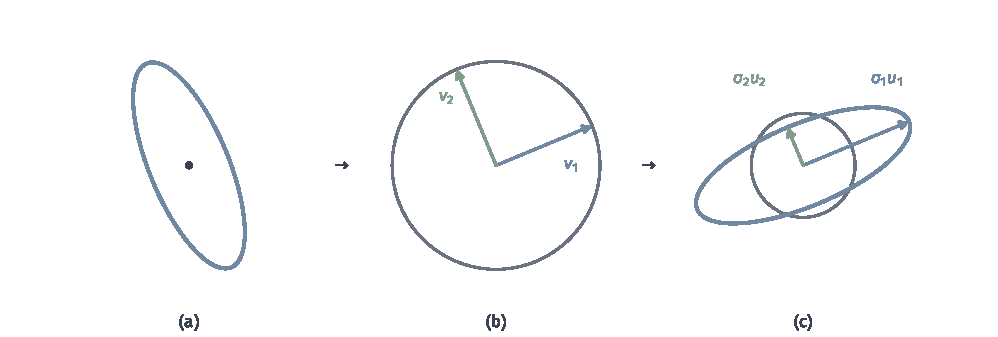
\includegraphics[width=168.998mm]{figures/00-shared/mathematical-preliminaries-upper/02-linear-spaces/matplotlib/ls-svd-construction/ls-svd-construction.pdf}
  \caption{SVD的三步构造。取$\bm A=\left[\begin{smallmatrix}2&0.5\\0.5&1\end{smallmatrix}\right]$，$\bm G=\bm A^\top\bm A=\left[\begin{smallmatrix}4.25&1.5\\1.5&1.25\end{smallmatrix}\right]$。(a)~二次型等值线$\bm x^\top\bm G\bm x=2$；(b)~$\bm G$的标准正交特征方向$\bm v_1,\bm v_2$，特征值约为$4.87,0.63$；(c)~单位圆及其在$\bm A$下的像，箭头为$\bm A\bm v_i=\sigma_i\bm u_i$，$\sigma_i=\sqrt{\lambda_i}\approx2.21,0.79$。各面板单独设定显示尺度。}
  \label{fig:ls-svd-construction}
\end{figure*}

左奇异向量与输出端也有对称的关系。对$i\leq r$，
\[
 \bm A^\top\bm u_i=\bm A^\top\bm A\bm v_i/\sigma_i=\sigma_i\bm v_i .
\]
对$i>r$，$\bm u_i$与$\operatorname{range}(\bm A)$正交，故对任意$\bm x$有
\[
 (\bm A^\top\bm u_i)^\top\bm x=\bm u_i^\top\bm A\bm x=0 ,
\]
即$\bm A^\top\bm u_i=\bm0$。于是
\begin{equation}
 \bm A^\top\bm u_i=\sigma_i\bm v_i,\qquad
 \bm A\bm A^\top\bm u_i=\sigma_i^2\bm u_i\qquad(i\leq r),
 \label{eq:ls-svd-transpose-relation}
\end{equation}
而$i>r$时$\bm A\bm A^\top\bm u_i=\bm0$。

也就是说，$\bm u_1,\ldots,\bm u_m$是$\bm A\bm A^\top$的一组标准正交特征向量，特征值依次为$\sigma_1^2,\ldots,\sigma_r^2$与$m-r$个零。$\bm A^\top\bm A$与$\bm A\bm A^\top$因而有相同的正特征值，分别在输入端与输出端给出奇异方向。

构造路线只用于证明存在性，并不意味着数值计算应当显式形成$\bm A^\top\bm A$；这一点在第~\ref{sec:svd-computation}节说明。

\subsection{奇异值分解的形式}
\label{sec:svd-forms}

定理~\ref{thm:ls-svd-existence}中的$\bm U$、$\bm V$都是方阵，这是\emph{完整}分解，它同时给出两端的全部正交方向：$\bm v_{r+1},\ldots,\bm v_d$张成$\ker\bm A$，$\bm u_{r+1},\ldots,\bm u_m$张成$\operatorname{range}(\bm A)$的正交补。三个因子的形状依次为$m\times m$、$m\times d$与$d\times d$。

许多计算只用到前$p=\min(m,d)$列。令$\bm U_p=[\bm u_1,\ldots,\bm u_p]\in\mathbb R^{m\times p}$、$\bm V_p=[\bm v_1,\ldots,\bm v_p]\in\mathbb R^{d\times p}$、$\bm\Sigma_p=\operatorname{diag}(\sigma_1,\ldots,\sigma_p)\in\mathbb R^{p\times p}$，则
\[
 \bm A=\bm U_p\bm\Sigma_p\bm V_p^\top ,
\]
称为\term{薄奇异值分解}（thin SVD），也称经济型分解。它由完整分解删去$\bm\Sigma$中全为零的那些行或列，连同与之相乘的$\bm U$或$\bm V$的列得到，乘积不变。$m\geq d$时删去的是$\bm U$的后$m-d$列，$m<d$时删去的是$\bm V$的后$d-m$列。

若只保留正奇异值，令$\bm U_r$、$\bm V_r$分别由前$r$个左、右奇异向量组成，$\bm\Sigma_r=\operatorname{diag}(\sigma_1,\ldots,\sigma_r)$，则
\[
 \begin{gathered}
 \bm A=\bm U_r\bm\Sigma_r\bm V_r^\top,\\
 \bm U_r\in\mathbb R^{m\times r},\quad\bm\Sigma_r\in\mathbb R^{r\times r},\quad\bm V_r\in\mathbb R^{d\times r},
 \end{gathered}
\]
这就是和式~\eqref{eq:matrix-analysis-svd-rank-one-sum}的矩阵写法，称为秩分解形式。

三种写法给出同一个矩阵，区别在于是否保留零伸缩的方向。秩分解只描述$\bm A$真正起作用的$r$对方向，$\bm U_r$与$\bm V_r$只是列标准正交，不再是方阵；零空间与输出端正交补的基要从完整分解中读取。薄分解在$r<p$时仍保留奇异值为零的列。三者都是$\bm A$的精确表示；只保留前$k<r$项、从而改变矩阵的截断近似，在第~\ref{chap:matrix-approximation}章讨论。

\subsection{奇异值分解的唯一性}
\label{sec:svd-uniqueness}

构造中有两处选择：$\bm A^\top\bm A$的标准正交特征基怎样选，以及输出端怎样补全。所以奇异值分解一般不唯一。本小节确定哪些部分由$\bm A$唯一决定。

先看奇异值。设$\bm A=\bm U\bm\Sigma\bm V^\top$是任意一个满足定理~\ref{thm:ls-svd-existence}的分解，则
\[
 \bm A^\top\bm A=\bm V(\bm\Sigma^\top\bm\Sigma)\bm V^\top ,
\]
其中$\bm\Sigma^\top\bm\Sigma$是$d$阶对角矩阵，对角元为$\sigma_1^2,\ldots,\sigma_{\min(m,d)}^2$，$d>m$时再补$d-m$个零。

$\bm V^\top=\bm V^{-1}$，所以$\bm A^\top\bm A$与$\bm\Sigma^\top\bm\Sigma$相似。由定理~\ref{thm:ls-spectrum-similarity-invariance}，二者有相同的特征多项式，$\sigma_i^2$连同重数恰是$\bm A^\top\bm A$的特征值。

$\bm A^\top\bm A$只依赖$\bm A$，而$\sigma_i$是这些特征值降序排列后的非负平方根，因此与分解的选取无关：正奇异值是$\bm A^\top\bm A$正特征值的平方根，其余为零。

奇异向量则可以变化。最简单的变化是把一对$\bm u_i,\bm v_i$同时变号：乘积$\sigma_i\bm u_i\bm v_i^\top$不变，两组向量仍各自标准正交。

奇异值重复时变化更多，例如$\bm A=\bm I_2$的奇异值都是$1$，对任意正交矩阵$\bm R$，$\bm I_2=\bm R\bm I_2\bm R^\top$都是奇异值分解。但两端不能各自独立地换：$\bm R_1\bm I_2\bm R_2^\top=\bm I_2$迫使$\bm R_1=\bm R_2$。下面的定理说明，这些例子已经包括了全部的自由度。

\begin{theorem}[奇异值分解的唯一性范围]
\label{thm:svd-uniqueness}
设$\bm A\in\mathbb R^{m\times d}$，$r=\operatorname{rank}\bm A$，$\bm A=\bm U\bm\Sigma\bm V^\top$是一个奇异值分解。对每个正奇异值$\sigma$，把$\bm V$、$\bm U$中满足$\sigma_i=\sigma$的列分别排成$\bm V_\sigma$、$\bm U_\sigma$；把$\bm V$的后$d-r$列与$\bm U$的后$m-r$列分别排成$\bm V_0$、$\bm U_0$。则：
\begin{enumerate}
 \item $\bm V_\sigma$与$\bm U_\sigma$的列空间分别是$\ker(\bm A^\top\bm A-\sigma^2\bm I)$与$\ker(\bm A\bm A^\top-\sigma^2\bm I)$，且$\bm U_\sigma=\bm A\bm V_\sigma/\sigma$；$\bm V_0$与$\bm U_0$的列空间分别是$\ker\bm A$与$\operatorname{range}(\bm A)^\perp$。
 \item 若$\bm A=\bm U'\bm\Sigma\bm V'^\top$是另一个奇异值分解，相应的分组记为$\bm V'_\sigma$等，则对每个正奇异值$\sigma$存在正交矩阵$\bm R_\sigma$，使
 \[
  \bm V'_\sigma=\bm V_\sigma\bm R_\sigma,\qquad\bm U'_\sigma=\bm U_\sigma\bm R_\sigma .
 \]
 \item 反过来，把$\bm V_0$、$\bm U_0$分别换成$\ker\bm A$与$\operatorname{range}(\bm A)^\perp$的任意标准正交基，或对某个$\sigma$同时右乘同一个正交矩阵$\bm R_\sigma$，所得仍是奇异值分解。
\end{enumerate}
特别地，每个正奇异值对应的项$\sigma\bm U_\sigma\bm V_\sigma^\top$由$\bm A$唯一确定。
\end{theorem}
\begin{proof}
(1)由$\bm A\bm V=\bm U\bm\Sigma$与$\bm A^\top\bm U=\bm V\bm\Sigma^\top$逐列读出
\[
 \bm A\bm v_i=\sigma_i\bm u_i,\qquad\bm A^\top\bm u_i=\sigma_i\bm v_i\qquad(i\leq\min(m,d)),
\]
其余列被$\bm A$或$\bm A^\top$送到零。于是
\[
 \bm A^\top\bm A\bm v_i=\sigma_i^2\bm v_i ,
\]
$\bm V$的各列是$\bm A^\top\bm A$的一组标准正交特征基，特征值依次为$\sigma_1^2,\ldots$，不足$d$个时补零。由谱投影定理~\ref{thm:ls-spectral-projections}的第一条，特征空间$\ker(\bm A^\top\bm A-\sigma^2\bm I)$恰由满足$\sigma_i^2=\sigma^2$的那些列张成，即$\bm V_\sigma$的列空间。

对$\bm A\bm A^\top=\bm U(\bm\Sigma\bm\Sigma^\top)\bm U^\top$同样讨论，得$\bm U_\sigma$的列空间。由$\bm A\bm v_i=\sigma\bm u_i$得$\bm U_\sigma=\bm A\bm V_\sigma/\sigma$。

$\bm V_0$的$d-r$列都满足$\bm A\bm v_i=\bm0$，彼此标准正交，而$\dim\ker\bm A=d-r$，所以它们是$\ker\bm A$的基。$\bm U_0$的$m-r$列与$\bm u_1,\ldots,\bm u_r$正交，后者张成$\operatorname{range}(\bm A)$，而$\dim\operatorname{range}(\bm A)^\perp=m-r$，所以它们是$\operatorname{range}(\bm A)^\perp$的基。

(2)由第一条，$\bm V_\sigma$与$\bm V'_\sigma$的列是同一个子空间的两组标准正交基。与谱投影定理第四条的证明相同，$\bm R_\sigma=\bm V_\sigma^\top\bm V'_\sigma$是正交矩阵，且$\bm V'_\sigma=\bm V_\sigma\bm R_\sigma$。再由第一条用于两个分解，
\[
 \bm U'_\sigma=\frac1\sigma\bm A\bm V'_\sigma=\frac1\sigma\bm A\bm V_\sigma\bm R_\sigma=\bm U_\sigma\bm R_\sigma .
\]

(3)分解按奇异值分组可以写成
\[
 \bm A=\sum_{\sigma>0}\sigma\bm U_\sigma\bm V_\sigma^\top ,
\]
其中不出现$\bm V_0$与$\bm U_0$，所以替换它们不改变乘积。新的列仍与其余列正交：$\ker\bm A$是$\operatorname{span}\{\bm v_1,\ldots,\bm v_r\}$的正交补，$\operatorname{range}(\bm A)^\perp$是$\operatorname{span}\{\bm u_1,\ldots,\bm u_r\}$的正交补，所以$\bm U$、$\bm V$仍是正交矩阵。

同时右乘$\bm R_\sigma$时，
\[
 \bm U_\sigma\bm R_\sigma(\bm V_\sigma\bm R_\sigma)^\top=\bm U_\sigma\bm V_\sigma^\top ,
\]
乘积不变，列仍标准正交。

最后一句由第二条得到：
\[
 \bm U'_\sigma\bm V_\sigma'^\top=\bm U_\sigma\bm R_\sigma\bm R_\sigma^\top\bm V_\sigma^\top=\bm U_\sigma\bm V_\sigma^\top .
\]
\end{proof}

于是，奇异值和每个正奇异值对应的左、右奇异子空间都由$\bm A$决定；同一个奇异值内部，左右两组基必须用同一个正交矩阵一起旋转，因为它们由$\bm u=\bm A\bm v/\sigma$配对。零奇异值的两部分则彼此独立，可以分别任意选取。若正奇异值互不相同，每个$\bm R_\sigma$都是$1\times1$的正交矩阵$\pm1$，奇异向量对只差一个公共的符号。这与第~\ref{sec:ls-spectral-projections}节的情形相仿：具体的向量可以变，子空间和合并后的项不变。

\subsection{奇异值分解的几何解释}
\label{sec:svd-geometry}


几何上，SVD把$\bm A$的作用拆成三步：$\bm V^\top$把输入写成右奇异方向上的坐标，$\bm\Sigma$把第$i$个坐标乘以$\sigma_i$，$\bm U$再把结果放到输出空间的左奇异方向上。正交矩阵保持长度，所以只有中间一步改变长度。于是$\bm A$把输入端的单位球映成输出空间中一个椭球；秩亏时这个椭球落在低维子空间内。

具体地，单位球中的$\bm x=\sum_ic_i\bm v_i$满足$\sum_ic_i^2\leq1$，其像为
\[
 \bm y=\sum_{i\leq r}\sigma_ic_i\bm u_i ,
\]
它落在$\operatorname{span}\{\bm u_1,\ldots,\bm u_r\}$中。坐标$y_i=\bm u_i^\top\bm y=\sigma_ic_i$满足
\[
 \sum_{i\leq r}(y_i/\sigma_i)^2=\sum_{i\leq r}c_i^2\leq1 .
\]

反过来，该子空间中满足这一不等式的$\bm y$是$\bm x=\sum_{i\leq r}(y_i/\sigma_i)\bm v_i$的像，而这个$\bm x$在单位球中。所以像恰为
\[
 \Bigl\{\bm y\in\operatorname{span}\{\bm u_1,\ldots,\bm u_r\}:\ \sum_{i=1}^r\frac{(\bm u_i^\top\bm y)^2}{\sigma_i^2}\leq1\Bigr\},
\]
即以$\sigma_i\bm u_i$为半轴的椭球：$\bm v_i$方向的单位向量被送到半轴端点$\sigma_i\bm u_i$。

若$r<d$，单位球面上的点也可能映到这个椭球的内部，例如$(\bm v_1+\bm v_d)/\sqrt2$被送到$\sigma_1\bm u_1/\sqrt2$，所以这里用单位球而不是球面描述整个像。

按这一图像，最长半轴就是最强的放大，第~\ref{sec:ls-svd-matrix-size}节将证明它等于$\lVert\bm A\rVert_2$，各半轴长度的平方和等于$\lVert\bm A\rVert_{\mathrm F}^2$。图~\ref{fig:matrix-analysis-svd-geometry}用二维旋转矩阵$\bm R(\theta)=\left[\begin{smallmatrix}\cos\theta&-\sin\theta\\\sin\theta&\cos\theta\end{smallmatrix}\right]$构造了一个输入方向与输出方向不同的例子。

\begin{figure*}[htbp]
  \centering
  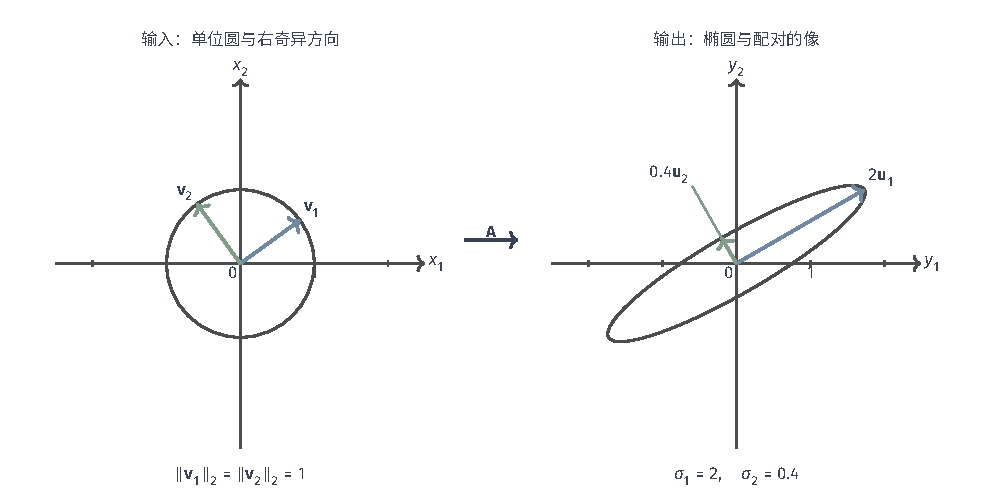
\includegraphics[width=168.998mm]{figures/00-shared/mathematical-preliminaries-upper/02-linear-spaces/tikz/matrix-analysis-svd-geometry/figure.pdf}
  \caption{矩阵$\bm A=\bm R(\pi/6)\operatorname{diag}(2,0.4)\bm R(\pi/5)^\top$
  将单位圆变为椭圆。蓝、绿分别对应两个奇异方向；同色箭头在左侧标出$\bm v_i$，
  在右侧标出其像$\sigma_i\bm u_i$。两侧坐标比例相同。奇异值决定长度变化，左右方向可以不同，
  因而这不是沿特征方向的同空间缩放。图为教学构造。}
  \label{fig:matrix-analysis-svd-geometry}
\end{figure*}

\subsection{奇异值分解的计算与核验}
\label{sec:svd-computation}
\phantomsection
\label{sec:svd-verification-geometry}

存在性定理的证明已经给出一条构造路线。对手算规模的矩阵$\bm A\in\mathbb R^{m\times d}$，可以按以下次序求出三个因子。先求对称半正定矩阵$\bm A^\top\bm A$的全部特征值，按降序记为$\lambda_1\geq\cdots\geq\lambda_d\geq0$，开方得到奇异值$\sigma_i=\sqrt{\lambda_i}$，正奇异值的个数就是$r=\operatorname{rank}\bm A$。再按第~\ref{sec:ls-spectral-decomposition-computation}节的方法求$\bm A^\top\bm A$的一组标准正交特征向量$\bm v_1,\ldots,\bm v_d$，排成$\bm V$，次序与特征值一致。然后对$i\leq r$令$\bm u_i=\bm A\bm v_i/\sigma_i$。最后若$r<m$，把$\bm u_1,\ldots,\bm u_r$补成$\mathbb R^m$的标准正交基，例如取$\ker\bm A^\top$的一组标准正交基作为$\bm u_{r+1},\ldots,\bm u_m$，排成$\bm U$。

第三步得到的向量自动标准正交，不必再正交化。对$i,j\leq r$，
\[
 \bm u_i^\top\bm u_j=\frac{\bm v_i^\top\bm A^\top\bm A\bm v_j}{\sigma_i\sigma_j}=\frac{\lambda_j\,\bm v_i^\top\bm v_j}{\sigma_i\sigma_j},
\]
$i\neq j$时为零，$i=j$时为$\lambda_i/\sigma_i^2=1$。补全的方向取在$\ker\bm A^\top=\operatorname{range}(\bm A)^\perp$中，与前$r$个方向自动垂直。

算出三个因子之后，或者拿到别人给出的一组因子时，要逐项核验。需要检查三件事：$\bm U^\top\bm U=\bm I$与$\bm V^\top\bm V=\bm I$；$\bm\Sigma$只有非负的对角元，并按降序排列；$\bm A\bm V=\bm U\bm\Sigma$，逐列看就是$\bm A\bm v_i=\sigma_i\bm u_i$。三项都成立时，在$\bm A\bm V=\bm U\bm\Sigma$两边右乘$\bm V^\top$，由$\bm V\bm V^\top=\bm I$即得$\bm A=\bm U\bm\Sigma\bm V^\top$。

正交性不能省略。若只核对乘积，任何分解$\bm A=\bm B\bm C$都可以写成$\bm U=\bm B$、$\bm\Sigma=\bm I$、$\bm V^\top=\bm C$的形式，却与奇异值毫无关系。另一方面，$\bm A^\top\bm U=\bm V\bm\Sigma^\top$由前三项推出，可以作为附加检查，它同时检验左奇异向量是否是$\bm A\bm A^\top$的特征向量。

\begin{example}[二阶矩阵的奇异值分解与核验]
\label{ex:svd-two-by-two-check}
下面用以下不对称的二阶矩阵演示：
\[
 \bm A=\begin{bmatrix}3&0\\4&5\end{bmatrix}.
\]
我们按上面的次序求出它的奇异值分解，再按三项逐一核验。

构造从对称矩阵$\bm A^\top\bm A$出发：
\[
 \bm A^\top\bm A=\begin{bmatrix}25&20\\20&25\end{bmatrix}.
\]
它的特征多项式为
\[
 (z-25)^2-400=(z-45)(z-5),
\]
特征值为$45$与$5$，对应的单位特征向量为$\bm v_1=(1,1)^\top/\sqrt2$与$\bm v_2=(1,-1)^\top/\sqrt2$。它们就是右奇异向量。特征值开方得到奇异值
\[
 \sigma_1=\sqrt{45}=3\sqrt5,\qquad\sigma_2=\sqrt5 .
\]

输出端的方向不必另解方程，由$\bm u_i=\bm A\bm v_i/\sigma_i$直接得到：
\[
 \begin{aligned}
 \bm u_1&=\frac{1}{3\sqrt5}\cdot\frac1{\sqrt2}\begin{bmatrix}3\\9\end{bmatrix}=\frac1{\sqrt{10}}\begin{bmatrix}1\\3\end{bmatrix},\\
 \bm u_2&=\frac{1}{\sqrt5}\cdot\frac1{\sqrt2}\begin{bmatrix}3\\-1\end{bmatrix}=\frac1{\sqrt{10}}\begin{bmatrix}3\\-1\end{bmatrix}.
 \end{aligned}
\]

接着逐项核验。正交性：
\[
 \bm u_1^\top\bm u_2=(3-3)/10=0 ,
\]
两者长度为$1$，$\bm v_1,\bm v_2$同样标准正交。对角元：$\sigma_1\geq\sigma_2>0$，非负且降序。

乘积：按秩一和式重建，
\[
 \begin{aligned}
 \sigma_1\bm u_1\bm v_1^\top+\sigma_2\bm u_2\bm v_2^\top
 &=\frac32\begin{bmatrix}1&1\\3&3\end{bmatrix}+\frac12\begin{bmatrix}3&-3\\-1&1\end{bmatrix}\\
 &=\begin{bmatrix}3&0\\4&5\end{bmatrix}=\bm A ,
 \end{aligned}
\]
其中$\sigma_1/\sqrt{20}=3/2$，$\sigma_2/\sqrt{20}=1/2$。

作为附加检查，
\[
 \bm A^\top\bm u_1=(15,15)^\top/\sqrt{10}=3\sqrt5\,\bm v_1 ,
\]
与式~\eqref{eq:ls-svd-transpose-relation}相符。

有了分解，第~\ref{sec:ls-svd-matrix-size}节将说明的几项大小就能直接读出：$\lVert\bm A\rVert_2=3\sqrt5\approx6.71$；$\lVert\bm A\rVert_{\mathrm F}^2=45+5=50$，与逐元素平方和$9+16+25$一致；两个奇异值都为正，$\bm A$可逆，且$\lVert\bm A^{-1}\rVert_2=1/\sqrt5$。
\end{example}

这个矩阵不对称，它的特征值是对角元$3$与$5$，与奇异值$6.71$、$2.24$都不同。特征值描述沿特征方向的倍数，奇异值描述把输入方向送到另一组正交方向时的倍数。对称半正定矩阵的奇异值就是它的特征值（第~\ref{sec:svd-orthogonal-coordinates}节），一般矩阵二者不同。

\paragraph{数值计算中的核验}

上面的构造与核验都是精确的代数运算。数值软件返回的因子$\widehat{\bm U}$、$\widehat{\bm\Sigma}$、$\widehat{\bm V}$带有舍入误差，各项等式只能近似成立，所以要分别报告两类残差。一类是重建误差
\[
 \lVert\bm A-\widehat{\bm U}\widehat{\bm\Sigma}\widehat{\bm V}^\top\rVert/\lVert\bm A\rVert ,
\]
另一类是正交性误差
\[
 \lVert\widehat{\bm U}^\top\widehat{\bm U}-\bm I\rVert,\qquad\lVert\widehat{\bm V}^\top\widehat{\bm V}-\bm I\rVert .
\]

两类残差不能互相代替。前面的例子已经说明，重建误差为零并不保证因子正交；反过来，两组列都正交、乘积却不等于$\bm A$，也只说明找到了某种正交矩阵。只有两类残差都小，才能把$\widehat{\bm\Sigma}$的对角元当作$\bm A$的奇异值的近似值；它们离真实奇异值有多远，由第~\ref{chap:condition-and-spectral-perturbation}章的奇异值扰动界判断。

构造路线从$\bm A^\top\bm A$出发，这条路线适合证明存在性，却不宜照搬到数值计算中。$\bm A^\top\bm A$的特征值是$\sigma_i^2$，最大与最小奇异值之比在其中变成平方，小奇异值相对于大奇异值变得更小，容易被舍入误差淹没。第~\ref{sec:ls-ls-regularization-sensitivity}节以最小二乘的正规方程为例分析这种平方带来的误差风险。实际计算奇异值分解的算法直接作用于$\bm A$本身，其构造与误差分析不在本书展开。

\section{奇异值与矩阵范数}
\label{sec:ls-svd-matrix-size}

第~\ref{sec:ls-frobenius-norm}节与第~\ref{sec:ls-matrix-norms}节分别定义了Frobenius范数与谱范数，但没有给出谱范数的算法。奇异值分解把这个问题化为比较坐标的平方和。

为了统一书写，把零伸缩也计入。对$\bm x\in\mathbb R^d$，写$\bm x=\sum_{i=1}^dc_i\bm v_i$，其中$c_i=\bm v_i^\top\bm x$，并约定$i>\min(m,d)$时$\sigma_i=0$。于是对每个$i\leq d$都有$\bm A\bm v_i=\sigma_i\bm u_i$或$\bm A\bm v_i=\bm0$，后者对应$\sigma_i=0$。由$\bm u_i$标准正交与$\bm v_i$标准正交，
\begin{equation}
 \lVert\bm A\bm x\rVert_2^2=\sum_{i=1}^d\sigma_i^2c_i^2,\qquad
 \lVert\bm x\rVert_2^2=\sum_{i=1}^dc_i^2 .
 \label{eq:svd-output-length}
\end{equation}

输出长度的平方是各$\sigma_i^2$以$c_i^2$为权的和。各$\sigma_i^2$都不超过最大的$\sigma_1^2$，也不小于补零后最小的$\sigma_d^2$，所以
\[
 \sigma_d\lVert\bm x\rVert_2\leq\lVert\bm A\bm x\rVert_2\leq\sigma_1\lVert\bm x\rVert_2 ,
\]
这里$d>m$或$\operatorname{rank}\bm A<d$时$\sigma_d=0$。取$\bm x=\bm v_1$时只有$c_1=1$，上界取等号；取$\bm x=\bm v_d$时下界取等号。这一比较只用到坐标平方和，不涉及任何极值原理。

由上界及其可达性，单位输入的最大输出长度就是$\sigma_1$。

Frobenius范数则由迹的循环性得到：
\[
 \begin{aligned}
 \lVert\bm A\rVert_{\mathrm F}^2&=\operatorname{tr}(\bm A^\top\bm A)=\operatorname{tr}\bigl(\bm V(\bm\Sigma^\top\bm\Sigma)\bm V^\top\bigr)\\
 &=\operatorname{tr}(\bm\Sigma^\top\bm\Sigma\bm V^\top\bm V)=\sum_i\sigma_i^2 .
 \end{aligned}
\]
因此
\begin{align}
 \lVert\bm A\rVert_2&=\sigma_1,
 \label{eq:matrix-analysis-spectral-norm}\\
 \lVert\bm A\rVert_{\mathrm F}&=\Bigl(\sum_{i=1}^r\sigma_i^2\Bigr)^{1/2}.
 \label{eq:matrix-analysis-frobenius-norm}
\end{align}
正奇异值的个数等于$\operatorname{rank}\bm A$，这已在构造中证明。谱范数只看最强的一个伸缩，Frobenius范数把全部伸缩的平方加在一起，所以
\[
 \lVert\bm A\rVert_2\leq\lVert\bm A\rVert_{\mathrm F}\leq\sqrt r\,\lVert\bm A\rVert_2 .
\]

下界在秩亏时为零，并不提供信息。$\ker\bm A$中的非零输入被送到零，它们的输出长度不说明$\bm A$在其他方向上作用多弱。有意义的问题是在$\ker\bm A$的正交补$\operatorname{span}\{\bm v_1,\ldots,\bm v_r\}$上，单位输入至少被送出多远。满列秩时$\ker\bm A=\{\bm0\}$，这个正交补就是整个输入空间。可逆方阵的逆矩阵则把每个伸缩倍数倒过来，最弱的放大变成逆矩阵最强的放大。下面的定理汇总这几项读数。

\begin{theorem}[最小奇异值与逆矩阵的范数]
\label{thm:ls-svd-singular-value-norms}
设$\bm A\in\mathbb R^{m\times d}$的秩为$r\geq1$，奇异值分解如定理~\ref{thm:ls-svd-existence}所示。
\begin{enumerate}
 \item 对$\ker\bm A$的正交补中的任意$\bm x$，$\lVert\bm A\bm x\rVert_2\geq\sigma_r\lVert\bm x\rVert_2$，等号在$\bm x=\bm v_r$时成立。
 \item 若$\bm A$满列秩，即$r=d\leq m$，则对所有$\bm x\in\mathbb R^d$，$\lVert\bm A\bm x\rVert_2\geq\sigma_d\lVert\bm x\rVert_2$，且
 \[
  \min_{\lVert\bm x\rVert_2=1}\lVert\bm A\bm x\rVert_2=\sigma_d>0 .
 \]
 \item 若$\bm A$是可逆方阵（$m=d=r$），则$\bm A^{-1}=\sum_{i=1}^d\sigma_i^{-1}\bm v_i\bm u_i^\top$，并且
 \begin{equation}
  \lVert\bm A^{-1}\rVert_2=\frac1{\sigma_d}.
  \label{eq:ls-svd-inverse-norm}
 \end{equation}
\end{enumerate}
\end{theorem}
\begin{proof}
由构造，$\ker\bm A$由$\bm v_{r+1},\ldots,\bm v_d$张成，其正交补由$\bm v_1,\ldots,\bm v_r$张成。对其中的$\bm x=\sum_{i\leq r}c_i\bm v_i$，由式~\eqref{eq:svd-output-length}，
\[
 \lVert\bm A\bm x\rVert_2^2=\sum_{i\leq r}\sigma_i^2c_i^2\geq\sigma_r^2\sum_{i\leq r}c_i^2=\sigma_r^2\lVert\bm x\rVert_2^2 ,
\]
其中用到$\sigma_i\geq\sigma_r$（$i\leq r$）；取$\bm x=\bm v_r$时只有$c_r=1$，等号成立。这是第一条。

满列秩时正交补就是$\mathbb R^d$，且$\sigma_r=\sigma_d>0$，第一条即给出第二条。

对第三条，令$\bm B=\sum_i\sigma_i^{-1}\bm v_i\bm u_i^\top$。由$\bm v_i^\top\bm v_j=\delta_{i,j}$，
\[
 \begin{aligned}
 \bm A\bm B&=\sum_{i,j}\sigma_i\sigma_j^{-1}\bm u_i(\bm v_i^\top\bm v_j)\bm u_j^\top\\
 &=\sum_i\bm u_i\bm u_i^\top=\bm U\bm U^\top=\bm I,
 \end{aligned}
\]
方阵的右逆就是逆，所以$\bm B=\bm A^{-1}$。

这个和式本身就是$\bm A^{-1}$的奇异值分解：右奇异向量为$\bm u_i$，左奇异向量为$\bm v_i$，奇异值为$\sigma_i^{-1}$，其中最大的是$\sigma_d^{-1}$。由式~\eqref{eq:matrix-analysis-spectral-norm}，$\lVert\bm A^{-1}\rVert_2=1/\sigma_d$。
\end{proof}

满列秩只保证最小放大倍数为正，并不保证它不太小。式~\eqref{eq:ls-svd-inverse-norm}说明，最小奇异值越小，逆矩阵把输出端的误差放大得越厉害。最大奇异值衡量最强的放大，最小奇异值衡量最弱的放大，二者之比就是第~\ref{sec:ls-matrix-condition-number}节的矩阵条件数，它决定线性方程的解对数据误差有多敏感。

当$r<d$时（$m<d$时总是如此），存在非零输入被送到零，单位输入的最小输出长度为零，这时只能在零空间的正交补上谈最弱的放大。最弱放大的方向$\bm v_d$也有直接用处：第~\ref{sec:linear-algebra-homogeneous-estimation}节的齐次最小二乘在单位向量中最小化$\lVert\bm A\bm x\rVert_2$，由上面的下界及其取等条件，最优解就是$\bm v_d$。

本节的上下界是对单个输入的比较。若要在所有$k$维子空间中挑出保留输出能量最多的一个，就需要比较子空间，这是第~\ref{chap:matrix-approximation}章用Rayleigh商和迹极值处理的最优选择问题。

\FloatBarrier
\section{本章小结}
\label{sec:svd-chapter-summary}

本章开头问：输入、输出各取一组标准正交基时，是否任何矩阵都能化为对角形？答案是肯定的。由$\bm A^\top\bm A$的谱分解取右奇异向量$\bm v_i$，开方得到奇异值$\sigma_i$，再令$\bm u_i=\bm A\bm v_i/\sigma_i$并补全，就得到$\bm A=\bm U\bm\Sigma\bm V^\top$，即$\bm A\bm v_i=\sigma_i\bm u_i$。这一构造只依赖谱定理，对矩形矩阵、不能对角化的方阵和非正规方阵都成立。

分解有完整、薄与秩分解三种写法，区别只在是否保留零伸缩的方向。奇异值由$\bm A$唯一确定，是$\bm A^\top\bm A$特征值的非负平方根；每个正奇异值的左、右奇异子空间也唯一，同一奇异值内部的两组基只能用同一个正交矩阵一起旋转。零奇异值对应的$\ker\bm A$与$\operatorname{range}(\bm A)^\perp$的基则可以各自任意选取。

在奇异坐标中，输出长度的平方是$\sum_i\sigma_i^2c_i^2$。由此直接读出$\lVert\bm A\rVert_2=\sigma_1$、$\lVert\bm A\rVert_{\mathrm F}^2=\sum_i\sigma_i^2$、$\operatorname{rank}\bm A$等于正奇异值的个数；在零空间的正交补上最弱的放大是$\sigma_r$，可逆方阵的$\lVert\bm A^{-1}\rVert_2=1/\sigma_d$。几何上，$\bm A$把单位球映成以$\sigma_i\bm u_i$为半轴的椭球。

核验一组因子要同时检查正交性与$\bm A\bm V=\bm U\bm\Sigma$；数值计算中重建误差和正交性误差须分别报告，并且不宜通过显式形成$\bm A^\top\bm A$来计算。

这些读数将在后面几章使用。第~\ref{chap:polar-decomposition}章由奇异值分解把矩阵分成伸缩与保长两部分，第~\ref{chap:condition-and-spectral-perturbation}章用$\sigma_{\max}/\sigma_{\min}$度量误差放大，并估计奇异值本身受扰动时的变化。按奇异值从大到小保留方向、得到最佳低秩近似，是第~\ref{chap:matrix-approximation}章的任务。

% 第8章：极分解（伸缩与正交转向的分离、可逆方阵、奇异方阵与矩形矩阵的极分解、矩阵函数的谱表示）。

\chapter{极分解}
\label{sec:ls-polar-decomposition}
\label{chap:polar-decomposition}

非零复数$z$可以写成$z=e^{\mathrm i\theta}r$：先乘正数$r$改变长度，再乘单位复数$e^{\mathrm i\theta}$转动方向。本章对矩阵提出同样的问题：给定$\bm A$，能否把它写成$\bm A=\bm W\bm H$，使$\bm H$沿一组互相垂直的方向作非负伸缩，$\bm W$保持长度？这样的分解是否唯一？先转向、后伸缩是否也可以？矩阵奇异或不是方阵时，又能保留多少？

第~\ref{chap:singular-value-decomposition}章的奇异值分解已经把$\bm A$写成“转向、伸缩、再转向”的三段。本章把三段重新组合成两段，并关心另一个问题：两个因子能否直接由$\bm A$求出，而不先求出全部奇异向量。

第~\ref{sec:ls-polar-square-root-equation}节先讨论伸缩与正交转向怎样分离：利用正交因子保持长度把它消去，得到只含伸缩因子的开方方程，沿谱开方构造唯一的半正定伸缩因子，并据此定义极分解。伸缩因子在任何情形下都这样求出，正交因子的求法则随矩阵的情形而变，后面三节各处理一种情形：第~\ref{sec:ls-polar-orthogonal-factor}节处理可逆方阵，撤销伸缩即得唯一的正交因子，并比较先伸缩后转向与先转向后伸缩两种写法；第~\ref{sec:ls-polar-singular-best-orthogonal}节处理奇异方阵，借助奇异值分解构造正交因子，并说明核怎样使它失去唯一性；第~\ref{sec:ls-polar-rectangular}节处理矩形矩阵，说明保长因子只能是列标准正交或行标准正交的矩阵。

第~\ref{sec:ls-matrix-functions}节把开方和求逆中共同使用的“沿谱改写特征值”归纳为对称矩阵的函数。

本章用到第~\ref{chap:eigen-spectral-decomposition}章的谱定理、谱投影与定号性判据，奇异情形还用到第~\ref{chap:singular-value-decomposition}章的奇异值分解。极分解的正交因子还有一个最优性：第~\ref{chap:matrix-approximation}章将证明，在Frobenius范数下它是离$\bm A$最近的正交矩阵（定理~\ref{thm:ls-best-orthogonal-approximation}）。这需要比较全部正交矩阵，属于约束下的矩阵逼近问题，本章不展开。

\section{伸缩与正交转向的分离}
\label{sec:ls-polar-square-root-equation}

本节说明伸缩与转向怎样分开：先消去正交因子，得到只含伸缩因子的开方方程；再沿谱开方，构造唯一的半正定伸缩因子；最后据此定义极分解，并说明正交因子的求法为什么要按情形讨论。

\subsection{开方方程}
\label{sec:ls-polar-square-root-subsection}

先看一个具体矩阵。本章用以下矩阵作为贯穿例：
\[
 \bm A=\begin{bmatrix}0&-1\\3&0\end{bmatrix}.
\]
它把$\bm e_1$送到$3\bm e_2$，把$\bm e_2$送到$-\bm e_1$。这个作用既改变长度，又改变方向：$\bm e_1$被拉长为原来的$3$倍，同时两个坐标轴都被转了$90$度。我们希望把它拆成两步：先由对称正定的$\bm H$沿一组正交方向伸缩，再由正交矩阵$\bm W$保长地改变方向，即求$\bm A=\bm W\bm H$。

本节的推导对一般方阵$\bm A\in\mathbb R^{d\times d}$成立，例子取可逆矩阵。$\bm A$可逆时，它不把任何非零向量压成零，伸缩可以撤销，所求的$\bm H$应当正定；$\bm A$奇异时，有些方向被压成零，$\bm H$只能半正定。正交矩阵既可以是旋转，也可以包含反射，这里不加限制。矩形矩阵的情形在第~\ref{sec:ls-polar-rectangular}节处理。

两个因子同时未知，先设法消去一个。若$\bm A=\bm W\bm H$，其中$\bm W^\top\bm W=\bm I$、$\bm H^\top=\bm H$，则把等式两边分别转置后与原式相乘，得到
\begin{equation}
 \bm A^\top\bm A
 =\bm H^\top\bm W^\top\bm W\bm H
 =\bm H^2 .
 \label{eq:ls-polar-square-root-equation}
\end{equation}
正交因子在相乘时消失了，因为它保持长度：
\[
 \lVert\bm A\bm x\rVert_2=\lVert\bm W\bm H\bm x\rVert_2=\lVert\bm H\bm x\rVert_2 .
\]

记$\bm S=\bm A^\top\bm A$，它完全由已知的$\bm A$确定。于是原问题的前一半化为一个开方问题：找一个对称正定矩阵$\bm H$，使$\bm H^2=\bm S$。需要注意，式~\eqref{eq:ls-polar-square-root-equation}只是分解若存在就必须满足的条件；这样的$\bm H$是否存在、由它能否再得到正交的$\bm W$，都还没有证明。

开方之前先确认$\bm S$的结构。它对称，因为$(\bm A^\top\bm A)^\top=\bm A^\top\bm A$；对任意$\bm x$，
\[
 \bm x^\top\bm S\bm x=(\bm A\bm x)^\top(\bm A\bm x)=\lVert\bm A\bm x\rVert_2^2\geq0,
\]
所以$\bm S$对称半正定，可以使用第~\ref{sec:ls-spectral-theory}节的正交谱分解，全部特征值非负。$\bm A$可逆时，非零$\bm x$使$\bm A\bm x\neq\bm0$，上式严格大于零，$\bm S$正定，全部特征值为正。

在贯穿例中，先算出$\bm S$：
\[
 \begin{aligned}
 \bm S=\bm A^\top\bm A
 &=\begin{bmatrix}0&3\\-1&0\end{bmatrix}
 \begin{bmatrix}0&-1\\3&0\end{bmatrix}\\
 &=\begin{bmatrix}9&0\\0&1\end{bmatrix}.
 \end{aligned}
\]
这里$\bm S$恰好是对角矩阵，最直接的做法是沿两个坐标轴分别取正平方根，得到候选$\bm H=\operatorname{diag}(3,1)$。一般的$\bm S$不是对角矩阵，下一小节用谱分解把它化到这种情形。

\subsection{伸缩因子的构造}
\label{sec:ls-matrix-square-root}

对上一小节的$\bm S=\bm A^\top\bm A$作正交谱分解
\[
 \bm S=\bm Q\bm\Lambda\bm Q^\top,
\]
其中$\bm Q=[\bm q_1,\ldots,\bm q_d]$正交，$\bm\Lambda=\operatorname{diag}(\lambda_1,\ldots,\lambda_d)$，全部$\lambda_i\geq0$。先看$\bm A$可逆、全部$\lambda_i>0$的情形。

在特征方向$\bm q_i$上，$\bm S$只作标量伸缩$\lambda_i$倍。既然希望$\bm H$作用两次等于$\bm S$，自然尝试让$\bm H$沿同一方向伸缩$\sqrt{\lambda_i}$倍，即构造
\begin{equation}
 \bm H=\bm Q\operatorname{diag}\bigl(\sqrt{\lambda_1},\ldots,\sqrt{\lambda_d}\bigr)\bm Q^\top .
 \label{eq:ls-spectral-square-root}
\end{equation}
这是我们主动选取的一个候选，并没有预先假定未知的$\bm H$必须与$\bm S$共用特征基；它是否满足要求，要靠验证。

验证只需矩阵乘法。记$\bm\Lambda^{1/2}=\operatorname{diag}(\sqrt{\lambda_1},\ldots,\sqrt{\lambda_d})$，由$\bm Q^\top\bm Q=\bm I$，
\[
 \bm H^2
 =\bm Q\bm\Lambda^{1/2}(\bm Q^\top\bm Q)\bm\Lambda^{1/2}\bm Q^\top
 =\bm Q\bm\Lambda\bm Q^\top
 =\bm S .
\]
又
\[
 \bm H^\top=\bm Q(\bm\Lambda^{1/2})^\top\bm Q^\top=\bm H ,
\]
而式~\eqref{eq:ls-spectral-square-root}本身就是$\bm H$的正交谱分解，特征值$\sqrt{\lambda_i}$全为正，所以$\bm H$对称正定。

所需的伸缩因子已经求出，记作$\bm S^{1/2}$，称为$\bm S$的正定平方根，也称\term{矩阵平方根}（matrix square root）。

构造本身只用到$\lambda_i\geq0$，所以对半正定的$\bm S$同样可行，此时得到半正定的$\bm H$。还剩一个问题：$\bm Q$不唯一，特征值有重根时，重根空间内可以换用别的标准正交基。

方程$\bm X^2=\bm S$本身也可能有许多解。例如$\bm I$、$-\bm I$与$\operatorname{diag}(1,-1)$的平方都是$\bm I_2$，后两个对称却不半正定；不对称的$\left[\begin{smallmatrix}0&1\\0&0\end{smallmatrix}\right]$与零矩阵的平方都是零矩阵。

所以“平方等于$\bm S$”这一代数条件不足以确定伸缩因子。下面的定理说明，只要要求解对称半正定，答案就唯一，因而与$\bm Q$的选取无关。

\begin{theorem}[半正定平方根的存在与唯一]
\label{thm:ls-psd-square-root}
设$\bm S\in\mathbb R^{d\times d}$对称半正定，有正交谱分解$\bm S=\bm Q\bm\Lambda\bm Q^\top$。则存在唯一的对称半正定矩阵$\bm X$满足$\bm X^2=\bm S$，它就是式~\eqref{eq:ls-spectral-square-root}给出的$\bm S^{1/2}$。$\bm S$正定时，$\bm S^{1/2}$也正定。
\end{theorem}
\begin{proof}
存在性与正定性已由上面的验证给出：$\bm S$半正定时全部$\lambda_i\geq0$，$\sqrt{\lambda_i}$有定义，式~\eqref{eq:ls-spectral-square-root}是对称半正定矩阵且平方为$\bm S$；$\bm S$正定时全部$\sqrt{\lambda_i}>0$。

下证唯一性。设$\bm X$对称半正定且$\bm X^2=\bm S$。对$\bm X$本身作正交谱分解
\[
 \bm X=\sum_{j=1}^d\mu_j\bm p_j\bm p_j^\top ,
\]
其中$\bm p_1,\ldots,\bm p_d$是标准正交基，$\mu_j\geq0$。由$\bm p_j^\top\bm p_k=\delta_{j,k}$，
\[
 \bm S=\bm X^2=\sum_{j=1}^d\mu_j^2\bm p_j\bm p_j^\top ,
\]
所以$\bm S\bm p_j=\mu_j^2\bm p_j$，每个$\bm p_j$都是$\bm S$的特征向量。

取$\bm S$的任一特征值$\lambda$，考察特征空间$\ker(\bm S-\lambda\bm I)$。把任意$\bm x$展开为$\bm x=\sum_jc_j\bm p_j$，则
\[
 (\bm S-\lambda\bm I)\bm x=\sum_{j=1}^dc_j(\mu_j^2-\lambda)\bm p_j ,
\]
由$\bm p_j$线性无关，它为零当且仅当凡$\mu_j^2\neq\lambda$的$j$都有$c_j=0$。因此$\ker(\bm S-\lambda\bm I)$恰由满足$\mu_j^2=\lambda$的那些$\bm p_j$张成。

对这些$j$，$\mu_j\geq0$迫使$\mu_j=\sqrt\lambda$，于是对特征空间中的每个$\bm x$，
\[
 \bm X\bm x=\sum_{\mu_j^2=\lambda}c_j\mu_j\bm p_j=\sqrt\lambda\,\bm x .
\]
另一方面，由式~\eqref{eq:ls-spectral-square-root}，
\[
 \bm S^{1/2}\bm q_i=\sqrt{\lambda_i}\bm q_i ,
\]
而$\ker(\bm S-\lambda\bm I)$由满足$\lambda_i=\lambda$的$\bm q_i$张成，所以$\bm S^{1/2}$在这个特征空间上同样是乘以$\sqrt\lambda$。

这样，$\bm X$与$\bm S^{1/2}$在$\bm S$的每个特征空间上作用相同。由谱定理，这些特征空间合起来张成$\mathbb R^d$（各$\bm q_i$都落在其中某一个里），线性映射在一组基上相同即处处相同，故$\bm X=\bm S^{1/2}$。
\end{proof}

唯一性的论证直接说明了两件事。第一，在重根空间内换基，相应的$\bm q_i$变了，但特征空间和其上的作用“乘以$\sqrt\lambda$”不变，所以$\bm S^{1/2}$不依赖$\bm Q$的选取。第二，唯一性只针对半正定解；去掉这一要求，$\bm X^2=\bm S$一般有许多解，$-\bm S^{1/2}$就是其中之一。

在贯穿例中，$\bm S=\operatorname{diag}(9,1)$，可取$\bm Q=\bm I$，得到$\bm H=\operatorname{diag}(3,1)$。直接核对：
\[
 \bm H^2=\operatorname{diag}(9,1)=\bm S .
\]
上一小节凭直觉写出的候选正是唯一的正定平方根。

伸缩因子已经求出，正交因子的求法随矩阵的情形而变，放到后面三节讨论。

这里所做的“把每个特征值换成它的平方根”，将在第~\ref{sec:ls-matrix-functions}节成为矩阵函数的一个具体例子；但构造和验证本身只用到谱分解、标量开方与矩阵乘法。

所得的平方根带来一个后文直接使用的长度恒等式。由$\bm S^{1/2}$对称及$(\bm S^{1/2})^2=\bm S$，对半正定$\bm S$与任意$\bm x$，
\begin{equation}
 \lVert\bm S^{1/2}\bm x\rVert_2^2
 =\bm x^\top\bm S^{1/2}\bm S^{1/2}\bm x
 =\bm x^\top\bm S\bm x .
 \label{eq:ls-square-root-length}
\end{equation}
它把第~\ref{sec:ls-weighted-inner-products}节以$\bm S$加权的长度化为普通欧氏长度。

对$\bm S=\bm A^\top\bm A$，它给出
\[
 \lVert\bm H\bm x\rVert_2=\lVert\bm A\bm x\rVert_2 ,
\]
说明$\bm H$承担了$\bm A$的全部长度变化；但这并不表示$\bm H\bm x$与$\bm A\bm x$方向相同，方向的差别正要由$\bm W$补上。

第~\ref{chap:stationary-iterations}章分析Gauss--Seidel迭代的收缩时，就用式~\eqref{eq:ls-square-root-length}把能量范数写成欧氏长度。

\subsection{极分解的定义}
\label{sec:ls-polar-definition}

上两小节说明，若$\bm A$能写成正交因子与半正定伸缩因子之积，伸缩因子只能是$(\bm A^\top\bm A)^{1/2}$。把这样的分解单独命名。
\begin{definition}[极分解]
\label{def:matrix-analysis-polar-decomposition}
设$\bm A\in\mathbb R^{d\times d}$。若$\bm W$是正交矩阵，$\bm H$是对称半正定矩阵，且
\begin{equation}
\begin{gathered}
 \bm A=\bm W\bm H\\
 \bm W^\top\bm W=\bm I,\quad \bm H=(\bm A^\top\bm A)^{1/2},
\end{gathered}
\label{eq:matrix-analysis-polar-decomposition}
\end{equation}
则称$\bm A=\bm W\bm H$为$\bm A$的\term{极分解}（polar decomposition），也称右极分解，$\bm W$称为正交因子，$\bm H$称为伸缩因子。
\end{definition}

式中$\bm H=(\bm A^\top\bm A)^{1/2}$并不是额外的要求：由式~\eqref{eq:ls-polar-square-root-equation}，任何满足$\bm A=\bm W\bm H$、$\bm W$正交、$\bm H$对称半正定的分解都有$\bm H^2=\bm A^\top\bm A$，再由定理~\ref{thm:ls-psd-square-root}，$\bm H$只能是$(\bm A^\top\bm A)^{1/2}$。所以极分解中的伸缩因子总是唯一的，问题只在正交因子。

同一个作用也可以先转向、后伸缩，即求$\bm A=\bm K\bm W'$，其中$\bm K$对称半正定、$\bm W'$正交。仿照式~\eqref{eq:ls-polar-square-root-equation}，这次从右侧消去正交因子：
\[
 \bm A\bm A^\top=\bm K\bm W'\bm W'^\top\bm K^\top=\bm K^2 .
\]
所以$\bm K$只能是$\bm A\bm A^\top$的半正定平方根，$\bm A$可逆时它正定。这样的分解称为左极分解。$\bm A\bm A^\top$与$\bm A^\top\bm A$一般不同，左右两个伸缩因子也就不同。

剩下的是正交因子怎样求。它取决于$\bm A$是否可逆、是否为方阵：可逆方阵的伸缩因子可逆，撤销伸缩即得正交因子（第~\ref{sec:ls-polar-orthogonal-factor}节）；奇异方阵有被压成零的方向，正交因子要借助奇异值分解构造，并且不唯一（第~\ref{sec:ls-polar-singular-best-orthogonal}节）；矩形矩阵的输入与输出不在同一空间，保长因子只能是列标准正交或行标准正交的矩阵（第~\ref{sec:ls-polar-rectangular}节）。

\section{可逆矩阵的极分解}
\label{sec:ls-polar-orthogonal-factor}

可逆方阵的伸缩因子正定，因而可逆，正交因子可以直接由撤销伸缩求出。整个构造分四步：先算$\bm S=\bm A^\top\bm A$；再作正交谱分解$\bm S=\bm Q\bm\Lambda\bm Q^\top$，取$\bm H=\bm Q\bm\Lambda^{1/2}\bm Q^\top$；然后取$\bm H^{-1}=\bm Q\bm\Lambda^{-1/2}\bm Q^\top$，令$\bm W=\bm A\bm H^{-1}$；最后核验$\bm W^\top\bm W=\bm I$与$\bm W\bm H=\bm A$。本节依次说明这几步、证明两个因子唯一，再给出先转向后伸缩的左极分解。

\subsection{构造过程}
\label{sec:ls-polar-invertible-construction}

回到$\bm A=\bm W\bm H$。刚求出的$\bm H$正定，因而可逆，在等式两边右乘$\bm H^{-1}$，得到正交因子唯一可能的候选
\[
 \bm W=\bm A\bm H^{-1}.
\]
右乘而不是左乘，是由原方程中因子的顺序决定的：$\bm H$先作用，要撤销它的伸缩，就要在$\bm A$的右侧作用$\bm H^{-1}$。

$\bm H^{-1}$同样可以沿特征方向写出。$\bm H$沿$\bm q_i$伸缩$\sqrt{\lambda_i}$倍，撤销这一伸缩就是沿同一方向乘以$1/\sqrt{\lambda_i}$。令
\[
 \bm H^{-1}=\bm Q\operatorname{diag}\bigl(1/\sqrt{\lambda_1},\ldots,1/\sqrt{\lambda_d}\bigr)\bm Q^\top ,
\]
由$\bm Q^\top\bm Q=\bm I$，它与$\bm H$相乘得
\[
 \bm H\bm H^{-1}=\bm Q\bm\Lambda^{1/2}\bm\Lambda^{-1/2}\bm Q^\top=\bm Q\bm I\bm Q^\top=\bm I ,
\]
确实是逆矩阵。它也对称正定，记作$\bm S^{-1/2}$，称为$\bm S$的逆平方根。

定义了$\bm W=\bm A\bm H^{-1}$之后，必须检查它满足原来要求的性质。由$(\bm H^{-1})^\top=(\bm H^\top)^{-1}=\bm H^{-1}$及$\bm A^\top\bm A=\bm S=\bm H^2$，
\[
 \bm W^\top\bm W
 =\bm H^{-1}\bm A^\top\bm A\bm H^{-1}
 =\bm H^{-1}\bm H^2\bm H^{-1}
 =\bm I ,
\]
所以$\bm W$正交。又
\[
 \bm W\bm H=\bm A\bm H^{-1}\bm H=\bm A .
\]
正交性和分解等式都成立，存在性才算证完。

现在把贯穿例算完。$\bm H=\operatorname{diag}(3,1)$，所以$\bm H^{-1}=\operatorname{diag}(1/3,1)$，右乘得
\[
 \begin{aligned}
 \bm W=\bm A\bm H^{-1}
 &=\begin{bmatrix}0&-1\\3&0\end{bmatrix}
 \begin{bmatrix}1/3&0\\0&1\end{bmatrix}\\
 &=\begin{bmatrix}0&-1\\1&0\end{bmatrix}.
 \end{aligned}
\]
逐项核对：
\[
 \bm W^\top\bm W=\bm I,\qquad
 \bm W\bm H=\begin{bmatrix}0&-1\\3&0\end{bmatrix}=\bm A .
\]
$\bm W$把$\bm e_1$送到$\bm e_2$、把$\bm e_2$送到$-\bm e_1$，是逆时针旋转$90$度。

于是原变换可以读成：先沿$\bm e_1$伸长$3$倍、沿$\bm e_2$保持不变，再整体旋转$90$度。在这个解题过程中，$\bm S$是由$\bm A$直接算出的中间量，$\bm H$是对$\bm S$开方得到的因子，$\bm W$则是撤销伸缩后剩下的因子。

\subsection{唯一性}
\label{sec:ls-polar-invertible-uniqueness}

上面的构造给出了一组因子。下面的定理说明，可逆时极分解只有这一组。
\begin{theorem}[可逆矩阵的极分解]
\label{thm:ls-polar-invertible}
设$\bm A\in\mathbb R^{d\times d}$可逆，则$\bm A$有极分解，且两个因子都唯一：
\begin{equation}
 \bm H=(\bm A^\top\bm A)^{1/2},\qquad
 \bm W=\bm A(\bm A^\top\bm A)^{-1/2},
 \label{eq:ls-polar-invertible-factors}
\end{equation}
其中$\bm H$对称正定。
\end{theorem}
\begin{proof}
存在性：由第~\ref{sec:ls-polar-square-root-equation}节，$\bm S=\bm A^\top\bm A$对称正定；由定理~\ref{thm:ls-psd-square-root}，$\bm H=\bm S^{1/2}$对称正定，从而可逆；上面已验证$\bm W=\bm A\bm H^{-1}$正交且$\bm W\bm H=\bm A$。

唯一性：设$\bm A=\bm W'\bm H'$是任一极分解。由式~\eqref{eq:ls-polar-square-root-equation}，$\bm H'^2=\bm S$，又$\bm H'$对称半正定，由定理~\ref{thm:ls-psd-square-root}得$\bm H'=\bm S^{1/2}=\bm H$。

$\bm H$可逆，在$\bm A=\bm W'\bm H$两边右乘$\bm H^{-1}$得$\bm W'=\bm A\bm H^{-1}=\bm W$。
\end{proof}

由$\det\bm A=\det\bm W\det\bm H$及$\det\bm H>0$，$\det\bm W$与$\det\bm A$同号：$\det\bm A>0$时$\bm W$是旋转，$\det\bm A<0$时$\bm W$包含一次反射。这正是第~\ref{sec:ls-polar-square-root-equation}节不限制正交作用类型的原因。

第~\ref{sec:ls-matrix-square-root}节的长度恒等式还可以与Gram因子比较。若只需表示同一个长度，平方根并不是唯一的选择：由定理~\ref{thm:ls-gram-factor}，正定$\bm S$还可写成$\bm S=\bm L^\top\bm L$，$\bm L$可逆，此时同样有
\[
 \lVert\bm L\bm x\rVert_2^2=\bm x^\top\bm S\bm x=\lVert\bm S^{1/2}\bm x\rVert_2^2 .
\]
这只说明两个向量$\bm L\bm x$与$\bm S^{1/2}\bm x$长度相同，并不表示两个矩阵对向量的作用相同：$\bm L$一般不对称，$\bm S^{1/2}$则由定理~\ref{thm:ls-psd-square-root}唯一确定。

极分解说明二者恰好相差一个正交因子。由$\bm L^\top\bm L=\bm S$，$\bm L$的极分解是
\[
 \bm L=(\bm L\bm S^{-1/2})\bm S^{1/2},
\]$\bm L$与$\bm S^{1/2}$相差正交因子$\bm L\bm S^{-1/2}$，这解释了二者为何给出相同的长度。

第~\ref{chap:direct-linear-solvers}章的Cholesky分解把$\bm L$取成三角矩阵，那时作用$\bm L^{-1}$只需解三角方程，不必求出完整的谱分解。

\subsection{左极分解}
\label{sec:ls-polar-left}

第~\ref{sec:ls-polar-definition}节说明，先转向后伸缩的伸缩因子只能是$(\bm A\bm A^\top)^{1/2}$。可逆时，它也可以由右极分解直接得到。
左极分解与右极分解用的是同一个正交因子。由右极分解$\bm A=\bm W\bm H$，在$\bm H$左侧插入$\bm W^\top\bm W=\bm I$，得
\[
 \bm A=\bm W\bm H\bm W^\top\bm W=(\bm W\bm H\bm W^\top)\bm W .
\]
令$\bm K=\bm W\bm H\bm W^\top$。它对称；由$\bm H$的谱分解，
\[
 \bm K=(\bm W\bm Q)\bm\Lambda^{1/2}(\bm W\bm Q)^\top ,
\]
而$\bm W\bm Q$正交，所以$\bm K$正定，特征值与$\bm H$相同，特征方向是$\bm H$的特征方向经$\bm W$转过后的方向。

再看$\bm K$的平方：
\[
 \bm K^2=\bm W\bm H^2\bm W^\top=\bm W\bm A^\top\bm A\bm W^\top=\bm A\bm A^\top ,
\]
最后一步用了$\bm A\bm A^\top=\bm W\bm H\bm H\bm W^\top$。由定理~\ref{thm:ls-psd-square-root}，$\bm K=(\bm A\bm A^\top)^{1/2}$。

\begin{theorem}[左极分解]
\label{thm:polar-left-invertible}
设$\bm A\in\mathbb R^{d\times d}$可逆，$\bm A=\bm W\bm H$是它的极分解。则
\begin{equation}
 \bm A=\bm K\bm W,\qquad\bm K=(\bm A\bm A^\top)^{1/2}=\bm W\bm H\bm W^\top ,
 \label{eq:ls-polar-left}
\end{equation}
其中$\bm K$对称正定。满足$\bm A=\bm K'\bm W'$、$\bm K'$对称半正定、$\bm W'$正交的分解只有这一个，称为$\bm A$的\term{左极分解}（left polar decomposition）。
\end{theorem}
\begin{proof}
存在性已在定理前验证。唯一性：若$\bm A=\bm K'\bm W'$，则$\bm K'^2=\bm A\bm A^\top$，由定理~\ref{thm:ls-psd-square-root}得$\bm K'=(\bm A\bm A^\top)^{1/2}=\bm K$。$\bm K$可逆，故
\[
 \bm W'=\bm K^{-1}\bm A=\bm K^{-1}\bm K\bm W=\bm W .
\]
\end{proof}

在贯穿例中，$\bm A\bm A^\top=\operatorname{diag}(1,9)$，所以$\bm K=\operatorname{diag}(1,3)$；也可以由$\bm K=\bm W\bm H\bm W^\top$核对：旋转$90$度把$\bm H$沿$\bm e_1$的伸长$3$倍转到沿$\bm e_2$。直接相乘，
\[
 \begin{aligned}
 \bm K\bm W&=\begin{bmatrix}1&0\\0&3\end{bmatrix}\begin{bmatrix}0&-1\\1&0\end{bmatrix}\\
 &=\begin{bmatrix}0&-1\\3&0\end{bmatrix}=\bm A .
 \end{aligned}
\]
两种读法分别是“先沿$\bm e_1$伸长、再旋转”和“先旋转、再沿$\bm e_2$伸长”。伸缩倍数相同，伸缩的方向一个在输入端度量，一个在输出端度量。

与奇异值分解对照，两种顺序的关系更清楚。若$\bm A=\bm U\bm\Sigma\bm V^\top$，则第~\ref{sec:ls-polar-singular-best-orthogonal}节将验证$\bm W=\bm U\bm V^\top$、$\bm H=\bm V\bm\Sigma\bm V^\top$，于是
\[
 \bm K=\bm W\bm H\bm W^\top=\bm U\bm\Sigma\bm U^\top .
\]右伸缩因子沿右奇异向量伸缩，左伸缩因子沿左奇异向量伸缩，倍数都是奇异值。

\section{不可逆矩阵的极分解}
\label{sec:ls-polar-singular-best-orthogonal}

上一节的正交因子由$\bm W=\bm A\bm H^{-1}$求出，这要求$\bm H$可逆，即$\bm A$可逆。奇异方阵的伸缩因子照样由第~\ref{sec:ls-matrix-square-root}节求出，正交因子则要换一种办法。构造分三步：先取奇异值分解$\bm A=\bm U\bm\Sigma\bm V^\top$，令$\bm W=\bm U\bm V^\top$、$\bm H=\bm V\bm\Sigma\bm V^\top$，核验它们构成极分解；再找出正交因子中由$\bm A$确定的部分，即它在$(\ker\bm A)^\perp$上的作用；最后说明其余部分怎样自由选择，得到全部正交因子。

\subsection{由奇异值分解构造}
\label{sec:ls-polar-singular-construction}

当$\bm A$奇异时，$\bm S=\bm A^\top\bm A$仍对称半正定，但有零特征值。定理~\ref{thm:ls-psd-square-root}对半正定矩阵成立，所以沿谱取非负平方根仍能构造唯一的半正定$\bm H=\bm S^{1/2}$。上一节的做法却在下一步失效：零特征值不能取倒数，$\bm H^{-1}$不存在，也就无法由$\bm W=\bm A\bm H^{-1}$得到正交因子。

这时可以直接利用第~\ref{chap:singular-value-decomposition}章的奇异值分解。由定理~\ref{thm:ls-svd-existence}，方阵$\bm A$可以写成
\[
 \bm A=\bm U\bm\Sigma\bm V^\top ,
\]
其中$\bm U,\bm V\in\mathbb R^{d\times d}$正交，$\bm\Sigma=\operatorname{diag}(\sigma_1,\ldots,\sigma_d)$，$\sigma_1\geq\cdots\geq\sigma_d\geq0$。在$\bm U$与$\bm\Sigma$之间插入$\bm V^\top\bm V=\bm I$，就得到候选
\begin{equation}
\begin{gathered}
 \bm A=(\bm U\bm V^\top)(\bm V\bm\Sigma\bm V^\top)\\
 \bm W=\bm U\bm V^\top,\quad \bm H=\bm V\bm\Sigma\bm V^\top .
\end{gathered}
\label{eq:ls-polar-from-svd}
\end{equation}

\begin{theorem}[一般方阵的极分解]
\label{thm:ls-polar-general}
每个$\bm A\in\mathbb R^{d\times d}$都有极分解，式~\eqref{eq:ls-polar-from-svd}给出其中一个。伸缩因子$\bm H=(\bm A^\top\bm A)^{1/2}$总是唯一的；正交因子$\bm W$唯一，当且仅当$\bm A$可逆。
\end{theorem}
\begin{proof}
先验证式~\eqref{eq:ls-polar-from-svd}。$\bm H=\bm V\bm\Sigma\bm V^\top$是对称矩阵的正交谱分解，特征值$\sigma_i\geq0$，故$\bm H$对称半正定；由$\bm U^\top\bm U=\bm I$与$\bm\Sigma^\top=\bm\Sigma$，
\[
 \bm H^2=\bm V\bm\Sigma^2\bm V^\top
 =\bm V\bm\Sigma^\top\bm U^\top\bm U\bm\Sigma\bm V^\top
 =\bm A^\top\bm A .
\]
又
\[
 (\bm U\bm V^\top)^\top\bm U\bm V^\top=\bm V\bm U^\top\bm U\bm V^\top=\bm I ,
\]
所以$\bm W$正交；而
\[
 \bm W\bm H=\bm U\bm V^\top\bm V\bm\Sigma\bm V^\top=\bm U\bm\Sigma\bm V^\top=\bm A .
\]
这就证明了存在性。

$\bm H$的唯一性与可逆情形相同：任何极分解都满足式~\eqref{eq:ls-polar-square-root-equation}，由定理~\ref{thm:ls-psd-square-root}，$\bm H=(\bm A^\top\bm A)^{1/2}$。$\bm A$可逆时，$\bm W$的唯一性已由定理~\ref{thm:ls-polar-invertible}给出。

设$\bm A$奇异，则$\operatorname{rank}\bm A<d$，由定理~\ref{thm:ls-svd-existence}知$\sigma_d=0$。令$\bm U'$为把$\bm U$的最后一列$\bm u_d$换成$-\bm u_d$所得的矩阵，它仍正交。$\bm U\bm\Sigma$的第$i$列是$\sigma_i\bm u_i$，最后一列因$\sigma_d=0$而为零，所以$\bm U'\bm\Sigma=\bm U\bm\Sigma$，从而
\[
 \bm A=\bm U'\bm\Sigma\bm V^\top .
\]
按同样的验证，$\bm W'=\bm U'\bm V^\top$与同一个$\bm H$也构成极分解，而
\[
 \bm W-\bm W'=(\bm U-\bm U')\bm V^\top=2\bm u_d\bm v_d^\top\neq\bm0 ,
\]
所以正交因子不唯一。
\end{proof}

可逆时，式~\eqref{eq:ls-polar-from-svd}与定理~\ref{thm:ls-polar-invertible}给出的是同一对因子，因为两者都是极分解，而可逆情形的极分解唯一。谱开方的路线解释了因子为什么是这个样子；实际计算时，若已经有SVD，可以直接读出两个因子。

\subsection{规范部分等距因子}
\label{sec:ls-polar-partial-isometry}

不唯一的原因可以从作用上看清。设$r=\operatorname{rank}\bm A$。对$i\leq r$，$\bm H\bm v_i=\sigma_i\bm v_i$且$\sigma_i>0$，由$\bm A=\bm W\bm H$得
\[
 \bm W\bm v_i=\bm A\bm v_i/\sigma_i=\bm u_i ,
\]
正交因子在这些方向上由$\bm A$完全确定。对$i>r$，$\bm H$把$\bm v_i$压成零，$\bm A$在这些方向上不提供任何信息。

所以分解中真正由$\bm A$确定的，是正交因子在$\operatorname{span}\{\bm v_1,\ldots,\bm v_r\}=(\ker\bm A)^\perp$上的作用。把这部分单独取出，在$\ker\bm A$上规定为零，得到
\begin{equation}
 \bm W_0=\bm U_r\bm V_r^\top=\sum_{i=1}^r\bm u_i\bm v_i^\top ,
 \label{eq:ls-polar-partial-isometry}
\end{equation}
其中$\bm U_r$、$\bm V_r$是秩分解形式中的因子。它把$\bm v_i$送到$\bm u_i$（$i\leq r$），把$\ker\bm A$送到零。对$(\ker\bm A)^\perp$中的$\bm x=\sum_{i\leq r}c_i\bm v_i$，
\[
 \lVert\bm W_0\bm x\rVert_2^2=\sum_{i\leq r}c_i^2=\lVert\bm x\rVert_2^2 .
\]

一般地，若矩阵在其核的正交补上保持长度，就称它为\term{部分等距}（partial isometry）。$\bm W_0$不是正交矩阵，但它在需要保持长度的地方保持长度。

$\bm W_0$由$\bm A$唯一确定，不依赖所选的奇异值分解。由$\bm H=\bm V_r\bm\Sigma_r\bm V_r^\top$，
\[
 \bm W_0\bm H=\bm U_r\bm\Sigma_r\bm V_r^\top=\bm A .
\]

反过来，设矩阵$\bm Z$满足$\bm Z\bm H=\bm A$且在$\ker\bm A$上为零。$\operatorname{range}\bm H=\operatorname{span}\{\bm v_1,\ldots,\bm v_r\}$，其中每个$\bm y=\bm H\bm x$都满足$\bm Z\bm y=\bm A\bm x$，所以$\bm Z$在$\operatorname{range}\bm H$上由$\bm A$决定；它在正交补$\ker\bm A$上又规定为零，所以$\bm Z$处处确定，即$\bm Z=\bm W_0$。称$\bm W_0$为$\bm A$的规范部分等距因子。

\subsection{全部正交因子}
\label{sec:ls-polar-all-orthogonal-factors}

全部正交因子都由$\bm W_0$补全得到。记$\bm V_0=[\bm v_{r+1},\ldots,\bm v_d]$、$\bm U_0=[\bm u_{r+1},\ldots,\bm u_d]$，它们分别是$\ker\bm A$与$\operatorname{range}(\bm A)^\perp$的标准正交基。

\begin{theorem}[奇异方阵的全部正交因子]
\label{thm:polar-singular-orthogonal-factors}
设$\bm A\in\mathbb R^{d\times d}$，$r=\operatorname{rank}\bm A<d$，记号如上。则正交矩阵$\bm W$满足$\bm A=\bm W(\bm A^\top\bm A)^{1/2}$，当且仅当存在$d-r$阶正交矩阵$\bm R$，使
\begin{equation}
 \bm W=\bm W_0+\bm U_0\bm R\bm V_0^\top .
 \label{eq:ls-polar-all-orthogonal-factors}
\end{equation}
\end{theorem}
\begin{proof}
充分性：$\bm U_0\bm R\bm V_0^\top$在$(\ker\bm A)^\perp$上为零，所以$\bm W\bm H=\bm W_0\bm H=\bm A$。又
\[
 \bm W[\bm V_r,\bm V_0]=[\bm U_r,\bm U_0\bm R],
\]
右端各列标准正交：$\bm U_r$与$\bm U_0$的列分别标准正交且彼此正交，$\bm R$正交。所以$\bm W$把标准正交基送到标准正交基，是正交矩阵。

必要性：设$\bm W$正交且$\bm W\bm H=\bm A$。由前面的分析，$\bm W\bm V_r=\bm U_r$。正交矩阵保持内积，所以$\bm W\bm V_0$的列标准正交，并且与$\bm W\bm V_r=\bm U_r$的列正交，即落在$\operatorname{range}(\bm A)^\perp$中。于是
\[
 \bm W\bm V_0=\bm U_0\bm R,\qquad\bm R=\bm U_0^\top\bm W\bm V_0 .
\]

再验证$\bm R$正交：
\[
 \begin{aligned}
 \bm R^\top\bm R&=\bm V_0^\top\bm W^\top\bm U_0\bm U_0^\top\bm W\bm V_0\\
 &=\bm V_0^\top\bm W^\top\bm W\bm V_0=\bm I ,
 \end{aligned}
\]
这里用到$\bm U_0\bm U_0^\top$是到$\operatorname{range}(\bm A)^\perp$的正交投影，它不改变$\bm W\bm V_0$的列。$\bm R$是方阵，所以正交。

最后，
\[
 \begin{aligned}
 \bm W&=\bm W[\bm V_r,\bm V_0][\bm V_r,\bm V_0]^\top\\
 &=\bm U_r\bm V_r^\top+\bm U_0\bm R\bm V_0^\top .
 \end{aligned}
\]
\end{proof}

定理说明，正交因子的全部自由度都来自核：它必须把$\ker\bm A$保长地送到$\operatorname{range}(\bm A)^\perp$，至于怎样送，$\bm A$没有提供任何信息。核的维数$d-r$越大，可选的$\bm R$越多；可逆时$d-r=0$，$\bm W=\bm W_0$唯一。

定理~\ref{thm:ls-polar-general}证明中的变号只是取$\bm R=-1$（$d-r=1$时）或$\bm R=\operatorname{diag}(1,\ldots,1,-1)$的特例。这里始终没有定义不存在的$\bm H^{-1}$，也不能用逐元素取倒数代替矩阵求逆。

\begin{example}[秩一方阵的极分解]
\label{ex:polar-rank-one}
用最简单的奇异方阵看一看定理中的自由度。下面用以下矩阵演示：
\[
 \bm A=\begin{bmatrix}0&0\\1&0\end{bmatrix}.
\]
它把$\bm e_1$送到$\bm e_2$，把$\bm e_2$压成零。伸缩因子照常求出：
\[
 \bm A^\top\bm A=\operatorname{diag}(1,0),\qquad\bm H=\operatorname{diag}(1,0).
\]

正交因子在$\bm e_1$方向上被$\bm A$确定：取$\bm v_1=\bm e_1$、$\bm u_1=\bm e_2$，规范部分等距因子为
\[
 \bm W_0=\bm e_2\bm e_1^\top=\begin{bmatrix}0&0\\1&0\end{bmatrix},
\]
恰好就是$\bm A$本身。

剩下的是怎样把核$\ker\bm A=\operatorname{span}\{\bm e_2\}$保长地送到$\operatorname{range}(\bm A)^\perp=\operatorname{span}\{\bm e_1\}$。取$\bm V_0=\bm e_2$、$\bm U_0=\bm e_1$，这里$d-r=1$，$\bm R$只能是$\pm1$，于是得到两个正交因子
\[
 \bm W_\pm=\begin{bmatrix}0&\pm1\\1&0\end{bmatrix}.
\]
两者都满足$\bm W_\pm\bm H=\bm A$，因为$\bm H$的第二列为零，$\bm W_\pm$第二列的差别被乘掉了。

从几何上看，$\bm W_+$是关于直线$x_1=x_2$的反射，$\bm W_-$是逆时针旋转$90$度，类型都不同；它们只在$\bm e_1$上必须一致，在被压成零的$\bm e_2$方向上，$\bm A$不提供任何约束。
\end{example}

\section{矩形矩阵的极分解}
\label{sec:ls-polar-rectangular}

矩形矩阵$\bm A\in\mathbb R^{m\times d}$的输入与输出不在同一空间，不存在把$\mathbb R^d$映到$\mathbb R^m$的正交矩阵，保长因子只能是列标准正交或行标准正交的矩阵。哪一种可行，取决于哪一端更大。构造的办法是：高矩阵取薄奇异值分解，仿照方阵写出列标准正交的保长因子与伸缩因子，满列秩时也可以像可逆方阵那样直接撤销伸缩；宽矩阵则对转置使用高矩阵的结论，再转置回来，得到先保长、后伸缩的左极分解。

\subsection{高矩阵}
\label{sec:ls-polar-tall}

设$m\geq d$，即$\bm A$是高矩阵。取薄奇异值分解$\bm A=\bm U_d\bm\Sigma_d\bm V^\top$，其中$\bm U_d\in\mathbb R^{m\times d}$列标准正交，$\bm\Sigma_d=\operatorname{diag}(\sigma_1,\ldots,\sigma_d)$，$\bm V\in\mathbb R^{d\times d}$正交。仿照式~\eqref{eq:ls-polar-from-svd}，令
\[
 \bm W=\bm U_d\bm V^\top\in\mathbb R^{m\times d},\qquad
 \bm H=\bm V\bm\Sigma_d\bm V^\top\in\mathbb R^{d\times d}.
\]
则
\[
 \bm W^\top\bm W=\bm V\bm U_d^\top\bm U_d\bm V^\top=\bm I_d ,
\]
即$\bm W$的列标准正交，它把$\mathbb R^d$保长地映入$\mathbb R^m$。又
\[
 \bm W\bm H=\bm U_d\bm\Sigma_d\bm V^\top=\bm A .
\]

唯一性的讨论与方阵相同。由$\bm W^\top\bm W=\bm I_d$，仍有
\[
 \bm A^\top\bm A=\bm H\bm W^\top\bm W\bm H=\bm H^2 ,
\]
所以$\bm H=(\bm A^\top\bm A)^{1/2}$唯一。若$\bm A$满列秩，$\bm H$可逆，$\bm W=\bm A\bm H^{-1}$也唯一；若$\operatorname{rank}\bm A<d$，同样可以在$\ker\bm A$上改变$\bm W$，例如把$\bm U_d$中对应零奇异值的一列变号。

满列秩时不必先求奇异值分解。这时$\bm A^\top\bm A$正定，与可逆方阵完全一样，$\bm H=(\bm A^\top\bm A)^{1/2}$可逆，
\[
 \bm W=\bm A(\bm A^\top\bm A)^{-1/2}.
\]
直接验证：
\[
 \bm W^\top\bm W=\bm H^{-1}\bm A^\top\bm A\bm H^{-1}=\bm I_d,\qquad\bm W\bm H=\bm A .
\]

\subsection{宽矩阵}
\label{sec:ls-polar-wide}

设$m<d$，即$\bm A$是宽矩阵。这时不存在列标准正交的$m\times d$矩阵，因为$\mathbb R^m$中至多有$m$个标准正交向量。改对$\bm A^\top$用上面的结论：
\[
 \bm A^\top=\bm W_1\bm H_1 ,
\]
其中$\bm W_1\in\mathbb R^{d\times m}$列标准正交，$\bm H_1=(\bm A\bm A^\top)^{1/2}$。取转置，
\[
 \bm A=\bm H_1\bm W_1^\top ,
\]
其中$\bm W_1^\top\in\mathbb R^{m\times d}$行标准正交。这是左极分解的形式：先把$\mathbb R^d$正交地投到一个$m$维坐标系中，再在$\mathbb R^m$中伸缩。所以对宽矩阵，自然的是左极分解；对高矩阵，自然的是右极分解。

\begin{example}[行向量与列向量的极分解]
\label{ex:polar-rectangular}
最小的矩形矩阵是单个列向量或行向量，两种情形正好对应高矩阵和宽矩阵。先看列向量$\bm a=(3,4)^\top\in\mathbb R^{2\times1}$，它把一个数映成平面中的向量。$\bm a^\top\bm a=25$，所以
\[
 \bm H=5,\qquad\bm W=\bm a/5=(0.6,0.8)^\top,\qquad\bm a=\bm W\bm H .
\]
这个右极分解读作：先把输入的数伸长$5$倍，再保长地放到方向$(0.6,0.8)^\top$上。

转置$\bm a^\top=[3,4]$是宽矩阵，把平面向量映成一个数，这时应取左极分解。左伸缩因子来自$\bm a^\top(\bm a^\top)^\top=\bm a^\top\bm a=25$，开方得$5$，于是
\[
 \bm a^\top=5\cdot[0.6,0.8].
\]
行标准正交的$[0.6,0.8]$先读出输入在单位方向$(0.6,0.8)^\top$上的坐标，再乘以$5$；保长的一步在前，伸缩在后，顺序与列向量的情形相反。
\end{example}

\section{矩阵函数的谱表示}
\label{sec:ls-matrix-functions}
\label{sec:matrix-analysis-functions-structured-operations}

前面几节反复把一个标量运算沿特征方向作用到矩阵上。本节把这种做法写成一般定义，检查它与矩阵运算相容，并指出它的适用范围。

\paragraph{沿谱运算的共同方法}

回看前面两次构造。求$\bm H$时，我们保持$\bm S$的特征方向，把每个$\lambda_i$换成$\sqrt{\lambda_i}$；求$\bm H^{-1}$时，同样保持特征方向，把$\lambda_i$换成$1/\sqrt{\lambda_i}$。两次都是“方向不动，只对特征值作用一个标量函数”。把这个实际用过的操作归纳出来，就得到对称矩阵的函数。

设实对称矩阵$\bm S$有正交谱分解$\bm S=\bm Q\bm\Lambda\bm Q^\top$。按第~\ref{sec:ls-spectral-projections}节，把同一特征值的项合并，可以写成
\[
 \bm S=\sum_\lambda\lambda\bm P_\lambda ,
\]
求和遍历$\bm S$的不同特征值，$\bm P_\lambda$是到特征空间$\ker(\bm S-\lambda\bm I)$的正交投影，满足
\[
 \bm P_\lambda\bm P_\mu=\bm0\ (\lambda\neq\mu),\qquad\bm P_\lambda^2=\bm P_\lambda,\qquad\sum_\lambda\bm P_\lambda=\bm I .
\]

\begin{definition}[对称矩阵的谱函数]
\label{def:ls-symmetric-matrix-function}
设$\bm S\in\mathbb R^{d\times d}$实对称，$f$是定义在$\bm S$全部特征值上的实函数。令
\begin{equation}
\begin{aligned}
 f(\bm S)
 &=\bm Q\operatorname{diag}\bigl(f(\lambda_1),\ldots,f(\lambda_d)\bigr)\bm Q^\top\\
 &=\sum_\lambda f(\lambda)\bm P_\lambda ,
\end{aligned}
\label{eq:ls-symmetric-spectral-function}
\end{equation}
称为由$f$沿谱定义的\term{矩阵函数}（matrix function）。
\end{definition}

两种写法相等：按列展开，第一式是$\sum_if(\lambda_i)\bm q_i\bm q_i^\top$；把$\lambda_i=\lambda$的项合并，
\[
 \sum_{\lambda_i=\lambda}\bm q_i\bm q_i^\top=\bm P_\lambda ,
\]
就得到第二式。

第二式只涉及特征值和谱投影，而谱投影由$\bm S$唯一确定，所以$f(\bm S)$与重根空间内基的选取无关，定义是良好的。

$f(z)=\sqrt z$时，它回到第~\ref{sec:ls-matrix-square-root}节的$\bm S^{1/2}$；$f(z)=1/\sqrt z$时，回到第~\ref{sec:ls-polar-orthogonal-factor}节的$\bm S^{-1/2}$。前面那些构造在这里得到总结，而不是反过来，必须先建立一般的矩阵函数才能解出$\bm H$与$\bm W$。

推广之后要检查它与已有的矩阵运算相容，否则同一个记号会有两种含义。

\begin{lemma}[谱函数与矩阵运算相容]
\label{lem:ls-spectral-function-calculus}
设$\bm S$实对称，$f,g$定义在$\bm S$的全部特征值上。
\begin{enumerate}
 \item 对实系数多项式$p(z)=\sum_{k=0}^mc_kz^k$，按矩阵幂与加法算出的$\sum_kc_k\bm S^k$等于式~\eqref{eq:ls-symmetric-spectral-function}定义的$p(\bm S)$。
 \item $f(\bm S)+g(\bm S)=(f+g)(\bm S)$，$f(\bm S)g(\bm S)=(fg)(\bm S)$。
 \item 若$f$在全部特征值上不为零，则$f(\bm S)$可逆，且$f(\bm S)^{-1}=(1/f)(\bm S)$；特别地，$\bm S$可逆时取$f(z)=1/z$即得$\bm S^{-1}$。
\end{enumerate}
\end{lemma}
\begin{proof}
先证第二条。加法由式~\eqref{eq:ls-symmetric-spectral-function}的第二式直接得到。乘法利用谱投影的正交关系：
\[
 f(\bm S)g(\bm S)
 =\sum_\lambda\sum_\mu f(\lambda)g(\mu)\bm P_\lambda\bm P_\mu
 =\sum_\lambda f(\lambda)g(\lambda)\bm P_\lambda
 =(fg)(\bm S),
\]
中间一步用到$\lambda\neq\mu$时$\bm P_\lambda\bm P_\mu=\bm0$，以及$\bm P_\lambda^2=\bm P_\lambda$。

第一条：常数函数$1$给出$\sum_\lambda\bm P_\lambda=\bm I=\bm S^0$，恒等函数$z$给出$\sum_\lambda\lambda\bm P_\lambda=\bm S$。由乘法规则对$k$归纳，$z^k$给出$\bm S^k$；再由加法规则（数乘同理）按系数相加，得到$p(\bm S)=\sum_kc_k\bm S^k$。

第三条：由乘法规则，$f(\bm S)\,(1/f)(\bm S)=(f\cdot 1/f)(\bm S)$，即常数函数$1$作用的结果$\bm I$；两个因子的顺序交换后同理。$f(z)=1/z$时，$(1/f)(z)=z$，于是$(1/z)(\bm S)$是$\bm S$的逆。
\end{proof}

第一条也可以直接看出：连乘$\bm S^k=\bm Q\bm\Lambda\bm Q^\top\cdots\bm Q\bm\Lambda\bm Q^\top$时相邻的$\bm Q^\top\bm Q$相消，得
\[
 \bm S^k=\bm Q\bm\Lambda^k\bm Q^\top .
\]
所以对多项式而言，沿谱作用与按矩阵运算计算是一回事；定义~\ref{def:ls-symmetric-matrix-function}只是把这个事实推广到一般的$f$。

由第二条，$(\sqrt z)^2=z$给出$(\bm S^{1/2})^2=\bm S$，$\sqrt z\cdot(1/\sqrt z)=1$给出$\bm S^{1/2}\bm S^{-1/2}=\bm I$，与前面的直接验证一致。

矩阵函数沿特征方向作用，而不是对每个元素作用。下面的例子对照这两种做法。

\begin{example}[矩阵平方根与逐元素开方]
\label{ex:ls-matrix-square-root-two-by-two}
仍取示例~\ref{ex:ls-symmetric-spectral-two-by-two}中的矩阵及其谱分解：
\[
 \bm S=\begin{bmatrix}2&1\\1&2\end{bmatrix}=3\bm q_1\bm q_1^\top+\bm q_2\bm q_2^\top ,
\]
其中$\bm q_1=(1,1)^\top/\sqrt2$，$\bm q_2=(1,-1)^\top/\sqrt2$。

按式~\eqref{eq:ls-symmetric-spectral-function}取$f(z)=\sqrt z$，保持两个投影不变，只把系数$3$与$1$换成平方根：
\[
 \bm S^{1/2}
 =\sqrt3\,\bm q_1\bm q_1^\top+\bm q_2\bm q_2^\top
 =\frac12\begin{bmatrix}\sqrt3+1&\sqrt3-1\\\sqrt3-1&\sqrt3+1\end{bmatrix}.
\]
为了与后面的逐元素做法比较，直接计算它的平方。对角元与非对角元分别为
\[
 \begin{aligned}
 &\tfrac14\bigl[(\sqrt3+1)^2+(\sqrt3-1)^2\bigr]=\tfrac14\cdot8=2,\\
 &\tfrac14\cdot2(\sqrt3+1)(\sqrt3-1)=\tfrac14\cdot4=1,
 \end{aligned}
\]
所以$(\bm S^{1/2})^2=\bm S$。

同样取$f(z)=1/\sqrt z$，得逆平方根
\[
 \bm S^{-1/2}
 =\frac1{\sqrt3}\bm q_1\bm q_1^\top+\bm q_2\bm q_2^\top
 =\frac1{2\sqrt3}\begin{bmatrix}\sqrt3+1&1-\sqrt3\\1-\sqrt3&\sqrt3+1\end{bmatrix}.
\]
若改为对每个元素开方，得到的矩阵平方以后是
\[
 \begin{bmatrix}\sqrt2&1\\1&\sqrt2\end{bmatrix}^2
 =\begin{bmatrix}3&2\sqrt2\\2\sqrt2&3\end{bmatrix}\neq\bm S .
\]
差别在于矩阵乘法会把不同元素混合起来：平方的每个元素是一行与一列的内积，而不是单个元素的平方。沿特征方向作用时，各方向在乘法下互不混合，开方才与平方相容；逐元素开方没有这种结构，所以得不到$\bm S$。
\end{example}

固定的矩阵只有有限个特征值，所以式~\eqref{eq:ls-symmetric-spectral-function}只需要$f$在这些点上的值，不要求$f$连续，也不需要矩阵级数或微分。

还要把沿谱构造的矩阵函数与第~\ref{chap:matrix-differentiation}章研究的一般矩阵输入映射区分开。行列式$\bm X\mapsto\det\bm X$、矩阵乘法$(\bm X,\bm Y)\mapsto\bm X\bm Y$、求逆等都以矩阵为输入，范围比$\bm S\mapsto f(\bm S)$广得多。

即使研究$\bm S\mapsto f(\bm S)$本身的微分，扰动$\bm E$一般也不保持$\bm S$的特征方向，不能直接套用标量求导公式。例如$f(z)=z^2$，
\[
 (\bm S+\bm E)^2-\bm S^2=\bm S\bm E+\bm E\bm S+\bm E^2 ,
\]
一阶部分是$\bm S\bm E+\bm E\bm S$；只有$\bm S$与$\bm E$可交换时，它才化为标量公式对应的$2\bm S\bm E$。

\paragraph{在已知分解上作用谱函数}

谱函数的定义只要求一组正交的特征方向，所以手中已有的分解可以直接使用。若$\bm S=\bm Q\bm\Lambda\bm Q^\top$，而$\bm Z$是正交矩阵，则$\bm Z\bm S\bm Z^\top=(\bm Z\bm Q)\bm\Lambda(\bm Z\bm Q)^\top$也是正交谱分解，于是
\[
 f(\bm Z\bm S\bm Z^\top)=\bm Z f(\bm S)\bm Z^\top .
\]
也就是说，先用正交矩阵转动、再作用谱函数，与先作用谱函数、再转动，结果相同。第~\ref{sec:ls-polar-left}节的左伸缩因子也可以这样得到。由
\[
 \bm A\bm A^\top=\bm W\bm H\bm H\bm W^\top=\bm W(\bm A^\top\bm A)\bm W^\top ,
\]
取$f(z)=\sqrt z$得
\[
 \bm K=(\bm A\bm A^\top)^{1/2}=\bm W(\bm A^\top\bm A)^{1/2}\bm W^\top=\bm W\bm H\bm W^\top .
\]

奇异值分解同样提供现成的谱分解。若$\bm A=\bm U\bm\Sigma\bm V^\top$，则
\[
 \bm A^\top\bm A=\bm V(\bm\Sigma^\top\bm\Sigma)\bm V^\top,\qquad\bm A\bm A^\top=\bm U(\bm\Sigma\bm\Sigma^\top)\bm U^\top ,
\]
所以
\[
 \begin{gathered}
 f(\bm A^\top\bm A)=\bm V f(\bm\Sigma^\top\bm\Sigma)\bm V^\top ,\\
 f(\bm A\bm A^\top)=\bm U f(\bm\Sigma\bm\Sigma^\top)\bm U^\top ,
 \end{gathered}
\]
其中$f$作用于对角矩阵的各个对角元。

取$f(z)=\sqrt z$，就得到$\bm H=\bm V\bm\Sigma\bm V^\top$与$\bm K=\bm U\bm\Sigma\bm U^\top$。可逆方阵再取$f(z)=1/\sqrt z$，得
\[
 \begin{aligned}
 \bm W=\bm A(\bm A^\top\bm A)^{-1/2}
 &=\bm U\bm\Sigma\bm V^\top\bm V\bm\Sigma^{-1}\bm V^\top\\
 &=\bm U\bm V^\top ,
 \end{aligned}
\]
与式~\eqref{eq:ls-polar-from-svd}一致。

\paragraph{实幂与对数的补充例子}

对正定$\bm S$，全部$\lambda_i>0$，任意实数$\alpha$都使$z^\alpha$在谱上有定义，于是
\[
 \bm S^\alpha=\bm Q\operatorname{diag}(\lambda_1^\alpha,\ldots,\lambda_d^\alpha)\bm Q^\top .
\]
由引理~\ref{lem:ls-spectral-function-calculus}，
\[
 \bm S^\alpha\bm S^\beta=\bm S^{\alpha+\beta}.
\]

特别地，对正整数$m$，$(\bm S^{1/m})^m=\bm S$，即把非负伸缩分成$m$次相同的作用时，每次沿各主方向伸缩$\lambda_i^{1/m}$倍；$\bm S^{1/m}$本身对称正定，因为它的谱分解中特征值$\lambda_i^{1/m}>0$。这里只用到它是$\bm X^m=\bm S$的一个对称正定解，本节不讨论$m>2$时这类解的唯一性。

零特征值限制了可用的幂。若$\bm S$半正定但有零特征值，$\alpha>0$时$0^\alpha=0$，$\bm S^\alpha$仍有实值的谱定义；$\alpha<0$时$0^\alpha$没有定义，负幂不能沿用。前面平方根只要求半正定、逆平方根却要求正定，正是这一区别。负特征值则使平方根、对数等运算失去实值定义，例如$\sqrt{-1}$不是实数，所以本节的实幂与对数只对半正定或正定矩阵使用。

对正定$\bm S$还可以取$f(z)=\log z$，得到\term{矩阵对数}（matrix logarithm）
\[
 \log\bm S=\bm Q\operatorname{diag}(\log\lambda_1,\ldots,\log\lambda_d)\bm Q^\top .
\]
它记录的是各主方向上伸缩倍数的对数：$\log\lambda_i>0$表示沿$\bm q_i$拉长，$\log\lambda_i<0$表示压缩。上式本身就是对称矩阵$\log\bm S$的正交谱分解，特征值为$\log\lambda_i$。

对数与指数互为逆映射。由定义~\ref{def:ls-symmetric-matrix-function}与基的选取无关，可以用这组$\bm Q$对$\log\bm S$作用$f(z)=e^z$（矩阵指数在本节也按式~\eqref{eq:ls-symmetric-spectral-function}沿谱定义），得
\[
 e^{\log\bm S}=\bm Q\operatorname{diag}(e^{\log\lambda_i})\bm Q^\top=\bm S .
\]
反过来，对任意实对称$\bm T=\bm Q\operatorname{diag}(\mu_i)\bm Q^\top$，
\[
 e^{\bm T}=\bm Q\operatorname{diag}(e^{\mu_i})\bm Q^\top
\]
是特征值全为正的对称矩阵，即正定，同理$\log e^{\bm T}=\bm T$。

所以在沿谱的定义下，$\log$与$e^{(\cdot)}$在正定矩阵与实对称矩阵之间互为逆映射。$\bm S$有零特征值时$\log0$无定义，这一定义不能使用。

要区分矩阵$\log\bm S$与标量$\log\det\bm S$。由$\det\bm S=\det\bm\Lambda=\prod_i\lambda_i$及迹的循环性，
\[
 \begin{aligned}
 \log\det\bm S
 &=\sum_{i=1}^d\log\lambda_i\\
 &=\operatorname{tr}(\bm Q\operatorname{diag}(\log\lambda_i)\bm Q^\top)
 =\operatorname{tr}(\log\bm S).
 \end{aligned}
\]
左端是一个数，$\log\bm S$是$d$阶矩阵，二者通过迹联系。对数在本节只是谱函数的又一个例子，不参与极分解的证明。第~\ref{sec:multivariable-logdet-differential}节求$\log\det$的微分时，使用的是行列式的微分与标量对数的链式法则，并不以矩阵对数的微分为前提。

\FloatBarrier
\section{本章小结}
\label{sec:polar-chapter-summary}

本章开头问：能否把一个线性作用分成沿正交方向的伸缩与保长的转向？对可逆方阵，答案完全确定。由正交因子保持长度，$\bm A=\bm W\bm H$迫使$\bm H^2=\bm A^\top\bm A$；沿$\bm A^\top\bm A$的谱取正平方根，得到唯一的正定伸缩因子$\bm H=(\bm A^\top\bm A)^{1/2}$，再由$\bm W=\bm A\bm H^{-1}$得到唯一的正交因子。$\bm W$的行列式与$\bm A$同号，所以它可能包含反射。

伸缩与转向的顺序可以交换。左极分解$\bm A=\bm K\bm W$使用同一个正交因子，伸缩因子换成$\bm K=(\bm A\bm A^\top)^{1/2}=\bm W\bm H\bm W^\top$：伸缩倍数不变，伸缩方向从输入端转到输出端。用奇异值分解表示，$\bm W=\bm U\bm V^\top$、$\bm H=\bm V\bm\Sigma\bm V^\top$、$\bm K=\bm U\bm\Sigma\bm U^\top$。

奇异方阵仍有极分解，伸缩因子仍唯一，正交因子则不唯一。由$\bm A$确定的只有规范部分等距因子$\bm W_0=\bm U_r\bm V_r^\top$，即正交因子在$(\ker\bm A)^\perp$上的作用；全部正交因子是$\bm W_0+\bm U_0\bm R\bm V_0^\top$，自由度来自怎样把核保长地送到值域的正交补。矩形矩阵的保长因子只能是列标准正交（高矩阵，右极分解）或行标准正交（宽矩阵，左极分解）的矩阵。

开方与求逆都是“方向不动，只改变特征值”，由此得到对称矩阵的谱函数$f(\bm S)=\sum_\lambda f(\lambda)\bm P_\lambda$。它与基的选取无关，与多项式运算、乘法和求逆相容，只需$f$在特征值上有定义；零特征值排除了负幂、逆平方根与对数，负特征值排除了实平方根与对数。已有的谱分解或奇异值分解可以直接用来计算这些函数。

极分解的正交因子在Frobenius范数下是离$\bm A$最近的正交矩阵，这一最优性在第~\ref{chap:matrix-approximation}章证明。随后转向误差：第~\ref{chap:condition-and-spectral-perturbation}章用奇异值度量输入误差的放大，并估计特征值、奇异值与特征子空间受矩阵扰动时的变化。

\chapter{条件数与谱扰动}
\label{chap:condition-and-spectral-perturbation}

前三章为线性作用找到了便于理解的表示。实际使用这些表示时，数据几乎从不精确：输入向量来自测量，矩阵本身来自样本估计或经过舍入。本章要回答，在只知道误差大小上限的情况下，由手中的数据算出的结论还有多可靠。

误差可以出现在两个位置，问题也随之分成两类。第一类固定矩阵，只让输入带误差：输出最多变化多少，哪些输入方向最敏感？第二类让矩阵本身带误差：由手中矩阵算出的特征值、奇异值、秩和特征子空间，哪些对真实矩阵仍然成立？

第~\ref{sec:ls-perturbation}节处理第一类问题。它先由线性性写出精确的输出增量，再分别在绝对尺度与相对尺度下对扰动方向取最坏值，得到绝对条件数、相对条件数与矩阵条件数$\kappa_2=\sigma_{\max}/\sigma_{\min}$。第~\ref{sec:ls-spectral-sensitivity}节处理第二类问题。对称矩阵的特征值和任意矩阵的奇异值都有不依赖谱分离的误差区间；特征子空间的偏转还要用谱隙控制；一般方阵的特征值则取决于特征基是否接近退化。

本章依赖第~\ref{chap:eigen-spectral-decomposition}章的谱定理与Schur形，以及第~\ref{chap:singular-value-decomposition}章由奇异值读出的范数和秩。所有结论都是有限扰动下的界，对任意大小的误差成立，只用代数恒等式、范数不等式和维数论证，不需要微分。

这些结论与后面几章分工如下。第~\ref{chap:solution-error-regularization}章把输出换成线性方程的解，并区分数据误差与算法误差。第~\ref{chap:matrix-differentiation}章建立矩阵函数的微分公式，第~\ref{chap:implicit-inverse-functions}章说明特征值等解映射何时可微；沿指定方向的一阶响应、局部条件数和余项界，在第~\ref{chap:differential-perturbation-analysis}章统一讨论。

% 第9章第1节：条件数（输入扰动与输出误差，固定输入处的条件数，矩阵条件数与方向差异）。

\section{条件数}
\label{sec:ls-perturbation}
\label{sec:linear-algebra-stability}
\label{sec:matrix-analysis-conditioning-perturbation}

本节固定矩阵$\bm A$，只让输入带误差。理想输入是$\bm x$，实际只能测到$\bm x+\bm h$，输出$\bm A(\bm x+\bm h)$与理想输出$\bm A\bm x$相差多少？允许范围内的输入增量$\bm h$称为\term{扰动}（perturbation）。

回答分三步。先由线性性写出精确的输出增量，用误差预算得到绝对误差的上界，并找出达到上界的方向。再固定输入$\bm x$，比较增量占原量的比例，得到相对条件数；它说明同一个矩阵在不同输入处的敏感程度可以很不一样。最后对输入也取最坏值，得到只依赖矩阵的条件数，并用奇异值说明它比较的是最强与最弱作用的差异。

除特别说明外，向量使用欧氏范数，矩阵使用相应的谱范数。本节讨论的是输入数据的误差怎样传播，矩阵本身和计算过程都视为精确；矩阵本身带误差的情形在下一节讨论，求解算法在计算中引入的误差由第~\ref{chap:solution-error-regularization}章另行讨论。

\subsection{输入扰动与输出误差}
\label{sec:ls-input-error-scales}

设理想输出为$\bm y=\bm A\bm x$，其中$\bm A\in\mathbb R^{m\times n}$固定。实际输入为$\bm x+\bm h$时，输出的精确变化是
\[
 \Delta\bm y=\bm A(\bm x+\bm h)-\bm A\bm x=\bm A\bm h .
\]
这一等式只用到矩阵乘法的分配律，对任意大小的$\bm h$都成立，不需要微分，也不要求扰动很小。输出增量与基点$\bm x$无关，只由扰动$\bm h$决定。

实际中通常不知道$\bm h$本身，只知道误差的预算：给定$\eta\geq0$，已知$\lVert\bm h\rVert_2\leq\eta$。于是要回答两个问题：输出误差$\lVert\bm A\bm h\rVert_2$有什么可靠的上界；哪些扰动方向会达到或接近这个上界。

输入与输出的\term{绝对误差}（absolute error）分别是增量的长度$\lVert\bm h\rVert_2$与$\lVert\bm A\bm h\rVert_2$。误差预算只限制$\lVert\bm h\rVert_2$，不限制方向，所以可靠的误差界必须对所有方向成立，由最坏的方向决定。第~\ref{chap:singular-value-decomposition}章的奇异值分解恰好给出最坏的方向。

\begin{theorem}[线性作用的绝对误差界]
\label{thm:ls-absolute-error-bound}
设$\bm A\in\mathbb R^{m\times n}$的最大奇异值为$\sigma_{\max}(\bm A)$，对应的单位右奇异向量为$\bm v_1$。对任意$\bm h\in\mathbb R^n$，
\begin{equation}
 \lVert\bm A\bm h\rVert_2\leq\sigma_{\max}(\bm A)\lVert\bm h\rVert_2 ,
 \label{eq:ls-absolute-error-bound}
\end{equation}
且$\bm h=\eta\bm v_1$时等号成立。因此在误差预算$\lVert\bm h\rVert_2\leq\eta$下，$\sigma_{\max}(\bm A)\eta$是输出绝对误差的上界，并且不存在更小的常数$c$使$\lVert\bm A\bm h\rVert_2\leq c\eta$对所有这样的$\bm h$成立。
\end{theorem}
\begin{proof}
把$\bm h$按右奇异向量展开为$\bm h=\sum_ic_i\bm v_i$。由右奇异向量标准正交，并用$\sigma_i\leq\sigma_{\max}$逐项放大，
\[
 \lVert\bm A\bm h\rVert_2^2=\sum_i\sigma_i^2c_i^2\leq\sigma_{\max}^2\sum_ic_i^2=\sigma_{\max}^2\lVert\bm h\rVert_2^2 ,
\]
这就是不等式。

取$\bm h=\eta\bm v_1$时，$\bm A\bm h=\eta\sigma_{\max}\bm u_1$，长度恰为$\sigma_{\max}\eta$。若$c<\sigma_{\max}$且$\eta>0$，这个扰动满足预算却有$\lVert\bm A\bm h\rVert_2>c\eta$；$\eta=0$时结论平凡。
\end{proof}

这个界对每个扰动都成立，而且由最强的右奇异方向$\bm v_1$达到。

其他方向的放大较小：沿右奇异方向$\bm v_i$扰动时，输出误差恰为$\sigma_i\lVert\bm h\rVert_2$；若$\bm A$有非零零空间，沿零空间的扰动完全不影响输出。所以绝对误差的放大倍数随扰动方向变化，误差界取的是最坏情形。

\subsection{相对条件数}
\label{sec:ls-perturbation-conditioning}

上一小节用绝对误差比较输入与输出。对非零扰动$\bm h$，绝对误差之比$\lVert\bm A\bm h\rVert_2/\lVert\bm h\rVert_2$只依赖扰动的方向：把$\bm h$换成$c\bm h$（$c\neq0$）时，分子与分母同乘$|c|$。它也与基点$\bm x$无关。

这个比值在全部非零扰动上的上确界就是第~\ref{sec:ls-matrix-norms}节的诱导范数$\lVert\bm A\rVert_2=\sigma_{\max}(\bm A)$，称为线性作用$\bm x\mapsto\bm A\bm x$在任一点处的\term{绝对条件数}（absolute condition number）。对线性作用，各点的绝对条件数都相同。

当量本身有尺度时，更常用增量占原量的比例。在$\bm x\neq\bm0$且$\bm A\bm x\neq\bm0$时，输入与输出的\term{相对误差}（relative error）分别是
\[
 \frac{\lVert\bm h\rVert_2}{\lVert\bm x\rVert_2},\qquad
 \frac{\lVert\bm A\bm h\rVert_2}{\lVert\bm A\bm x\rVert_2}.
\]
把输入和扰动同乘一个非零常数，输出和输出增量也同乘这个常数，两端的相对误差都不变，所以相对误差反映的是变化占原有量的比例。

但参照量为零时它没有定义，例如$\bm A\bm x=\bm0$时只能报告输出的绝对误差；参照量接近零时，很小的绝对变化也会造成很大的相对误差，这时应同时报告绝对误差。选用哪种范数、两端各按绝对还是相对尺度比较，都属于问题本身的规定；规定不同，得到的敏感程度一般也不同。

即使规定相同，同一个矩阵在不同的基点和扰动方向上，相对误差的放大也可以很不一样。
\begin{example}[对角矩阵的两种基点]
\label{ex:ls-diagonal-relative-error-basepoints}
取$\bm A=\operatorname{diag}(1,s)$，$0<s<1$，误差预算$\eta>0$。这个矩阵保持第一个坐标、把第二个坐标压缩为$s$倍；我们让基点与扰动分别落在两个坐标方向上，比较两种搭配。

先取$\bm x=\bm e_2$、$\bm h=\eta\bm e_1$。此时$\bm A\bm x=s\bm e_2$，$\bm A\bm h=\eta\bm e_1$，输入与输出的绝对误差都是$\eta$。输入相对误差为$\eta/1=\eta$，输出相对误差却是$\eta/s$，两者之比为
\[
 \frac{\lVert\bm A\bm h\rVert_2/\lVert\bm A\bm x\rVert_2}{\lVert\bm h\rVert_2/\lVert\bm x\rVert_2}
 =\frac{\eta/s}{\eta}=\frac1s ,
\]
即放大了$1/s$倍。原因是理想输出被压缩到原来的$s$倍，分母变小了，而扰动所在的$\bm e_1$方向没有被压缩。

保持同一矩阵，改取$\bm x=\bm e_1$、$\bm h=\eta\bm e_2$。此时$\bm A\bm x=\bm e_1$，$\bm A\bm h=s\eta\bm e_2$，输入相对误差为$\eta$，输出相对误差为$s\eta$，两者之比为$s<1$，误差反而被缩小。
\end{example}
两种取法用的是同一个矩阵，相对误差之比却从$1/s$变成$s$。所以谈论矩阵对相对误差的放大时，必须说明基点和扰动方向，或者对它们取最坏情形；下面先对扰动方向取最坏情形，下一小节再对基点取最坏情形。

相对误差的放大也不只来自矩阵对不同方向压缩程度的差别。理想输出本身很小时，即使绝对误差没有被放大，相对误差也会被放大，最常见的情形是两个相近的数相减。
\begin{example}[加法中的抵消]
\label{ex:ls-cancellation-relative-error}
取行矩阵$\bm A=\begin{bmatrix}1&1\end{bmatrix}$，它把输入的两个分量相加。理想输入为$\bm x=(1.0001,-1.0000)^\top$，两个分量各带至多$5\times10^{-5}$的绝对误差，即扰动$\bm h=(h_1,h_2)^\top$满足$|h_1|,|h_2|\leq5\times10^{-5}$。

理想输出为$\bm A\bm x=10^{-4}$，输出的精确增量为$\bm A\bm h=h_1+h_2$。由三角不等式，
\[
 |h_1+h_2|\leq|h_1|+|h_2|\leq10^{-4},
\]
取$h_1=h_2=5\times10^{-5}$时等号成立。输出的绝对误差至多是$10^{-4}$，并不比输入误差大多少，但理想输出本身也只有$10^{-4}$，所以输出的相对误差可达
\[
 \frac{10^{-4}}{10^{-4}}=1 ,
\]
即结果可能连第一位有效数字都不可靠。

再看输入端：$\lVert\bm h\rVert_2\leq\sqrt2\times5\times10^{-5}$，$\lVert\bm x\rVert_2\approx\sqrt2$，所以输入的相对误差至多约为
\[
 \frac{\sqrt2\times5\times10^{-5}}{\sqrt2}=5\times10^{-5}.
\]
两相比较，相对误差被放大约$2\times10^4$倍，而放大完全来自分母$\lVert\bm A\bm x\rVert_2$因抵消而变小。
\end{example}
这里只用了精确增量与三角不等式。放大也不是算法造成的舍入误差：即使加法精确执行，输入误差本身就使输出的相对误差这样放大，这是问题在相对尺度下的敏感性。

现在固定基点$\bm x$，两端都用相对尺度，再对扰动方向取最坏情形。
\begin{definition}[线性作用的相对条件数]
\label{def:ls-relative-condition-number}
设$\bm x\neq\bm0$且$\bm A\bm x\neq\bm0$。称
\begin{equation}
 \kappa_{\mathrm{rel}}(\bm A;\bm x)
 =\sup_{\bm h\neq\bm0}
 \frac{\lVert\bm A\bm h\rVert_2/\lVert\bm A\bm x\rVert_2}
      {\lVert\bm h\rVert_2/\lVert\bm x\rVert_2}
 \label{eq:ls-relative-condition-number}
\end{equation}
为线性作用$\bm x\mapsto\bm A\bm x$在$\bm x$处的\term{相对条件数}（relative condition number）。
\end{definition}
这个上确界可以直接算出，并给出对任意扰动成立的相对误差界。
\begin{theorem}[相对条件数与相对误差界]
\label{thm:ls-relative-condition-number}
在定义~\ref{def:ls-relative-condition-number}的条件下，
\begin{equation}
 \kappa_{\mathrm{rel}}(\bm A;\bm x)=\frac{\lVert\bm A\rVert_2\lVert\bm x\rVert_2}{\lVert\bm A\bm x\rVert_2},
 \label{eq:ls-relative-condition-number-formula}
\end{equation}
并且对任意$\bm h\in\mathbb R^n$，
\begin{equation}
 \frac{\lVert\bm A\bm h\rVert_2}{\lVert\bm A\bm x\rVert_2}
 \leq\kappa_{\mathrm{rel}}(\bm A;\bm x)\,\frac{\lVert\bm h\rVert_2}{\lVert\bm x\rVert_2},
 \label{eq:matrix-analysis-condition-number-bound}
\end{equation}
扰动沿最大右奇异方向$\bm h=c\bm v_1$（$c\neq0$）时等号成立。
\end{theorem}
\begin{proof}
对$\bm h\neq\bm0$，定义中的比值可以写成
\[
 \frac{\lVert\bm x\rVert_2}{\lVert\bm A\bm x\rVert_2}\cdot
 \frac{\lVert\bm A\bm h\rVert_2}{\lVert\bm h\rVert_2}.
\]
第一个因子与$\bm h$无关；由定理~\ref{thm:ls-absolute-error-bound}，第二个因子的上确界是$\lVert\bm A\rVert_2=\sigma_{\max}(\bm A)$，并在$\bm h=c\bm v_1$时取到。这就得到$\kappa_{\mathrm{rel}}$的表达式和等号条件。不等式~\eqref{eq:matrix-analysis-condition-number-bound}在$\bm h\neq\bm0$时是上确界定义的改写，$\bm h=\bm0$时两端都为零。
\end{proof}
相对条件数描述的是：基点固定在$\bm x$，扰动方向任意时，相对误差最多放大多少倍。

回到示例~\ref{ex:ls-diagonal-relative-error-basepoints}。那里$\lVert\bm A\rVert_2=1$，两个基点处的相对条件数分别为
\[
 \kappa_{\mathrm{rel}}(\bm A;\bm e_2)=\frac{1\cdot1}{s}=\frac1s,\qquad
 \kappa_{\mathrm{rel}}(\bm A;\bm e_1)=\frac{1\cdot1}{1}=1 .
\]
示例中在$\bm e_2$处取的扰动$\eta\bm e_1$恰沿最大右奇异方向，达到了前一个值。沿某一个具体方向实际观察到的比值可以更小，例如在$\bm x=\bm e_2$处取$\bm h=\eta\bm e_2$，输出相对误差为$s\eta/s=\eta$，比值只有$1$。

由表达式$\kappa_{\mathrm{rel}}(\bm A;\bm x)=\sigma_{\max}\lVert\bm x\rVert_2/\lVert\bm A\bm x\rVert_2$，可以用奇异方向辨认敏感与不敏感的输入。分子与$\bm x$的方向无关，所以敏感程度完全由分母决定：$\bm x$沿$\bm v_1$时$\lVert\bm A\bm x\rVert_2=\sigma_{\max}\lVert\bm x\rVert_2$，相对条件数取最小值$1$；$\bm x$越靠近被压缩得厉害的右奇异方向，理想输出越短，同样的输出增量占的比例越大。

上面的两个上确界都取遍全部非零的有限扰动，而不是先让扰动趋于零。这样做可行，是因为线性作用的误差比与扰动的大小无关，只依赖方向；所以定理中的误差界对任意大小的扰动都成立。

一般非线性映射$F$的输出增量$F(\bm z+\bm h)-F(\bm z)$不再与$\bm h$成比例，误差比会随扰动半径变化。那时要先在半径为$\delta$的扰动中取最坏值，再令$\delta$缩小，用第~\ref{sec:multivariable-limits-continuity}节的极限定义局部条件数，并在可微条件下把它与微分的范数联系起来。这些在第~\ref{chap:differential-perturbation-analysis}章建立。本节只讨论线性作用，不用一般映射的定义代替这里的直接推导。

\subsection{矩阵条件数}
\label{sec:ls-matrix-condition-number}

相对条件数随基点变化：基点落在被压缩的方向上时，$\lVert\bm A\bm x\rVert_2$小，相对条件数大。若事先不知道输入落在哪里，就要对基点也取最坏值。对可逆方阵，这个最坏值只依赖矩阵本身。

\begin{definition}[可逆矩阵的条件数]
\label{def:matrix-analysis-condition-number}
对同一向量范数诱导的矩阵范数，可逆方阵$\bm A$的\term{条件数}（condition number）为
\begin{equation}
 \kappa(\bm A)=\lVert\bm A\rVert\,\lVert\bm A^{-1}\rVert .
 \label{eq:matrix-analysis-condition-number}
\end{equation}
欧氏范数下记为$\kappa_2(\bm A)$。
\end{definition}

下面的定理说明，这个数正是相对条件数对全部基点的最坏值，并由奇异值读出。
\begin{theorem}[条件数是相对条件数的最坏值]
\label{thm:matrix-analysis-condition-number-bound}
设$\bm A\in\mathbb R^{n\times n}$可逆，奇异值为$\sigma_{\max}=\sigma_1\geq\cdots\geq\sigma_n=\sigma_{\min}>0$，对应的单位右奇异向量为$\bm v_1,\ldots,\bm v_n$。则
\begin{enumerate}
 \item 对全部非零基点取最坏值，
 \begin{equation}
  \sup_{\bm x\neq\bm0}\kappa_{\mathrm{rel}}(\bm A;\bm x)
  =\kappa_2(\bm A)
  =\frac{\sigma_{\max}(\bm A)}{\sigma_{\min}(\bm A)},
  \label{eq:matrix-analysis-spectral-condition-number}
 \end{equation}
 且上确界在$\bm x=\bm v_n$处取到；
 \item 对任意$\bm x\neq\bm0$与任意$\bm h$，
 \[
  \frac{\lVert\bm A\bm h\rVert_2}{\lVert\bm A\bm x\rVert_2}
  \leq\kappa_2(\bm A)\,\frac{\lVert\bm h\rVert_2}{\lVert\bm x\rVert_2},
 \]
 当$\bm x=\bm v_n$、$\bm h=c\bm v_1$（$c\neq0$）时等号成立；
 \item 特别地，对可逆方程$\bm A\bm x=\bm b$（$\bm b\neq\bm0$），右端改为$\bm b+\Delta\bm b$时，解的增量$\Delta\bm x$对任意大小的$\Delta\bm b$都满足
 \begin{equation}
  \frac{\lVert\Delta\bm x\rVert_2}{\lVert\bm x\rVert_2}
  \leq\kappa_2(\bm A)\,\frac{\lVert\Delta\bm b\rVert_2}{\lVert\bm b\rVert_2}.
  \label{eq:matrix-analysis-condition-solution-bound}
 \end{equation}
\end{enumerate}
\end{theorem}
\begin{proof}
先证第1条。把$\bm x$按右奇异向量展开为$\bm x=\sum_ic_i\bm v_i$，则
\[
 \lVert\bm A\bm x\rVert_2^2=\sum_i\sigma_i^2c_i^2\geq\sigma_n^2\sum_ic_i^2=\sigma_n^2\lVert\bm x\rVert_2^2 ,
\]
等号在$\bm x=\bm v_n$时成立。由定理~\ref{thm:ls-relative-condition-number}，
\[
 \kappa_{\mathrm{rel}}(\bm A;\bm x)=\frac{\sigma_1\lVert\bm x\rVert_2}{\lVert\bm A\bm x\rVert_2}\leq\frac{\sigma_1}{\sigma_n},
\]
在$\bm x=\bm v_n$时取等号，所以上确界等于$\sigma_1/\sigma_n$且取到。又由第~\ref{chap:singular-value-decomposition}章，$\lVert\bm A\rVert_2=\sigma_1$、$\lVert\bm A^{-1}\rVert_2=1/\sigma_n$，故$\sigma_1/\sigma_n=\kappa_2(\bm A)$。

第2条：$\bm A$可逆且$\bm x\neq\bm0$，所以$\bm A\bm x\neq\bm0$，可以使用式~\eqref{eq:matrix-analysis-condition-number-bound}，再用第1条把$\kappa_{\mathrm{rel}}(\bm A;\bm x)$放大为$\kappa_2(\bm A)$。$\bm x=\bm v_n$时第一步放大取等号；$\bm h=c\bm v_1$时式~\eqref{eq:matrix-analysis-condition-number-bound}取等号。

第3条：由$\bm A(\bm x+\Delta\bm x)=\bm b+\Delta\bm b$减去$\bm A\bm x=\bm b$，得
\[
 \Delta\bm x=\bm A^{-1}\Delta\bm b .
\]
这是线性作用$\bm A^{-1}$在基点$\bm b$处对扰动$\Delta\bm b$的输出增量，理想输出为$\bm A^{-1}\bm b=\bm x\neq\bm0$。把第2条用于$\bm A^{-1}$，并注意$\bm A^{-1}$的奇异值是$1/\sigma_n\geq\cdots\geq1/\sigma_1$，所以$\kappa_2(\bm A^{-1})=\sigma_1/\sigma_n=\kappa_2(\bm A)$，即得结论。
\end{proof}
等号条件说明了矩阵条件数比较的是什么：基点取在最弱的右奇异方向$\bm v_n$上，理想输出被压到最短；扰动取在最强的右奇异方向$\bm v_1$上，输出增量被拉到最长。两者之比$\sigma_{\max}/\sigma_{\min}$就是最强作用与最弱作用的差异。

证明中的欧氏范数并非必需：对任一向量范数及其诱导的矩阵范数，同样的论证给出$\kappa_{\mathrm{rel}}(\bm A;\bm x)=\lVert\bm A\rVert\lVert\bm x\rVert/\lVert\bm A\bm x\rVert$，再令$\bm y=\bm A\bm x$，由$\bm A$可逆，$\bm y$取遍全部非零向量，
\[
 \begin{aligned}
 \sup_{\bm x\neq\bm0}\frac{\lVert\bm A\rVert\lVert\bm x\rVert}{\lVert\bm A\bm x\rVert}
 &=\lVert\bm A\rVert\sup_{\bm y\neq\bm0}\frac{\lVert\bm A^{-1}\bm y\rVert}{\lVert\bm y\rVert}\\
 &=\lVert\bm A\rVert\,\lVert\bm A^{-1}\rVert ,
 \end{aligned}
\]
所以定理的第2、3条在该范数下以$\kappa(\bm A)$代替$\kappa_2(\bm A)$仍然成立，只是不再有奇异值的表达式。

条件数总不小于$1$。由诱导范数的次乘性，
\[
 1=\lVert\bm I\rVert=\lVert\bm A\bm A^{-1}\rVert\leq\lVert\bm A\rVert\lVert\bm A^{-1}\rVert=\kappa(\bm A).
\]
几何上，第~\ref{chap:singular-value-decomposition}章说明$\bm A$把单位球映成以$\sigma_i$为半轴长的椭球，$\kappa_2(\bm A)$就是最长半轴与最短半轴之比。正交矩阵把单位球映成单位球，奇异值全为$1$，$\kappa_2=1$；$\sigma_{\max}$固定而$\sigma_{\min}$趋于零时，椭球越来越扁，$\kappa_2$越来越大。

条件数接近$1$时称问题良态，条件数很大时称问题病态。图~\ref{fig:ls-condition-number-amplification}把单位圆与误差圆盘分别送进两个矩阵：良态矩阵的像接近圆；病态矩阵的像被拉成细条，同样半径的误差圆盘反求后沿最弱方向被放大许多倍。

\begin{figure*}[htbp]
 \centering
 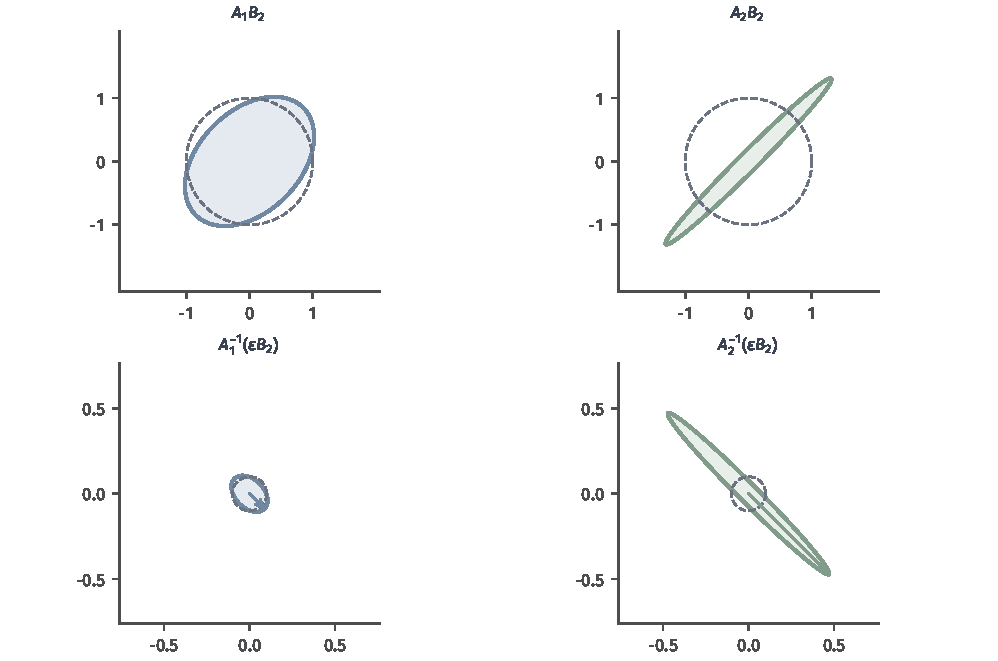
\includegraphics[width=169.0mm]{figures/00-shared/mathematical-preliminaries-upper/02-linear-spaces/matplotlib/ls-condition-number-amplification/ls-condition-number-amplification.pdf}
 \caption{条件数对误差圆盘的放大。灰虚线为单位圆$\lVert\bm z\rVert=1$；左为良态
 $\bm A_1=[[1,0.2],[0.2,1]]$，奇异值$1.20$与$0.80$，$\kappa_2=1.5$，像椭圆接近
 圆；右为病态$\bm A_2=[[1,0.85],[0.85,1]]$，奇异值$1.85$与$0.15$，$\kappa_2\approx12.3$，
 像被拉成细条。半径$\varepsilon=0.1$的误差圆盘（红）最长半轴为$\varepsilon/\sigma_{\min}$：
 良态为$0.125$，病态约$0.67$。}
 \label{fig:ls-condition-number-amplification}
\end{figure*}

条件数看的是方向之间的差异，不是矩阵元素或奇异值的大小。比较$\operatorname{diag}(1,s)$与$s\bm I$（$0<s<1$）：前者的奇异值为$1$与$s$，$\kappa_2=1/s$；后者的奇异值全为$s$，$\kappa_2=1$。

$s\bm I$把每个向量都缩小，数值整体更小，但它对所有方向一视同仁：对任意$\bm x\neq\bm0$，
\[
 \kappa_{\mathrm{rel}}(s\bm I;\bm x)=\frac{s\lVert\bm x\rVert_2}{s\lVert\bm x\rVert_2}=1 ,
\]
相对误差完全不被放大。$\operatorname{diag}(1,s)$只压缩第二个方向，示例~\ref{ex:ls-diagonal-relative-error-basepoints}中的放大正来自两个方向的这种差别。一般地，所有奇异值按同一比例缩放时条件数不变。

条件数也不描述反复作用的长期结果。下面两个矩阵的条件数相同，幂的变化趋势却相反。
\begin{example}[条件数相同而幂的趋势相反]
\label{ex:ls-condition-number-vs-powers}
比较同阶的$2\bm I$与$\tfrac12\bm I$。二者分别把每个方向放大$2$倍和缩小一半，奇异值全为$2$与全为$\tfrac12$，各方向之间没有差别，所以
\[
 \kappa_2(2\bm I)=\frac{2}{2}=1,\qquad
 \kappa_2\bigl(\tfrac12\bm I\bigr)=\frac{1/2}{1/2}=1 .
\]
反复作用时二者却走向相反，前者逐次增长，后者逐次衰减：
\[
 (2\bm I)^k=2^k\bm I,\qquad
 \bigl(\tfrac12\bm I\bigr)^k=2^{-k}\bm I .
\]
条件数只比较最强与最弱方向之比，整体的放大或缩小在比值中被约掉了。
\end{example}
条件数衡量的是一次作用中相对误差的最坏放大，反复作用的长期行为要由谱半径判断（第~\ref{sec:ls-matrix-power-behavior}节），二者不能互相代替。

最后说明本节结论的适用范围。本节始终固定矩阵$\bm A$，只让输入向量带误差，条件数给出的是这种误差在一次线性作用中的最坏放大；它刻画问题本身的敏感性，不评价具体算法。

第~\ref{sec:ls-numerical-sensitivity}节把输出改为方程的解，研究矩阵与右端同时带误差时的完整误差界，并区分数据误差与算法误差；第~\ref{sec:multivariable-inverse-perturbation}节再研究求逆和解映射对矩阵变化的一阶响应。下一节开始改变矩阵本身，分别检查特征值、奇异值和特征子空间。这些输出各有自己的敏感性度量，不能只凭$\kappa_2(\bm A)$判断它们是否敏感。

% 第7章第2节：谱与奇异值的扰动（对称矩阵特征值的扰动，奇异值的扰动与秩判断，特征子空间的扰动，一般方阵的谱敏感性）。

\section{谱与奇异值的扰动}
\label{sec:ls-spectral-sensitivity}
\label{sec:linear-algebra-spectral-stability}
\label{sec:ch06-spectral-stability}

上一节固定矩阵，只让输入向量带误差。实际中矩阵本身也来自数据：协方差矩阵由有限样本估计，系数矩阵经过测量和舍入。设手中的矩阵与真实矩阵相差$\bm E$，我们只知道误差预算$\lVert\bm E\rVert_2\leq\varepsilon$。由手中矩阵算出的特征值、奇异值、秩和特征子空间，哪些结论对真实矩阵仍然可靠？

谱值的大小、矩阵是否接近秩亏、所选子空间的方向，是三种不同的输出，各自需要相应的界与条件。本节先为对称矩阵的每个特征值给出误差区间，并据此判断正负性；再把区间移到奇异值上，检查秩与可逆性；随后研究所选特征子空间的偏转，说明它由谱隙控制；最后说明一般方阵的特征值为什么需要额外的条件。

本节的界都是有限变化界，对任意大小的$\bm E$成立，不需要微分。在可微条件下求所选特征值分支沿指定方向的一阶响应，留给第~\ref{chap:differential-perturbation-analysis}章（第~\ref{sec:multivariable-eigenvalue-differential}节与第~\ref{sec:multivariable-eigenvector-differential}节）。

\subsection{对称矩阵特征值的扰动}
\label{sec:ls-spectral-value-sensitivity}

本小节取实对称矩阵$\bm S\in\mathbb R^{d\times d}$与对称扰动$\bm E$。二者的特征值都是实数，记$\bm S$的特征值为$\lambda_1(\bm S)\geq\cdots\geq\lambda_d(\bm S)$，$\bm S+\bm E$的特征值也按降序记为$\lambda_k(\bm S+\bm E)$，再按同一次序逐个比较，把$\lambda_k(\bm S)$看作$\lambda_k(\bm S+\bm E)$的估计。目标是为每个特征值给出区间，并据此判断正负性和正定性。

图~\ref{fig:ls-perturbation-ellipse}画出一个正定矩阵（图中记为$\bm A$）受扰动前后的二次型椭圆：半轴长微变，主轴微转。半轴长对应特征值，主轴对应特征方向；本小节先处理前者，主轴的转动留到第~\ref{sec:ls-subspace-sensitivity}节。

\begin{figure}[htbp]
 \centering
 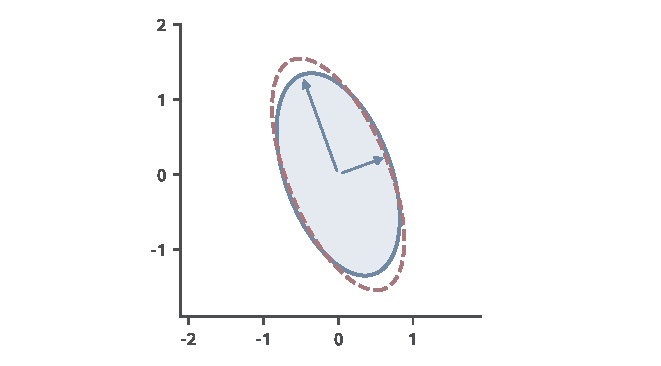
\includegraphics[width=112mm]{figures/00-shared/mathematical-preliminaries-upper/02-linear-spaces/matplotlib/ls-perturbation-ellipse/ls-perturbation-ellipse.pdf}
 \caption{对称矩阵微扰的谱与方向。实线椭圆$\bm x^\top\bm A\bm x=1$对应$\bm A$（特征值$2$与$0.5$，主轴
 方向$20^\circ$），虚线对应$\bm A+\bm E$（$\lVert\bm E\rVert_2\approx0.193$）：轴
 微旋、半轴微变。新特征值约$2.18$与$0.37$，偏移$0.18$、$0.13$均小于
 $\lVert\bm E\rVert_2$，符合Weyl界；未扰动的谱隙$\delta=\lambda_1-\lambda_2=1.5$越大，
 特征方向越不易被微扰转动。}
 \label{fig:ls-perturbation-ellipse}
\end{figure}

\paragraph{有序特征值的比较}

扰动对同一方向上二次型的影响很容易估计：由Cauchy--Schwarz不等式，对任意$\bm x$，
\[
 |\bm x^\top\bm E\bm x|\leq\lVert\bm x\rVert_2\lVert\bm E\bm x\rVert_2\leq\lVert\bm E\rVert_2\lVert\bm x\rVert_2^2 .
\]
所以$\bm S$与$\bm S+\bm E$在同一个单位向量上的二次型值相差不超过$\lVert\bm E\rVert_2$。难点在于把这个逐方向的比较传到第$k$个特征值上：两个矩阵的特征方向一般不同，不能直接拿同一个特征向量比较。

办法是用子空间刻画有序特征值。由谱分解，第$k$个特征值把前$k$个特征方向与后$d-k+1$个特征方向分开，二次型在这两组方向张成的子空间上分别不小于、不大于$\lambda_k$。

\begin{lemma}[特征子空间上的二次型界]
\label{lem:ls-eigen-subspace-quadratic-bounds}
\label{lem:ls-restricted-rayleigh}
设$\bm S\in\mathbb R^{d\times d}$实对称，特征值为$\lambda_1\geq\cdots\geq\lambda_d$，对应的标准正交特征向量为$\bm q_1,\ldots,\bm q_d$。对$1\leq k\leq d$，记$\mathcal V_k=\operatorname{span}\{\bm q_1,\ldots,\bm q_k\}$，$\mathcal W_k=\operatorname{span}\{\bm q_k,\ldots,\bm q_d\}$。则
\[
 \bm x^\top\bm S\bm x\geq\lambda_k\lVert\bm x\rVert_2^2\quad(\bm x\in\mathcal V_k),\qquad
 \bm x^\top\bm S\bm x\leq\lambda_k\lVert\bm x\rVert_2^2\quad(\bm x\in\mathcal W_k),
\]
两式在$\bm x=\bm q_k$时都取等号。
\end{lemma}
\begin{proof}
对$\bm x=\sum_{i\leq k}c_i\bm q_i\in\mathcal V_k$，由二次型展开式~\eqref{eq:matrix-analysis-quadratic-spectral-form}，$\bm x^\top\bm S\bm x=\sum_{i\leq k}\lambda_ic_i^2\geq\lambda_k\sum_{i\leq k}c_i^2=\lambda_k\lVert\bm x\rVert_2^2$，因为$i\leq k$时$\lambda_i\geq\lambda_k$。对$\mathcal W_k$中的向量同理，只是$i\geq k$时$\lambda_i\leq\lambda_k$。取$\bm x=\bm q_k$时只有一项，两式都成为等式。
\end{proof}

两个子空间的维数分别是$k$与$d-k+1$，和为$d+1$，超过了空间的维数。由维数公式，任一$k$维子空间与任一$d-k+1$维子空间的交至少是一维的：
\[
 \dim(\mathcal V\cap\mathcal W)\geq\dim\mathcal V+\dim\mathcal W-d=1 .
\]
这样就能在两个矩阵各自的特征子空间中找到一个公共方向，在这个方向上比较二次型。

\begin{theorem}[Weyl特征值扰动界]
\label{thm:ls-weyl-eigenvalue}
设$\bm S,\bm E\in\mathbb R^{d\times d}$实对称。对每个$k=1,\ldots,d$，按降序配对的特征值满足
\begin{equation}
 |\lambda_k(\bm S+\bm E)-\lambda_k(\bm S)|\leq\lVert\bm E\rVert_2 .
 \label{eq:matrix-analysis-weyl-eigenvalue-perturbation}
\end{equation}
\end{theorem}
\begin{proof}
记$\widetilde{\bm S}=\bm S+\bm E$，$c=\lVert\bm E\rVert_2$。取$\bm S$前$k$个特征向量张成的$\mathcal V_k$，以及$\widetilde{\bm S}$第$k$个到第$d$个特征向量张成的$\widetilde{\mathcal W}_k$。由维数公式，二者有公共的单位向量$\bm x$。对$\bm S$与$\widetilde{\bm S}$分别使用引理~\ref{lem:ls-eigen-subspace-quadratic-bounds}，得
\[
 \lambda_k(\bm S)\leq\bm x^\top\bm S\bm x,\qquad
 \bm x^\top\widetilde{\bm S}\bm x\leq\lambda_k(\widetilde{\bm S}).
\]
又$\bm x^\top\widetilde{\bm S}\bm x=\bm x^\top\bm S\bm x+\bm x^\top\bm E\bm x\geq\bm x^\top\bm S\bm x-c$，三式连起来，
\[
 \lambda_k(\widetilde{\bm S})\geq\bm x^\top\widetilde{\bm S}\bm x\geq\bm x^\top\bm S\bm x-c\geq\lambda_k(\bm S)-c .
\]
交换两个矩阵的角色，把$\bm S=\widetilde{\bm S}+(-\bm E)$看作$\widetilde{\bm S}$的扰动，而$\lVert-\bm E\rVert_2=c$，同样得到$\lambda_k(\bm S)\geq\lambda_k(\widetilde{\bm S})-c$。两式合起来即为结论。
\end{proof}

证明只用了谱分解、维数公式和同一方向上二次型的比较，没有求任何二次型的最大值或最小值。它也不要求特征值彼此分开：重特征值时，$\bm q_k$可以在特征空间中任意选取，引理与证明都不受影响。

\paragraph{最小最大原理}

证明中的论证还给出单个有序特征值的一种不依赖特征向量的刻画。把公共方向的论证用于任意子空间，就得到下面的结论。

\begin{theorem}[Courant--Fischer]
\label{thm:matrix-analysis-courant-fischer}
\label{eq:matrix-analysis-courant-fischer}
设$\bm S\in\mathbb R^{d\times d}$实对称，特征值为$\lambda_1\geq\cdots\geq\lambda_d$。对$k=1,\ldots,d$，
\begin{equation*}
\begin{aligned}
 \lambda_k
 &=\max_{\dim\mathcal V=k}\ \min_{\bm x\in\mathcal V,\lVert\bm x\rVert_2=1}\bm x^\top\bm S\bm x\\
 &=\min_{\dim\mathcal W=d-k+1}\ \max_{\bm x\in\mathcal W,\lVert\bm x\rVert_2=1}\bm x^\top\bm S\bm x .
\end{aligned}
\end{equation*}
\end{theorem}
\begin{proof}
先说明内层的最小值与最大值取得到。设$\mathcal V$是$k$维子空间，$\bm U\in\mathbb R^{d\times k}$的列是它的标准正交基。$\bm x=\bm U\bm y$是$\mathcal V$中的单位向量，当且仅当$\bm y$是$\mathbb R^k$中的单位向量，且$\bm x^\top\bm S\bm x=\bm y^\top\bm M\bm y$，其中$\bm M=\bm U^\top\bm S\bm U$是$k$阶实对称矩阵。对$\bm M$用谱定理与二次型展开式，单位向量上的$\bm y^\top\bm M\bm y$是$\bm M$的特征值的加权平均，最小值与最大值分别是$\bm M$的最小、最大特征值，并在相应的特征向量处取到。

再证第一式。由引理~\ref{lem:ls-eigen-subspace-quadratic-bounds}，$\mathcal V_k$中单位向量的二次型不小于$\lambda_k$，且在$\bm q_k$处等于$\lambda_k$，所以外层的最大值至少为$\lambda_k$。反过来，任一$k$维子空间$\mathcal V$与$\mathcal W_k$有公共的单位向量$\bm x$，它的二次型不超过$\lambda_k$，所以$\mathcal V$上的最小值不超过$\lambda_k$。两方面合起来，外层最大值等于$\lambda_k$，并在$\mathcal V_k$处取到。

第二式交换两组特征向量的角色：$\mathcal W_k$上单位向量的二次型的最大值恰为$\lambda_k$；任一$d-k+1$维子空间$\mathcal W$与$\mathcal V_k$有公共的单位向量，其二次型不小于$\lambda_k$，所以$\mathcal W$上的最大值不小于$\lambda_k$。
\end{proof}

这一定理称为\term{最小最大原理}（min-max principle）。它只涉及子空间与二次型，不要求先知道特征向量；Weyl界也可以由它推出，只需对同一个子空间比较$\bm S$与$\bm S+\bm E$的二次型。$k=1$与$k=d$时，内层只剩一个子空间，结论化为二次型在单位球面上的最大值与最小值；第~\ref{chap:matrix-approximation}章把$\bm x^\top\bm S\bm x/\bm x^\top\bm x$称为Rayleigh商，并从选择最优方向的问题出发研究这两个极值。那里的迹极值汇总$k$个正交方向的贡献，刻画前$k$个特征值之和；最小最大原理刻画的是单个有序特征值。

\paragraph{谱值区间与正定性保证}

由Weyl界，若$\lVert\bm E\rVert_2\leq\varepsilon$，每个真实特征值都落在区间$[\lambda_k(\bm S)-\varepsilon,\lambda_k(\bm S)+\varepsilon]$内。这个绝对误差界不要求特征值彼此分开，单重与重复特征值都适用。但它是绝对误差界：特征值本身接近零时，区间宽度$2\varepsilon$可能与特征值同量级，不能据此宣称相对误差也小。

区间立刻给出特征值符号的判断。若区间不含零，符号由区间确定；若区间含零，当前的误差预算不足以判断符号。例如$\bm S=\operatorname{diag}(1,\varepsilon/2)$，$0<\varepsilon<1$：取$\bm E=\bm0$时第二个特征值为正，取$\bm E=-\varepsilon\bm e_2\bm e_2^\top$时它变为$-\varepsilon/2$，两种扰动都满足预算。正定矩阵沿一条线段变化时，还可以得到对整条线段一致的下界。
\begin{theorem}[特征值的符号与正定性保持]
\label{thm:ls-eigenvalue-sign-definiteness}
设$\bm S,\bm E\in\mathbb R^{d\times d}$实对称，$\lVert\bm E\rVert_2\leq\varepsilon$。
\begin{enumerate}
 \item 若$\lambda_k(\bm S)>\varepsilon$，则$\lambda_k(\bm S+\bm E)>0$；若$\lambda_k(\bm S)<-\varepsilon$，则$\lambda_k(\bm S+\bm E)<0$。
 \item 若$\bm S$正定且$\varepsilon<\lambda_{\min}(\bm S)$，则对一切$t\in[0,1]$，
 \[
  \lambda_{\min}(\bm S+t\bm E)\geq\lambda_{\min}(\bm S)-\varepsilon>0 ,
 \]
 从而线段$\{\bm S+t\bm E:0\leq t\leq1\}$上的矩阵都正定。
\end{enumerate}
\end{theorem}
\begin{proof}
第1条：由定理~\ref{thm:ls-weyl-eigenvalue}，$\lambda_k(\bm S+\bm E)\geq\lambda_k(\bm S)-\varepsilon>0$；负号情形同理，$\lambda_k(\bm S+\bm E)\leq\lambda_k(\bm S)+\varepsilon<0$。第2条：对$t\in[0,1]$，$t\bm E$对称且$\lVert t\bm E\rVert_2=t\lVert\bm E\rVert_2\leq\varepsilon$。对最小特征值$\lambda_d$应用定理~\ref{thm:ls-weyl-eigenvalue}，得$\lambda_{\min}(\bm S+t\bm E)\geq\lambda_{\min}(\bm S)-\varepsilon>0$。实对称矩阵的特征值全为正时，由二次型展开式~\eqref{eq:matrix-analysis-quadratic-spectral-form}，它是正定的。
\end{proof}
第2条的下界$\lambda_{\min}(\bm S)-\varepsilon$与$t$无关。后文对正定矩阵求逆、开方或取对数时，常需确认整条线段都留在这些运算的定义域内，并且离定义域边界有一致的距离，例如第~\ref{sec:multivariable-logdet-perturbation}节估计对数行列式的变化；这个下界正好提供这一保证。

最后用一个例子检查界的精确程度，并看到有限变化界与可微性是两回事。
\begin{example}[重根处的最大特征值]
\label{ex:ls-weyl-double-root}
取$\bm S(t)=\operatorname{diag}(t,-t)$，$t\in\mathbb R$，从重根$\bm S(0)=\bm0$出发看最大特征值怎样移动。$\bm S(0)$的特征值$0$是二重根；$t\neq0$时两个特征值$\pm t$分开，排序后的最大特征值为$|t|$。

它相对于$\bm S(0)$的变化是$|t|$，恰好等于$\lVert\bm S(t)-\bm S(0)\rVert_2=|t|$，所以界~\eqref{eq:matrix-analysis-weyl-eigenvalue-perturbation}在这里取等号，不能再改进；同时也说明重根并不妨碍有限的绝对误差界。但有界的变化不等于光滑的变化：$|t|$在$t=0$处左导数为$-1$、右导数为$1$，排序后的最大特征值在重根处没有双侧导数。原因是$t$变号时，最大特征值从$t$这一支换到$-t$那一支。
\end{example}
第~\ref{sec:multivariable-local-condition-number}节再用这个例子区分有限敏感性与可微性；第~\ref{sec:multivariable-eigenvalue-differential}节在特征值简单的条件下，另行研究所选分支的一阶响应。

\subsection{奇异值的扰动与秩判断}
\label{sec:ls-singular-value-sensitivity}

秩、可逆性与最佳低秩逼近的误差都由奇异值决定。本小节先把上一小节的特征值区间移到奇异值上，再据此判断哪些关于秩的结论在误差预算下仍然可靠。

\paragraph{奇异值的误差区间}

长方矩阵没有特征值，不能直接使用Weyl界。办法是把它放进一个对称矩阵，使后者的特征值恰好包含原矩阵的奇异值。对$\bm A\in\mathbb R^{m\times n}$，记$p=\min(m,n)$，奇异值为$\sigma_1(\bm A)\geq\cdots\geq\sigma_p(\bm A)\geq0$，定义$(m+n)$阶对称增广矩阵
\[
 \bm H(\bm A)=\begin{bmatrix}\bm0&\bm A\\\bm A^\top&\bm0\end{bmatrix},
\]

\begin{lemma}[对称增广矩阵的谱]
\label{lem:ls-symmetric-augmentation-spectrum}
$\bm H(\bm A)$的特征值为$\pm\sigma_1(\bm A)$、$\ldots$、$\pm\sigma_p(\bm A)$，以及$|m-n|$个零。特别地，按降序排列时它的前$p$个特征值依次为$\sigma_1(\bm A),\ldots,\sigma_p(\bm A)$；并且$\lVert\bm H(\bm A)\rVert_2=\lVert\bm A\rVert_2$。
\end{lemma}
\begin{proof}
由定理~\ref{thm:ls-svd-existence}，取完整的SVD $\bm A=\bm U\bm\Sigma\bm V^\top$，列向量为$\bm u_1,\ldots,\bm u_m$与$\bm v_1,\ldots,\bm v_n$。对$i\leq p$，有$\bm A\bm v_i=\sigma_i\bm u_i$与$\bm A^\top\bm u_i=\bm V\bm\Sigma^\top\bm e_i=\sigma_i\bm v_i$。令
\[
 \bm w_i^{\pm}=\frac1{\sqrt2}\begin{bmatrix}\bm u_i\\\pm\bm v_i\end{bmatrix},
\]
用$(\bm a;\bm b)$表示把$\bm a$、$\bm b$上下拼接成的列向量，则
\[
 \bm H(\bm A)\bm w_i^{\pm}=\tfrac1{\sqrt2}(\pm\bm A\bm v_i;\bm A^\top\bm u_i)=\tfrac1{\sqrt2}(\pm\sigma_i\bm u_i;\sigma_i\bm v_i)=\pm\sigma_i\bm w_i^{\pm}.
\]
若$m>n$，对$j>n$，$\bm\Sigma^\top$的第$j$列为零，故$\bm A^\top\bm u_j=\bm0$，向量$(\bm u_j;\bm0)$是特征值$0$的特征向量；若$n>m$，对$j>m$有$\bm A\bm v_j=\bm0$，向量$(\bm0;\bm v_j)$是特征值$0$的特征向量。这$2p+|m-n|=m+n$个向量两两正交且长度为$1$：由$\bm u_i$、$\bm v_i$各自标准正交，$\bm w_i^{\pm}$与$\bm w_j^{\pm}$的内积为$\tfrac12(\bm u_i^\top\bm u_j\pm\bm v_i^\top\bm v_j)$，两者符号相同时取正号、相反时取负号，所以$i\neq j$时为零，$i=j$而符号相反时为$\tfrac12(1-1)=0$，符号相同时为$1$；补充的向量$(\bm u_j;\bm0)$或$(\bm0;\bm v_j)$只含$j>p$的分量，与所有$\bm w_i^{\pm}$及彼此都正交。所以它们构成$\bm H(\bm A)$的标准正交特征基，列出了全部特征值（计重数）。$\sigma_i\geq0\geq-\sigma_j$，所以降序排列时前$p$个是$\sigma_1,\ldots,\sigma_p$。

最后，对$\bm z=(\bm y;\bm x)$，$\bm H(\bm A)\bm z=(\bm A\bm x;\bm A^\top\bm y)$。$\bm A^\top$与$\bm A$有相同的非零奇异值，所以$\lVert\bm A^\top\rVert_2=\lVert\bm A\rVert_2$，于是
\[
 \begin{aligned}
 \lVert\bm H(\bm A)\bm z\rVert_2^2
 &=\lVert\bm A\bm x\rVert_2^2+\lVert\bm A^\top\bm y\rVert_2^2\\
 &\leq\lVert\bm A\rVert_2^2\bigl(\lVert\bm x\rVert_2^2+\lVert\bm y\rVert_2^2\bigr)
 =\lVert\bm A\rVert_2^2\lVert\bm z\rVert_2^2 ,
 \end{aligned}
\]
而$\bm z=\bm w_1^+$时$\lVert\bm H(\bm A)\bm z\rVert_2=\sigma_1=\lVert\bm A\rVert_2$，故$\lVert\bm H(\bm A)\rVert_2=\lVert\bm A\rVert_2$。
\end{proof}

\begin{theorem}[奇异值的Weyl界]
\label{thm:ls-weyl-singular-value}
设$\bm A,\bm E\in\mathbb R^{m\times n}$，$p=\min(m,n)$。对$i=1,\ldots,p$，
\begin{equation}
 |\sigma_i(\bm A+\bm E)-\sigma_i(\bm A)|\leq\lVert\bm E\rVert_2 .
 \label{eq:matrix-analysis-singular-value-perturbation}
\end{equation}
\end{theorem}
\begin{proof}
增广是线性的：$\bm H(\bm A+\bm E)=\bm H(\bm A)+\bm H(\bm E)$，三者都实对称。对$\bm H(\bm A)$与扰动$\bm H(\bm E)$应用定理~\ref{thm:ls-weyl-eigenvalue}，第$i$个特征值的变化不超过$\lVert\bm H(\bm E)\rVert_2$。由引理~\ref{lem:ls-symmetric-augmentation-spectrum}，$i\leq p$时第$i$个特征值就是第$i$个奇异值，且$\lVert\bm H(\bm E)\rVert_2=\lVert\bm E\rVert_2$。
\end{proof}
奇异值非负，所以在误差预算$\lVert\bm E\rVert_2\leq\varepsilon$下，真实的第$i$个奇异值落在非负区间$[\max(0,\sigma_i(\bm A)-\varepsilon),\ \sigma_i(\bm A)+\varepsilon]$内。

最佳低秩逼近的误差也随之受控。第~\ref{chap:matrix-approximation}章将证明（定理~\ref{thm:matrix-analysis-best-low-rank}），对$0\leq k<p$，秩不超过$k$的矩阵中，与$\bm A$的最小谱范数距离为$\sigma_{k+1}(\bm A)$。把定理~\ref{thm:ls-weyl-singular-value}用于$i=k+1$，扰动前后这个最优误差之差不超过$\varepsilon$。要注意，这只说明最优误差的数值稳定；取得最优误差的低秩矩阵及其所用的奇异方向是否同样稳定，是另一个问题，留到下一小节。

\paragraph{秩保证与可逆性的边界}

奇异值区间不含零，就能保证相应的奇异值为正，从而给出秩的下界。
\begin{theorem}[由奇异值保证秩]
\label{thm:ls-singular-value-rank-guarantee}
设$\bm A,\bm E\in\mathbb R^{m\times n}$，$\lVert\bm E\rVert_2\leq\varepsilon$，$1\leq k\leq\min(m,n)$。若$\sigma_k(\bm A)>\varepsilon$，则$\operatorname{rank}(\bm A+\bm E)\geq k$。特别地，$m\geq n$且$\sigma_n(\bm A)>\varepsilon$时，$\bm A+\bm E$满列秩。
\end{theorem}
\begin{proof}
由定理~\ref{thm:ls-weyl-singular-value}，$\sigma_k(\bm A+\bm E)\geq\sigma_k(\bm A)-\varepsilon>0$，而奇异值降序排列，所以$\bm A+\bm E$至少有$k$个正奇异值。由定理~\ref{thm:ls-svd-existence}，正奇异值的个数等于秩。
\end{proof}
反方向的结论不成立：$\sigma_k(\bm A)\leq\varepsilon$只表示区间$[\max(0,\sigma_k(\bm A)-\varepsilon),\sigma_k(\bm A)+\varepsilon]$包含零，无法排除真实矩阵的第$k$个奇异值为零，但也不能由此断言真实矩阵秩亏。

这里要区分两种秩。精确秩对扰动不连续：$\operatorname{diag}(1,0)+t\bm e_2\bm e_2^\top$对每个$t\neq0$都可逆，秩为$2$，$t=0$时秩突然降为$1$，无论$|t|$多小。所以对带误差的矩阵，追问精确秩没有意义；可靠的是给定误差预算下的有效秩，即定理保证的下界“大于$\varepsilon$的奇异值个数”。本小节只给出由误差预算能够保证的结论；实际计算中怎样选取阈值、把大于阈值的奇异值个数作为数值秩，在第~\ref{sec:ls-pseudoinverse-rank-change}节结合求解任务讨论。

对可逆方阵，同样的想法回答：最小要多大的扰动，才能使它变成奇异矩阵？
\begin{theorem}[到奇异矩阵的距离]
\label{thm:ls-distance-to-singularity}
设$\bm A\in\mathbb R^{n\times n}$可逆，奇异值为$\sigma_1\geq\cdots\geq\sigma_n>0$，$\bm u_n$、$\bm v_n$是与$\sigma_n$对应的单位左、右奇异向量。则
\[
 \min\{\lVert\bm E\rVert_2:\bm A+\bm E\text{ 奇异}\}=\sigma_n(\bm A),
\]
最小值在$\bm E_*=-\sigma_n\bm u_n\bm v_n^\top$处取到。相对于$\lVert\bm A\rVert_2$，这个距离为
\[
 \frac{\sigma_n(\bm A)}{\lVert\bm A\rVert_2}=\frac1{\kappa_2(\bm A)} .
\]
\end{theorem}
\begin{proof}
分两步证明：较小的扰动保持可逆，而$\bm E_*$恰好使矩阵奇异。

下界：设$\lVert\bm E\rVert_2<\sigma_n$。对任意$\bm x\neq\bm0$，由定理~\ref{thm:matrix-analysis-condition-number-bound}证明中的估计$\lVert\bm A\bm x\rVert_2\geq\sigma_n\lVert\bm x\rVert_2$，
\[
 \begin{aligned}
 \lVert(\bm A+\bm E)\bm x\rVert_2
 &\geq\lVert\bm A\bm x\rVert_2-\lVert\bm E\bm x\rVert_2\\
 &\geq(\sigma_n-\lVert\bm E\rVert_2)\lVert\bm x\rVert_2>0 ,
 \end{aligned}
\]
所以$\bm A+\bm E$的零空间只含零向量，它可逆。可达：对任意$\bm x$，$\lVert\bm u_n\bm v_n^\top\bm x\rVert_2=|\bm v_n^\top\bm x|\leq\lVert\bm x\rVert_2$，且$\bm x=\bm v_n$时取等号，故$\lVert\bm E_*\rVert_2=\sigma_n$；又$(\bm A+\bm E_*)\bm v_n=\sigma_n\bm u_n-\sigma_n\bm u_n=\bm0$，所以$\bm A+\bm E_*$奇异。相对距离由$\lVert\bm A\rVert_2=\sigma_1$与$\kappa_2(\bm A)=\sigma_1/\sigma_n$得到。
\end{proof}
$n$阶方阵奇异，当且仅当它的秩不超过$n-1$，所以这个定理也是第~\ref{chap:matrix-approximation}章最佳低秩逼近在$k=n-1$时的特例；这里的直接证明只用到最小奇异值的下界。
这为上一节的矩阵条件数提供了另一种解释：$\kappa_2(\bm A)$越大，按相对尺度计，$\bm A$离奇异矩阵越近。这个结论的条件是允许任意的谱范数扰动；若扰动必须保持某种结构，例如对称或稀疏，可选的扰动变少，本定理只给出距离的下界，相应的距离需要另行分析。还要注意，扰动超过$\sigma_n$并不意味着每个这样的扰动都使矩阵奇异，例如$\bm E=\bm A$的范数为$\sigma_1\geq\sigma_n$，而$\bm A+\bm E=2\bm A$仍然可逆。

\begin{example}[对角矩阵的可逆性边界]
\label{ex:ls-diagonal-distance-to-singularity}
回到上一节的$\bm A=\operatorname{diag}(1,s)$，$0<s<1$。它的奇异值为$1$与$s$，$\kappa_2(\bm A)=1/s$。由定理~\ref{thm:ls-distance-to-singularity}，误差预算$\varepsilon<s$时可以保证$\bm A+\bm E$可逆。这个门槛不能再放宽：$\bm E=-s\bm e_2\bm e_2^\top$的范数恰为$s$，它把第二个对角元抵消掉，使$\bm A$变成奇异的$\operatorname{diag}(1,0)$。按相对尺度，这个距离是$s/1=1/\kappa_2(\bm A)$；$s$越小，条件数越大，$\bm A$离奇异矩阵也越近。
\end{example}
在这个例子中，$s$很小时矩阵离奇异很近，但它的第一奇异方向$\bm e_1$并不因此变得不稳定。下一小节将说明，保留第一奇异方向的稳定性由截断处的间隙$\sigma_1-\sigma_2=1-s$决定，而可逆性的边界由最小奇异值$s$决定，二者不能互相替代。

\subsection{特征子空间的扰动}
\label{sec:ls-subspace-sensitivity}

即使特征值的绝对误差很小，按这些特征值选出的方向也可能变化很大。本小节研究：在给定的误差预算下，原来选出的特征子空间能偏转多少。先建立一种不依赖基的选择的子空间距离，再检查目标特征值组与其余特征值之间的间隔。

\paragraph{子空间的距离}

比较特征向量时，比较对象应是子空间本身。特征向量可以变号；特征值重复时，特征空间内部还可以任意换标准正交基，这些都不改变子空间，所以单个基向量的变化不能当作子空间的误差。图~\ref{fig:ls-principal-angles-subspaces}从两条过原点的直线看起：两直线的夹角与方向向量的选取无关；把一条直线的单位方向向量投影到另一条上，投影不掉的部分长度为$\sin\theta$。

\begin{figure}[htbp]
 \centering
 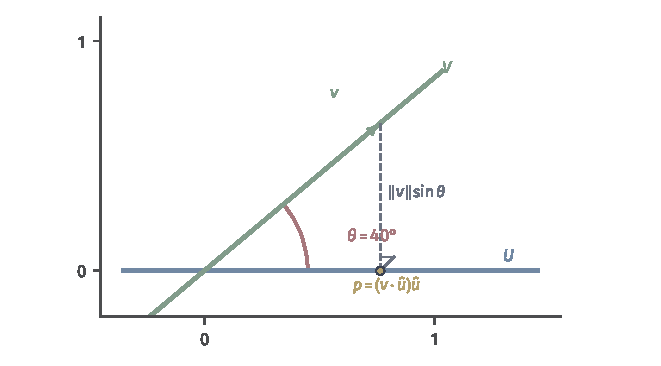
\includegraphics[width=112mm]{figures/00-shared/mathematical-preliminaries-upper/02-linear-spaces/matplotlib/ls-principal-angles-subspaces/ls-principal-angles-subspaces.pdf}
 \caption{两条直线子空间的主夹角。蓝线为$\bm U$、绿线为$\bm V$，红弧为主夹角
 $\theta=40^\circ$；黄点$\bm p$是$\bm v$在$\bm U$上的正交投影，灰虚线为投影
 垂线。$\cos40^\circ\approx0.766$、$\sin40^\circ\approx0.643$，残差长度
 $\lVert\bm v\rVert\sin\theta$即投影不掉的分量。}
 \label{fig:ls-principal-angles-subspaces}
\end{figure}

对一维子空间，若$\bm q,\widetilde{\bm q}$是单位方向向量，则$|\bm q^\top\widetilde{\bm q}|=\cos\theta$。高维子空间之间有多个夹角，由交叉内积矩阵的奇异值给出。
\begin{definition}[主夹角]
\label{def:matrix-analysis-principal-angles}
设$\bm Q,\widetilde{\bm Q}\in\mathbb R^{d\times r}$列标准正交，分别张成$r$维子空间。交叉矩阵$\bm Q^\top\widetilde{\bm Q}$的奇异值记为$\cos\theta_1\geq\dots\geq\cos\theta_r$，$0\leq\theta_1\leq\cdots\leq\theta_r\leq\pi/2$，这些$\theta_i$称为两个子空间的\term{主夹角}（principal angles）。
\end{definition}
这些奇异值都在$[0,1]$内，因为$\lVert\bm Q^\top\widetilde{\bm Q}\rVert_2\leq\lVert\bm Q\rVert_2\lVert\widetilde{\bm Q}\rVert_2=1$，所以$\theta_i$有定义。换基相当于把$\bm Q$、$\widetilde{\bm Q}$分别右乘$r$阶正交矩阵$\bm R$、$\widetilde{\bm R}$，交叉矩阵变为$\bm R^\top(\bm Q^\top\widetilde{\bm Q})\widetilde{\bm R}$，奇异值不变，所以主夹角只依赖两个子空间。最大主夹角$\theta_r$记为$\theta_{\max}$。

主夹角的正弦度量一个子空间伸出另一个子空间的部分，它们也可以直接读出，并与正交投影之差联系起来。设$\widetilde{\bm Q}_\perp\in\mathbb R^{d\times(d-r)}$的列是$\widetilde{\bm Q}$列空间正交补的标准正交基，记
\[
 \bm C=\widetilde{\bm Q}^\top\bm Q,\qquad\bm X=\widetilde{\bm Q}_\perp^\top\bm Q ,
\]
再记两个子空间上的正交投影为$\bm P=\bm Q\bm Q^\top$、$\widetilde{\bm P}=\widetilde{\bm Q}\widetilde{\bm Q}^\top$，它们与基的选取无关。
\begin{theorem}[主夹角的正弦与投影之差]
\label{thm:ls-principal-angle-projection}
在上述记号下，$\bm X^\top\bm X=\bm I-\bm C^\top\bm C$，其特征值为$\sin^2\theta_1,\ldots,\sin^2\theta_r$，并且
\[
 \tfrac12\lVert\bm P-\widetilde{\bm P}\rVert_{\mathrm F}^2=\sum_{i=1}^r\sin^2\theta_i=\lVert\bm X\rVert_{\mathrm F}^2 .
\]
\end{theorem}
\begin{proof}
$[\widetilde{\bm Q},\widetilde{\bm Q}_\perp]$是正交矩阵，所以对任意$\bm a\in\mathbb R^r$，把$\bm Q\bm a$分解到$\widetilde{\bm Q}$的列空间与其正交补，由勾股定理，
\[
 \lVert\bm C\bm a\rVert_2^2+\lVert\bm X\bm a\rVert_2^2=\lVert\bm Q\bm a\rVert_2^2=\lVert\bm a\rVert_2^2 .
\]
即对称矩阵$\bm X^\top\bm X$与$\bm I-\bm C^\top\bm C$的二次型处处相等。对称矩阵由其二次型唯一确定（用$\bm a+\bm b$与$\bm a-\bm b$的二次型之差可以读出$\bm a^\top\bm M\bm b$），所以$\bm X^\top\bm X=\bm I-\bm C^\top\bm C$。$\bm C$是交叉矩阵$\bm Q^\top\widetilde{\bm Q}$的转置，$\bm C^\top\bm C$的特征值是$\cos^2\theta_i$，所以$\bm X^\top\bm X$的特征值是$1-\cos^2\theta_i=\sin^2\theta_i$，且$\lVert\bm X\rVert_{\mathrm F}^2=\operatorname{tr}(\bm X^\top\bm X)=\sum_i\sin^2\theta_i$。

再算投影之差。$\bm P$、$\widetilde{\bm P}$对称且$\bm P^2=\bm P$、$\widetilde{\bm P}^2=\widetilde{\bm P}$，$\operatorname{tr}\bm P=\operatorname{tr}(\bm Q^\top\bm Q)=r$，同样$\operatorname{tr}\widetilde{\bm P}=r$。于是
\[
 \begin{aligned}
 \lVert\bm P-\widetilde{\bm P}\rVert_{\mathrm F}^2
 &=\operatorname{tr}\bigl((\bm P-\widetilde{\bm P})^2\bigr)\\
 &=\operatorname{tr}\bm P-2\operatorname{tr}(\bm P\widetilde{\bm P})+\operatorname{tr}\widetilde{\bm P}\\
 &=2r-2\operatorname{tr}(\bm P\widetilde{\bm P}).
 \end{aligned}
\]
由迹的循环性，$\operatorname{tr}(\bm P\widetilde{\bm P})=\operatorname{tr}(\widetilde{\bm Q}^\top\bm Q\bm Q^\top\widetilde{\bm Q})=\lVert\bm Q^\top\widetilde{\bm Q}\rVert_{\mathrm F}^2=\sum_i\cos^2\theta_i$，代入得$\lVert\bm P-\widetilde{\bm P}\rVert_{\mathrm F}^2=2\sum_i(1-\cos^2\theta_i)=2\sum_i\sin^2\theta_i$。
\end{proof}
Frobenius范数汇总了所有主夹角，反映整体偏转。只关心最坏的那个方向时，用谱范数，它恰好读出最大主夹角。
\begin{theorem}[投影之差的谱范数]
\label{thm:ls-projection-spectral-distance}
在定理~\ref{thm:ls-principal-angle-projection}的记号下，
\[
 \lVert\bm P-\widetilde{\bm P}\rVert_2=\lVert\bm X\rVert_2=\sin\theta_{\max}.
\]
\end{theorem}
\begin{proof}
由定理~\ref{thm:ls-principal-angle-projection}，$\bm X^\top\bm X$的最大特征值是$\sin^2\theta_{\max}$，所以$\lVert\bm X\rVert_2=\sin\theta_{\max}$。

再设$\bm Q_\perp\in\mathbb R^{d\times(d-r)}$的列是$\bm Q$列空间正交补的标准正交基，于是$\bm I-\bm P=\bm Q_\perp\bm Q_\perp^\top$、$\bm I-\widetilde{\bm P}=\widetilde{\bm Q}_\perp\widetilde{\bm Q}_\perp^\top$。先说明两个算子范数。列标准正交的矩阵保持长度，行标准正交的矩阵不增加长度，并在其行空间上保持长度，所以
\[
 \lVert(\bm I-\widetilde{\bm P})\bm P\rVert_2
 =\lVert\widetilde{\bm Q}_\perp(\widetilde{\bm Q}_\perp^\top\bm Q)\bm Q^\top\rVert_2
 =\lVert\bm X\rVert_2 .
\]
同理$\lVert(\bm I-\bm P)\widetilde{\bm P}\rVert_2=\lVert\bm Q_\perp^\top\widetilde{\bm Q}\rVert_2$。把定理~\ref{thm:ls-principal-angle-projection}中两个子空间的角色交换，交叉矩阵变为$\widetilde{\bm Q}^\top\bm Q$，它与原交叉矩阵互为转置，奇异值相同，所以$\bm Q_\perp^\top\widetilde{\bm Q}$的最大奇异值同样是$\sin\theta_{\max}$。

上界：直接展开可验证
\[
 \bm P-\widetilde{\bm P}=\bm P(\bm I-\widetilde{\bm P})-(\bm I-\bm P)\widetilde{\bm P}.
\]
对任意$\bm z$，右端第一项落在$\bm Q$的列空间中，第二项落在其正交补中，由勾股定理，
\[
 \begin{aligned}
 \lVert(\bm P-\widetilde{\bm P})\bm z\rVert_2^2
 &=\lVert\bm P(\bm I-\widetilde{\bm P})\bm z\rVert_2^2+\lVert(\bm I-\bm P)\widetilde{\bm P}\bm z\rVert_2^2\\
 &\leq\sin^2\theta_{\max}\bigl(\lVert(\bm I-\widetilde{\bm P})\bm z\rVert_2^2+\lVert\widetilde{\bm P}\bm z\rVert_2^2\bigr)\\
 &=\sin^2\theta_{\max}\lVert\bm z\rVert_2^2 .
 \end{aligned}
\]
这里第二行用到$\bm P(\bm I-\widetilde{\bm P})=\bigl((\bm I-\widetilde{\bm P})\bm P\bigr)^\top$，转置不改变谱范数，并对两项分别使用上面的范数等式；第三行再用勾股定理。

下界：取单位向量$\bm a\in\mathbb R^r$使$\lVert\bm X\bm a\rVert_2=\lVert\bm X\rVert_2$（取$\bm X$的第一右奇异向量），令$\bm z=\bm Q\bm a$，则$\lVert\bm z\rVert_2=1$，$\bm P\bm z=\bm z$，
\[
 (\bm P-\widetilde{\bm P})\bm z=(\bm I-\widetilde{\bm P})\bm Q\bm a=\widetilde{\bm Q}_\perp\bm X\bm a ,
\]
长度为$\lVert\bm X\bm a\rVert_2=\sin\theta_{\max}$。两方面合起来即得结论。
\end{proof}

\paragraph{谱隙控制的偏转界}

现在比较特征子空间。设$\bm S$、$\widetilde{\bm S}=\bm S+\bm E\in\mathbb R^{d\times d}$实对称，取$1\leq k<d$，比较两者前$k$个特征值对应的子空间。要使比较有意义，原矩阵的目标特征值组必须与其余特征值分开：设截断处的\term{谱隙}（spectral gap）
\[
 \delta=\lambda_k(\bm S)-\lambda_{k+1}(\bm S)>0 ,
\]
这时$\bm S$前$k$个特征值对应的特征子空间是唯一确定的$k$维子空间。若误差预算满足$\lVert\bm E\rVert_2\leq\varepsilon<\delta/2$，由Weyl界，
\[
 \lambda_k(\widetilde{\bm S})\geq\lambda_k(\bm S)-\varepsilon>\lambda_{k+1}(\bm S)+\varepsilon\geq\lambda_{k+1}(\widetilde{\bm S}),
\]
扰动后截断处仍然严格分开，$\widetilde{\bm S}$前$k$个特征值的特征子空间也唯一确定，两者都是$k$维，可以用主夹角比较。

下面的论证用到的是交叉谱间隔
\[
 \gamma=\lambda_k(\bm S)-\lambda_{k+1}(\widetilde{\bm S}),
\]
即原目标组的最小特征值与扰动后其余特征值的最大者之差。由Weyl界$\lambda_{k+1}(\widetilde{\bm S})\leq\lambda_{k+1}(\bm S)+\varepsilon$，得$\gamma\geq\delta-\varepsilon>0$。

记$\bm Q\in\mathbb R^{d\times k}$的列是$\bm S$前$k$个特征值的标准正交特征向量，$\bm\Lambda_1=\operatorname{diag}(\lambda_1(\bm S),\ldots,\lambda_k(\bm S))$；$\widetilde{\bm Q}$的列是$\widetilde{\bm S}$前$k$个特征值的标准正交特征向量，$\widetilde{\bm Q}_\perp$的列是其余的标准正交特征向量，对应特征值组成对角矩阵$\widetilde{\bm\Lambda}_2=\operatorname{diag}(\lambda_{k+1}(\widetilde{\bm S}),\ldots,\lambda_d(\widetilde{\bm S}))$。令$\bm X=\widetilde{\bm Q}_\perp^\top\bm Q$，由定理~\ref{thm:ls-principal-angle-projection}，它的Frobenius范数平方就是两个子空间主夹角正弦的平方和。

\begin{theorem}[特征子空间偏转的Frobenius界]
\label{thm:ls-gap-subspace-frobenius}
在上述记号下，若$\gamma=\lambda_k(\bm S)-\lambda_{k+1}(\widetilde{\bm S})>0$，则$\bm Q$与$\widetilde{\bm Q}$张成的子空间的主夹角$\theta_1,\ldots,\theta_k$满足
\[
 \begin{aligned}
 \Bigl(\sum_{i=1}^k\sin^2\theta_i\Bigr)^{1/2}
 &=\lVert\bm X\rVert_{\mathrm F}\\
 &\leq\frac{\lVert\widetilde{\bm Q}_\perp^\top\bm E\bm Q\rVert_{\mathrm F}}{\gamma}
 \leq\frac{\lVert\bm E\bm Q\rVert_{\mathrm F}}{\gamma}.
 \end{aligned}
\]
\end{theorem}
\begin{proof}
由特征关系$\widetilde{\bm Q}_\perp^\top\widetilde{\bm S}=\widetilde{\bm\Lambda}_2\widetilde{\bm Q}_\perp^\top$（对$\widetilde{\bm S}\widetilde{\bm Q}_\perp=\widetilde{\bm Q}_\perp\widetilde{\bm\Lambda}_2$取转置）右乘$\bm Q$，又由$\bm S\bm Q=\bm Q\bm\Lambda_1$左乘$\widetilde{\bm Q}_\perp^\top$，两式相减，并用$\widetilde{\bm S}-\bm S=\bm E$，得
\[
 \widetilde{\bm\Lambda}_2\bm X-\bm X\bm\Lambda_1=\widetilde{\bm Q}_\perp^\top\bm E\bm Q .
\]
这是关于$\bm X$的线性方程，两侧的系数矩阵都是对角的，可以逐元素读出。把$\bm X$的行用$j=k+1,\ldots,d$编号、列用$i=1,\ldots,k$编号，第$(j,i)$元满足
\[
 \bigl(\lambda_j(\widetilde{\bm S})-\lambda_i(\bm S)\bigr)X_{j,i}=(\widetilde{\bm Q}_\perp^\top\bm E\bm Q)_{j,i}.
\]
由降序，$i\leq k<j$时$\lambda_i(\bm S)-\lambda_j(\widetilde{\bm S})\geq\lambda_k(\bm S)-\lambda_{k+1}(\widetilde{\bm S})=\gamma>0$，所以$|X_{j,i}|\leq|(\widetilde{\bm Q}_\perp^\top\bm E\bm Q)_{j,i}|/\gamma$。逐元素平方求和，得第一个不等式。$\widetilde{\bm Q}_\perp^\top$的行标准正交，对任意向量$\bm m$有$\lVert\widetilde{\bm Q}_\perp^\top\bm m\rVert_2\leq\lVert\bm m\rVert_2$，按列应用于$\bm E\bm Q$即得第二个不等式。等式部分来自定理~\ref{thm:ls-principal-angle-projection}。
\end{proof}
证明中出现的方程同时含有左乘和右乘未知矩阵的两项，这类方程称为Sylvester方程，第~\ref{sec:ls-matrix-equations}节专门研究它；这里两侧系数都是对角矩阵，逐元素相除就够了。由$\lVert\bm E\bm Q\rVert_{\mathrm F}\leq\sqrt k\,\lVert\bm E\rVert_2$，右端不超过$\sqrt k\,\lVert\bm E\rVert_2/\gamma$。

对谱范数，即最大主夹角，也有同型的结论。它不是上面Frobenius估计的直接推论：由Frobenius界只能得到带因子$\sqrt k$的估计。去掉这个因子要换一种读法：不逐元素相除，而是用$\bm X$的最大奇异方向从两侧检验同一个矩阵方程。
\begin{theorem}[Davis--Kahan谱隙界]
\label{thm:ls-davis-kahan}
在定理~\ref{thm:ls-gap-subspace-frobenius}的条件下，
\begin{equation}
 \lVert\widetilde{\bm P}-\bm P\rVert_2=\sin\theta_{\max}
 \leq\frac{\lVert\bm E\bm Q\rVert_2}{\gamma}\leq\frac{\lVert\bm E\rVert_2}{\gamma}.
 \label{eq:matrix-analysis-eigenvector-gap-bound}
\end{equation}
\end{theorem}
\begin{proof}
由定理~\ref{thm:ls-projection-spectral-distance}，$\lVert\widetilde{\bm P}-\bm P\rVert_2=\sin\theta_{\max}=\lVert\bm X\rVert_2$，记$s=\lVert\bm X\rVert_2$。$s=0$时结论成立，下设$s>0$。取$\bm X$的第一右、左奇异向量$\bm a\in\mathbb R^k$、$\bm b\in\mathbb R^{d-k}$，它们是单位向量，满足$\bm X\bm a=s\bm b$、$\bm X^\top\bm b=s\bm a$。用$\bm b^\top$左乘、$\bm a$右乘定理~\ref{thm:ls-gap-subspace-frobenius}证明中的方程$\widetilde{\bm\Lambda}_2\bm X-\bm X\bm\Lambda_1=\widetilde{\bm Q}_\perp^\top\bm E\bm Q$，左端为
\[
 \begin{aligned}
 &\bm b^\top\widetilde{\bm\Lambda}_2(\bm X\bm a)-(\bm X^\top\bm b)^\top\bm\Lambda_1\bm a\\
 &\quad=s\bigl(\bm b^\top\widetilde{\bm\Lambda}_2\bm b-\bm a^\top\bm\Lambda_1\bm a\bigr).
 \end{aligned}
\]
$\bm\Lambda_1$的对角元都不小于$\lambda_k(\bm S)$，$\bm a$是单位向量，所以
\[
 \bm a^\top\bm\Lambda_1\bm a=\sum_i\lambda_i(\bm S)a_i^2\geq\lambda_k(\bm S);
\]
同理$\bm b^\top\widetilde{\bm\Lambda}_2\bm b\leq\lambda_{k+1}(\widetilde{\bm S})$。于是左端的绝对值至少为$s\gamma$。右端的绝对值满足
\[
 |\bm b^\top\widetilde{\bm Q}_\perp^\top\bm E\bm Q\bm a|
 \leq\lVert\widetilde{\bm Q}_\perp\bm b\rVert_2\,\lVert\bm E\bm Q\bm a\rVert_2
 \leq\lVert\bm E\bm Q\rVert_2 ,
\]
其中用到$\lVert\widetilde{\bm Q}_\perp\bm b\rVert_2=\lVert\bm b\rVert_2=1$。所以$s\gamma\leq\lVert\bm E\bm Q\rVert_2$，即第一个不等式。最后$\lVert\bm E\bm Q\bm a\rVert_2\leq\lVert\bm E\rVert_2\lVert\bm Q\bm a\rVert_2=\lVert\bm E\rVert_2$，得第二个不等式。
\end{proof}
这个证明只用到单侧的谱分离：原目标组的特征值都不小于$\lambda_k(\bm S)$，扰动后其余的特征值都不大于$\lambda_{k+1}(\widetilde{\bm S})$。这正是本节使用的情形；目标组位于谱的中间、两侧都有其余特征值时，需要另作处理，本节不使用。

把交叉间隔换成事先就能检查的量：若已知原谱隙$\delta$且$\lVert\bm E\rVert_2\leq\varepsilon<\delta/2$，前面已得$\gamma\geq\delta-\varepsilon$，于是
\[
 \lVert\widetilde{\bm P}-\bm P\rVert_2\leq\frac{\varepsilon}{\delta-\varepsilon}\leq\frac{2\varepsilon}{\delta},
\]
后一个不等号用到$\delta-\varepsilon>\delta/2$。谱隙在分母上：谱隙越小，同样的扰动能使子空间转过的角度越大。若已经知道交叉间隔$\gamma>0$，也可以直接使用带$\gamma$的形式；原谱隙与误差预算只是一组便于事先检查的充分条件。

下面的二维例子可以精确算出转角，并说明子空间的敏感程度不能由矩阵条件数判断。
\begin{example}[谱隙与特征方向的转角]
\label{ex:ls-gap-direction-rotation}
取$\bm S=\operatorname{diag}(1+\delta,1)$与交叉扰动
\[
 \bm E=t\begin{bmatrix}0&1\\1&0\end{bmatrix},\qquad\delta>0,\ t\geq0 .
\]
$\bm S$的谱隙为$\delta$，最大特征方向是$\bm e_1$，$\lVert\bm E\rVert_2=t$。扰动只在非对角位置把两个坐标耦合起来，我们要算出最大特征方向因此转过多大的角度。为了求扰动后的特征向量，先把矩阵写成单位矩阵的倍数加一个迹为零的部分：
\[
 \bm S+\bm E=\bigl(1+\tfrac\delta2\bigr)\bm I+\bm M,\qquad
 \bm M=\begin{bmatrix}\delta/2&t\\t&-\delta/2\end{bmatrix}.
\]
加上单位矩阵的倍数只平移特征值，不改变特征向量，所以只需研究$\bm M$。记$r=\sqrt{\delta^2/4+t^2}>0$，取$\theta\in[0,\pi/4)$满足$\cos2\theta=\delta/(2r)$、$\sin2\theta=t/r$，即
\[
 \tan2\theta=\frac{2t}{\delta}.
\]
于是$\bm M=r\left[\begin{smallmatrix}\cos2\theta&\sin2\theta\\\sin2\theta&-\cos2\theta\end{smallmatrix}\right]$，由两角差公式，
\[
 \bm M\begin{bmatrix}\cos\theta\\\sin\theta\end{bmatrix}
 =r\begin{bmatrix}\cos(2\theta-\theta)\\\sin(2\theta-\theta)\end{bmatrix}
 =r\begin{bmatrix}\cos\theta\\\sin\theta\end{bmatrix}.
\]
$\bm M$的迹为零，另一个特征值是$-r$。所以$\bm S+\bm E$的特征值为$1+\delta/2\pm r$，最大特征方向从$\bm e_1$转到$(\cos\theta,\sin\theta)^\top$，转角$\theta$满足$\tan2\theta=2t/\delta$。

转角只依赖比值$t/\delta$，与矩阵的条件数无关。$\bm S$的条件数$\kappa_2(\bm S)=1+\delta$，$\delta$小时接近$1$，按上一节的标准是良态的；但取$t=\delta/2$时，$\tan2\theta=1$，$\theta=\pi/8=22.5^\circ$：扰动与谱隙相当，方向就明显偏转。同一扰动下，最大特征值只增加$r-\delta/2\leq t$，符合Weyl界。所以特征值稳定、条件数小，都不能推出特征方向稳定。
\end{example}
与界~\eqref{eq:matrix-analysis-eigenvector-gap-bound}比较：交叉间隔$\gamma=(1+\delta)-(1+\delta/2-r)=\delta/2+r$，界给出$\sin\theta\leq t/(\delta/2+r)$。由$t^2=r^2-\delta^2/4$与$\cos2\theta=\delta/(2r)$可算出
\[
 \sin\theta=\sqrt{\frac{r-\delta/2}{2r}}\leq\sqrt{\frac{r-\delta/2}{r+\delta/2}}=\frac{t}{\delta/2+r},
\]
与界相符；$t\ll\delta$时两端都约为$t/\delta$，界在量级上是准确的。小扰动形式$2\varepsilon/\delta$要求$t<\delta/2$，例中$t=\delta/2$已在这个条件之外，那里只保留精确算例的结论。图~\ref{fig:matrix-analysis-gap-direction}固定$t$，画出最大特征值的增量和转角随谱隙的变化。

\begin{figure}
 \centering
 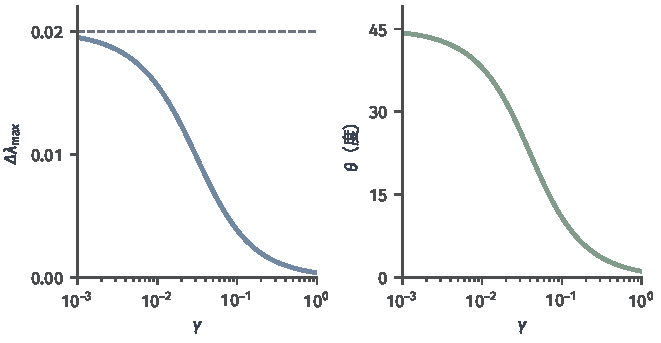
\includegraphics[width=0.92\linewidth]{figures/00-shared/mathematical-preliminaries-upper/02-linear-spaces/matplotlib/matrix-analysis-gap-direction/figure.pdf}
 \caption{谱隙与特征方向的转角（示例~\ref{ex:ls-gap-direction-rotation}，$t=0.02$）。横轴为原谱隙，
 图中记为$\gamma$，即正文的$\delta$。左：最大特征值的增量$r-\delta/2$，始终不超过虚线所示的$t$，
 符合Weyl界；右：最大特征方向的转角$\theta=\tfrac12\arctan(2t/\delta)$。谱隙远大于$t$时转角很小，
 谱隙小于$t$时转角接近$45^\circ$。}
 \label{fig:matrix-analysis-gap-direction}
\end{figure}

\paragraph{重根、奇异子空间与低秩近似}

谱隙只需存在于目标特征值组与组外之间，组内的特征值不必彼此分开。取$\bm S=\operatorname{diag}(2,2,0)$与$k=2$，原谱隙$\delta=2-0=2$。由上面的推论，$\lVert\bm E\rVert_2\leq\varepsilon<1$时，前二维特征子空间的最大主夹角满足$\sin\theta_{\max}\leq\varepsilon/(2-\varepsilon)<\varepsilon$，这个平面是稳定的。

但平面内单个特征向量的选择并不稳定：取$\eta>0$，扰动$\eta\bm e_1\bm e_1^\top$使最大特征方向成为$\bm e_1$，扰动$\eta\bm e_2\bm e_2^\top$使它成为$\bm e_2$。无论$\eta$多小，两个结果都相互正交，而前二维子空间始终是$\operatorname{span}\{\bm e_1,\bm e_2\}$。所以不能把子空间内部基的变化解释为整个子空间发生了同样大的变化，反过来，子空间稳定也不保证其中每个基向量稳定。

奇异子空间可以通过对称增广矩阵回到特征子空间。设$\bm A,\bm E\in\mathbb R^{m\times n}$，$p=\min(m,n)$，$1\leq k<p$，前$k$个左、右奇异向量排成$\bm U_k$、$\bm V_k$。要求截断处的奇异值间隙$\delta_\sigma=\sigma_k(\bm A)-\sigma_{k+1}(\bm A)>0$，这也保证了所追踪的奇异值$\sigma_1,\ldots,\sigma_k$都为正。若$\sigma_k=0$，引理~\ref{lem:ls-symmetric-augmentation-spectrum}中的$\bm w_k^+$与$\bm w_k^-$对应同一个特征值$0$，就无法从增广矩阵的特征子空间中分出相应的奇异方向。

由该引理，$\bm H(\bm A)$前$k$个特征值为$\sigma_1,\ldots,\sigma_k$，第$k+1$个为$\sigma_{k+1}$，对应的特征子空间由$\bm w_i^+$（$i\leq k$）张成，其正交投影为
\[
 \bm P_{\bm H}=\frac12\begin{bmatrix}\bm U_k\bm U_k^\top&\bm U_k\bm V_k^\top\\\bm V_k\bm U_k^\top&\bm V_k\bm V_k^\top\end{bmatrix}.
\]
现在设$\lVert\bm E\rVert_2\leq\varepsilon<\delta_\sigma/2$。由定理~\ref{thm:ls-weyl-singular-value}，$\bm A+\bm E$在截断处同样分开，对应的投影$\widetilde{\bm P}_{\bm H}$有相同的分块形式。$\bm H(\bm E)$的谱范数等于$\lVert\bm E\rVert_2$，对增广矩阵使用上面的推论，得$\lVert\bm P_{\bm H}-\widetilde{\bm P}_{\bm H}\rVert_2\leq\varepsilon/(\delta_\sigma-\varepsilon)$。矩阵左上块的谱范数不超过整个矩阵的谱范数（对单位向量$\bm x$，左上块乘$\bm x$是整个矩阵乘$(\bm x;\bm0)$所得向量的上半部分），而$\bm P_{\bm H}-\widetilde{\bm P}_{\bm H}$的左上块是$\tfrac12(\bm U_k\bm U_k^\top-\widetilde{\bm U}_k\widetilde{\bm U}_k^\top)$，所以
\[
 \lVert\bm U_k\bm U_k^\top-\widetilde{\bm U}_k\widetilde{\bm U}_k^\top\rVert_2\leq\frac{2\varepsilon}{\delta_\sigma-\varepsilon}\leq\frac{4\varepsilon}{\delta_\sigma},
\]
右下块给出右奇异子空间的同样结论。可见左、右奇异子空间的稳定性由截断处的间隙$\delta_\sigma$控制。

与上一小节对照：最佳秩$k$逼近的误差$\sigma_{k+1}$在任何情况下都只移动不超过$\varepsilon$，而取得这个误差所用的主方向只在截断处有足够间隙时才稳定。$\sigma_k=\sigma_{k+1}$时，最优误差仍然稳定，最优的秩$k$矩阵却可能在不同的子空间之间跳变。第~\ref{sec:ls-truncated-svd-ridge}节的截断求解直接用到这个区别：选取截断位置时，既要看被舍弃的奇异值是否可以忽略，也要看保留的方向是否与舍弃的方向分得开。

\subsection{一般方阵的谱敏感性}
\label{sec:ls-nonnormal-spectral-sensitivity}

前面按序比较特征值的界依靠对称结构：特征值是实数，可以排序，并能由二次型在特征子空间上的取值刻画。一般方阵的特征值可能是复数，没有自然的次序，二次型也不再与特征值对应。下面对可对角化的方阵研究另一个问题：$\bm A+\bm E$的某个特征值离$\bm A$的谱有多远。这里允许在复数域中选取特征基，向量使用复欧氏范数$\lVert\bm z\rVert_2=(\sum_i|z_i|^2)^{1/2}$，矩阵使用相应的诱导范数。

\begin{theorem}[Bauer--Fike]
\label{thm:ls-bauer-fike}
设$\bm A\in\mathbb C^{n\times n}$可对角化，$\bm A=\bm V\bm\Lambda\bm V^{-1}$，其中$\bm\Lambda=\operatorname{diag}(\lambda_1,\ldots,\lambda_n)$，$\bm V$可逆；记$\kappa_2(\bm V)=\lVert\bm V\rVert_2\lVert\bm V^{-1}\rVert_2$。则对任意$\bm E\in\mathbb C^{n\times n}$与$\bm A+\bm E$的任一特征值$\mu$，
\[
 \min_{1\leq i\leq n}|\mu-\lambda_i|\leq\kappa_2(\bm V)\lVert\bm E\rVert_2 .
\]
\end{theorem}
\begin{proof}
若$\mu$是$\bm A$的特征值，左端为零，结论成立。下设$\mu$不是$\bm A$的特征值，于是对角矩阵$\bm\Lambda-\mu\bm I$可逆。取$\bm A+\bm E$对应于$\mu$的特征向量$\bm w\neq\bm0$，由$(\bm A+\bm E)\bm w=\mu\bm w$得$(\bm A-\mu\bm I)\bm w=-\bm E\bm w$。代入$\bm A-\mu\bm I=\bm V(\bm\Lambda-\mu\bm I)\bm V^{-1}$，令$\bm y=\bm V^{-1}\bm w\neq\bm0$，得
\[
 \bm y=-(\bm\Lambda-\mu\bm I)^{-1}\bm V^{-1}\bm E\bm V\bm y .
\]
两边取范数，
\[
 \begin{aligned}
 \lVert\bm y\rVert_2
 &\leq\lVert(\bm\Lambda-\mu\bm I)^{-1}\rVert_2\,\lVert\bm V^{-1}\bm E\bm V\rVert_2\,\lVert\bm y\rVert_2\\
 &\leq\lVert(\bm\Lambda-\mu\bm I)^{-1}\rVert_2\,\kappa_2(\bm V)\lVert\bm E\rVert_2\,\lVert\bm y\rVert_2 .
 \end{aligned}
\]
对角矩阵$\bm D=\operatorname{diag}(d_i)$满足$\lVert\bm D\bm z\rVert_2^2=\sum_i|d_i|^2|z_i|^2\leq\max_i|d_i|^2\lVert\bm z\rVert_2^2$，且在相应的坐标向量处取等号，所以$\lVert(\bm\Lambda-\mu\bm I)^{-1}\rVert_2=1/\min_i|\lambda_i-\mu|$。代入并除以$\lVert\bm y\rVert_2>0$，得$1\leq\kappa_2(\bm V)\lVert\bm E\rVert_2/\min_i|\lambda_i-\mu|$，整理即得结论。
\end{proof}
界中出现的是所选特征基的条件数$\kappa_2(\bm V)$，而不是上一节的$\kappa_2(\bm A)$，二者衡量不同的东西。$\bm A=\operatorname{diag}(1,s)$（$0<s<1$）可取$\bm V=\bm I$，$\kappa_2(\bm V)=1$，任何扰动都只能使特征值移动不超过$\lVert\bm E\rVert_2$，而$\kappa_2(\bm A)=1/s$可以很大。

反过来，求逆不敏感的矩阵也可能有敏感的特征值。取$\eta>0$与
\[
 \bm A=\begin{bmatrix}1&1\\0&1+\eta\end{bmatrix},\qquad
 \bm V=\begin{bmatrix}1&1\\0&\eta\end{bmatrix},
\]
由$\bm A(1,0)^\top=(1,0)^\top$与$\bm A(1,\eta)^\top=(1+\eta)(1,\eta)^\top$，$\bm V$的两列是特征值$1$与$1+\eta$的特征向量。$\eta\to0$时，$\bm A$趋于$\bm A_0=\left[\begin{smallmatrix}1&1\\0&1\end{smallmatrix}\right]$：$\bm A_0^\top\bm A_0=\left[\begin{smallmatrix}1&1\\1&2\end{smallmatrix}\right]$的特征值为$(3\pm\sqrt5)/2$，乘积为$1$，所以$\kappa_2(\bm A_0)=\sqrt{(3+\sqrt5)/(3-\sqrt5)}=(3+\sqrt5)/2\approx2.62$；又$\lVert\bm A-\bm A_0\rVert_2=\eta$，由定理~\ref{thm:ls-weyl-singular-value}，$\bm A$的两个奇异值与$\bm A_0$的相差不超过$\eta$，$\kappa_2(\bm A)$随之趋于$\kappa_2(\bm A_0)$，求逆并不敏感。

但两个特征向量越来越接近平行：$\det(\bm V^\top\bm V)=(\det\bm V)^2$，所以$\bm V$的两个奇异值之积为$|\det\bm V|=\eta$，而最大奇异值不小于$\lVert\bm V\bm e_1\rVert_2=1$，故$\kappa_2(\bm V)\geq1/\eta$，Bauer--Fike界变得很宽。非正交的特征基会放大扰动在特征坐标中的表示，这是一般方阵特征值敏感的来源；对称矩阵可取正交的$\bm V$，$\kappa_2(\bm V)=1$，界与Weyl界同量级。

使用这个界时还要注意三点。第一，特征向量的缩放会改变$\bm V$的条件数，界对任意一组特征基成立，引用时须说明所用的基，通常取使$\kappa_2(\bm V)$较小的一组。第二，它只保证每个扰动后的特征值接近某个原特征值，不建立逐个特征值的固定配对，也不恢复对称情形的有序比较。第三，它要求$\bm A$可对角化；特征向量不足时，特征值的变化可以与扰动不成比例。
\begin{example}[特征值的移动远大于扰动]
\label{ex:ls-jordan-eigenvalue-sensitivity}
取不可对角化的
\[
 \bm A=\begin{bmatrix}0&1\\0&0\end{bmatrix},
\]
它的特征值全为$0$，特征空间只有一维。在左下角放一个大小为$t$的扰动$\bm E=\left[\begin{smallmatrix}0&0\\t&0\end{smallmatrix}\right]$，$t>0$，则$\lVert\bm E\rVert_2=t$，而
\[
 \bm A+\bm E=\begin{bmatrix}0&1\\t&0\end{bmatrix},\qquad
 \det\bigl(z\bm I-(\bm A+\bm E)\bigr)=z^2-t ,
\]
特征值为$\pm\sqrt t$，移动量为$\sqrt t$。扰动越小，这个比例反而越悬殊：$t=10^{-10}$时特征值移动$10^{-5}$，是扰动大小的$10^5$倍。由于$\sqrt t/t\to\infty$（$t\to0^+$），不存在常数$c$使移动量对所有小扰动都不超过$c\lVert\bm E\rVert_2$，Bauer--Fike那样与扰动成比例的界在这里不可能成立。若改取$t<0$，特征值为$\pm\mathrm i\sqrt{|t|}$，实特征值随之消失。
\end{example}
这个例子说明，缺少可对角化条件时，特征值的变化可以出现与扰动不同的量级；本节不为此引入新的标准形体系。第~\ref{sec:multivariable-eigenvalue-differential}节在相应光滑分支存在时研究一阶响应；本节的有限变化界则始终要连同对象的结构（对称、可对角化）和谱的分离条件一起使用。

综合起来，把矩阵本身当作输入时：对称矩阵的特征值与任意矩阵的奇异值都随扰动有界地移动，移动量不超过$\lVert\bm E\rVert_2$，并且不要求谱值分开，由此可以可靠地判断符号、正定性和秩的下界；所选子空间的方向要用主夹角比较，偏转由扰动与谱隙之比控制；一般方阵的特征值还取决于特征基的条件，甚至不与扰动成比例。条件数与谱的扰动讨论的都是一次作用或一次分解；同一个矩阵的反复作用留给第~\ref{chap:linear-recurrence-stability}章。

\FloatBarrier
\section{本章小结}
\label{sec:condition-perturbation-summary}

本章开头问：只知道误差大小的上限时，由手中的数据算出的结论还有多可靠？答案要先分清误差在哪里，再分清关心的是哪一种输出。

误差在输入向量上、矩阵固定时，线性性给出对任意大小扰动都成立的精确增量$\bm A\bm h$。绝对误差最多放大$\sigma_{\max}(\bm A)$倍，沿最大右奇异方向达到。相对误差的放大还取决于基点：固定输入处的相对条件数是$\lVert\bm A\rVert_2\lVert\bm x\rVert_2/\lVert\bm A\bm x\rVert_2$，输入落在被压缩的方向上时它大；对输入也取最坏值，得到矩阵条件数$\kappa_2(\bm A)=\sigma_{\max}/\sigma_{\min}$，它衡量最强与最弱作用之差，不衡量矩阵元素的大小，也不描述反复作用的长期趋势。

误差在矩阵本身上时，不同输出有不同的稳定性条件。对称矩阵按序配对的特征值与任意矩阵的奇异值都移动不超过$\lVert\bm E\rVert_2$，不要求谱值彼此分开；据此，区间不含零的特征值保持符号，$\lambda_{\min}(\bm S)>\varepsilon$保证正定，$\sigma_k(\bm A)>\varepsilon$保证秩至少为$k$。可逆矩阵到奇异矩阵的谱范数距离恰为$\sigma_{\min}$，相对距离为$1/\kappa_2(\bm A)$。精确秩会在任意小的扰动下跳变，可靠的只是给定误差预算下的有效秩。

所选的特征子空间要用主夹角或投影之差比较，单个特征向量的变化不能代表子空间的变化。偏转由扰动与谱隙之比控制：交叉间隔$\gamma>0$时$\sin\theta_{\max}\leq\lVert\bm E\rVert_2/\gamma$，已知原谱隙$\delta$且$\varepsilon<\delta/2$时不超过$2\varepsilon/\delta$。重特征值内部的基不稳定，但只要目标组与其余谱分开，整个子空间稳定；奇异子空间由截断处的奇异值间隙控制。

一般方阵没有对称结构。可对角化时，Bauer--Fike界使扰动后的特征值离原谱不超过$\kappa_2(\bm V)\lVert\bm E\rVert_2$，敏感性由特征基的条件数而不是$\kappa_2(\bm A)$决定；不可对角化时，特征值的移动可以与扰动不成比例，例如$\sqrt t$对$t$。

所以判断一个谱或分解的结果是否可靠，要同时说明对象的结构（对称、可对角化）、所用的分离条件（谱隙、奇异值间隙）和误差预算；仅凭$\kappa_2(\bm A)$不能判断特征值或子空间是否敏感。这些界都是有限变化界，沿指定方向的一阶响应与带余项的近似误差在第~\ref{chap:differential-perturbation-analysis}章讨论。下一章转向同一个矩阵的反复作用：误差每一步都要再经过一次作用，长期结果由谱半径决定。


% 第8章：线性递推的收敛与稳定性（递推解的表示、初值影响的衰减、固定输入下的平衡与收敛、收敛速度与短期放大、误差传播与累积）。

\chapter{线性递推的收敛与稳定性}
\label{sec:ls-convergence}
\label{sec:linear-algebra-convergence-approximation}
\label{chap:linear-recurrence-stability}

第~\ref{chap:condition-and-spectral-perturbation}章研究的是一次作用：输入或矩阵有误差时，结果能变化多少。许多计算却反复执行同一个更新：给定实方阵$\bm T\in\mathbb R^{d\times d}$与向量$\bm c\in\mathbb R^d$，从初值$\bm x_0$出发，令
\begin{equation}
 \bm x_{k+1}=\bm T\bm x_k+\bm c,\qquad k=0,1,2,\ldots
 \label{eq:ls-affine-iteration}
\end{equation}
每一轮先对当前状态作同一个线性变换，再加入同一个输入。本章要回答的问题是：无论从哪里出发，这些状态能否趋于同一个平衡？如果能，平衡在哪里，接近得多快？每一轮计算若带有小误差，误差会累积到多大？

第~\ref{sec:ls-affine-iteration-unrolling}节展开递推，把状态拆成“初值经过$k$次作用后的剩余影响”与“历次输入的累积”两部分：前者由矩阵幂$\bm T^k$描述，后者由矩阵级数$\sum_j\bm T^j$描述。第~\ref{sec:ls-matrix-power-behavior}节证明初值影响全部消失当且仅当谱半径$\rho(\bm T)<1$，这比每一步都收缩的范数条件更一般。第~\ref{sec:ls-matrix-series-exponential}节在同一条件下用Neumann级数求出输入的累积与共同的极限。第~\ref{sec:ls-convergence-rate-transient}节估计接近平衡的速度，并说明非正规矩阵可能先放大、再衰减。第~\ref{sec:ls-accumulated-step-errors}节把每一步的附加误差当作新的输入，比较有界、趋零和可求和的误差对最终精度的影响。

本章用到第~\ref{chap:eigen-spectral-decomposition}章的特征值、实Schur形、谱半径与正规矩阵，以及第~\ref{chap:singular-value-decomposition}章的谱范数。本章只分析给定的$\bm T$与$\bm c$；如何从线性方程出发构造计算便宜且能收敛的更新规则，留给第~\ref{chap:stationary-iterations}章。

本章的收敛按第~\ref{sec:ls-finite-dimensional-sequences}节理解：向量列或矩阵列收敛，等价于每个坐标或每个元素组成的实数列收敛（定理~\ref{thm:multivariable-coordinatewise-convergence}）；由有限维范数等价（定理~\ref{thm:ls-norm-equivalence}），收敛与否不随所选范数改变。所以下面主要在二范数下估计，$\lVert\bm T^k\rVert_2\to0$就是$\bm T^k\to\bm0$。矩阵级数按第~\ref{sec:ls-vector-matrix-series}节的部分和定义收敛，并使用那里的绝对收敛判据。

\section{递推解的表示}
\label{sec:ls-affine-iteration-unrolling}

先用一个二维例子看更新规则怎样逐步推进。本章始终用它说明各个结论。
\begin{example}[贯穿本章的更新]
\label{ex:ls-affine-running-example}
取下面的更新矩阵与输入：
\[
 \bm T=\begin{bmatrix}1/2&1\\0&1/2\end{bmatrix},\qquad
 \bm c=\begin{bmatrix}0\\1\end{bmatrix}.
\]
写成分量，更新是
\[
 x_{k+1,1}=\tfrac12x_{k,1}+x_{k,2},\qquad
 x_{k+1,2}=\tfrac12x_{k,2}+1 :
\]
两个分量每轮各保留一半，第二个分量还把当前值传给第一个分量，随后第二个分量补入$1$。

从$\bm x_0=\bm0$出发逐步计算，前三步是
\[
 \bm x_1=\begin{bmatrix}0\\1\end{bmatrix},\quad
 \bm x_2=\begin{bmatrix}1\\3/2\end{bmatrix},\quad
 \bm x_3=\begin{bmatrix}2\\7/4\end{bmatrix}.
\]
每一步都只是把上一步代入更新规则，例如
\[
 \bm x_3=\bm T\bm x_2+\bm c=\begin{bmatrix}\tfrac12+\tfrac32\\\tfrac34\end{bmatrix}+\begin{bmatrix}0\\1\end{bmatrix}.
\]
\end{example}
三步之后，第二个分量的增量依次为$1/2$、$1/4$，似乎在接近$2$；第一个分量每步增加$1$，看不出是否有界。换一个初值，结果是否相同，也不能由这几步判断。要回答这些问题，先把$\bm x_k$直接写成初值与输入的表达式。

\begin{lemma}[递推的有限展开]
\label{lem:ls-affine-unrolling}
对任意初值$\bm x_0$与$k\geq0$，
\begin{equation}
 \bm x_k=\bm T^k\bm x_0+\sum_{j=0}^{k-1}\bm T^j\bm c ,
 \label{eq:ls-affine-unrolling}
\end{equation}
其中$k=0$时和式为空，取为$\bm0$。
\end{lemma}
\begin{proof}
对$k$归纳。$k=0$时两边都是$\bm x_0$。设结论对$k$成立，代入更新规则，
\[
\begin{aligned}
 \bm x_{k+1}&=\bm T\Bigl(\bm T^k\bm x_0+\sum_{j=0}^{k-1}\bm T^j\bm c\Bigr)+\bm c\\
 &=\bm T^{k+1}\bm x_0+\sum_{j=1}^{k}\bm T^j\bm c+\bm T^0\bm c ,
\end{aligned}
\]
这里用了矩阵乘法对加法的分配律，并把和式的指标平移一位。末两项合起来是$\sum_{j=0}^{k}\bm T^j\bm c$，结论对$k+1$成立。
\end{proof}
展开式的第一项$\bm T^k\bm x_0$记录最初状态经过$k$轮作用后的剩余影响。和式中的$\bm T^j\bm c$是$j$轮之前加入的输入再经过$j$次作用的结果，和式把各轮输入的贡献加在一起。$\bm c=\bm0$时，只剩下反复施加同一矩阵的轨迹$\bm T^k\bm x_0$。这里只作了有限展开，还没有假定极限或平衡存在。

比较相同$\bm T,\bm c$而初值不同的两条轨迹$\bm x_k$与$\widetilde{\bm x}_k$。两者的展开式中输入部分相同，相减后只剩
\[
 \bm x_k-\widetilde{\bm x}_k=\bm T^k(\bm x_0-\widetilde{\bm x}_0).
\]
所以“初值是否影响最终结果”只取决于矩阵幂对初始差的作用。只看某一个初始差并不够，下面把“所有初始差都消失”写成关于$\bm T^k$本身的条件。

\begin{lemma}[初值差异消失的条件]
\label{lem:ls-affine-difference-decay}
对固定的$\bm T$与$\bm c$，以下两条等价：
\begin{enumerate}
 \item 对任意两个初值$\bm x_0,\widetilde{\bm x}_0$，相应轨迹满足$\bm x_k-\widetilde{\bm x}_k\to\bm0$；
 \item $\bm T^k\to\bm0$。
\end{enumerate}
\end{lemma}
\begin{proof}
由上式，第一条等价于：对任意$\bm v\in\mathbb R^d$都有$\bm T^k\bm v\to\bm0$。

设$\bm T^k\to\bm0$。按定义$\lVert\bm T^k\rVert_{\mathrm F}\to0$，而二范数不超过Frobenius范数，故对任意$\bm v$，
\[
\begin{aligned}
 \lVert\bm T^k\bm v\rVert_2&\leq\lVert\bm T^k\rVert_2\lVert\bm v\rVert_2\\
 &\leq\lVert\bm T^k\rVert_{\mathrm F}\lVert\bm v\rVert_2\to0 .
\end{aligned}
\]

反过来，设对任意$\bm v$都有$\bm T^k\bm v\to\bm0$。依次取$\bm v=\bm e_1,\ldots,\bm e_d$，$\bm T^k\bm e_j$是$\bm T^k$的第$j$列，所以每一列都趋于零。由定理~\ref{thm:multivariable-coordinatewise-convergence}，每列的各个元素趋于零，于是$\bm T^k$的每个元素趋于零，再由同一定理得$\bm T^k\to\bm0$。
\end{proof}
因此，要判断初值的影响能否全部消失，先研究矩阵幂$\bm T^k$何时趋于零；之后再回到展开式中的输入累积，寻找共同的极限。

\section{初值影响的衰减}
\label{sec:ls-matrix-power-behavior}
\label{sec:linear-algebra-power-convergence}

一个便于检验的充分条件来自范数。若某个次乘性矩阵范数满足$\lVert\bm T\rVert<1$，则$\lVert\bm T^k\rVert\leq\lVert\bm T\rVert^k\to0$，由范数等价即$\bm T^k\to\bm0$。在诱导范数下，这表示每一轮作用都把任何差异缩短到原来的$\lVert\bm T\rVert$倍以内。

贯穿例说明这个条件不必要。$\bm T(0,1)^\top=(1,1/2)^\top$，长度为$\sqrt5/2>1$，所以$\lVert\bm T\rVert_2>1$；由第~\ref{sec:ls-matrix-norms}节的列和与行和公式，$\lVert\bm T\rVert_1=\lVert\bm T\rVert_\infty=3/2$，也都大于$1$。

可是示例~\ref{ex:ls-matrix-geometric-series}已经由归纳算出
\[
 \bm T^k=2^{-k}\begin{bmatrix}1&2k\\0&1\end{bmatrix},
\]
由$k2^{-k}\to0$，各元素都趋于零，$\bm T^k\to\bm0$。$\bm T$是上三角矩阵，特征值为对角元$1/2$，谱半径$\rho(\bm T)=1/2$。

这个$\bm T$不正规：$\bm T^\top\bm T$的$(1,1)$元为$1/4$，$\bm T\bm T^\top$的$(1,1)$元为$1/4+1=5/4$。对角线上方的耦合使单步放大倍数超过$1$；第~\ref{sec:ls-general-square-spectrum}节已经指出，非正规矩阵的范数可以远大于谱半径。所以需要一个能覆盖非正规矩阵、只依赖谱半径的判据。

下面的引理是这个判据的核心。它先用相似变换把实Schur形的每个对角块化为模长乘旋转，再用逐块的坐标缩放把对角线上方的块压小，构造一个使$\bm T$的诱导范数不超过$r$的坐标范数，从而得到以略大于谱半径的$r$为底的几何上界。为了不与更新矩阵混淆，下面把$\bm T$的实Schur形（定理~\ref{thm:ls-real-schur}）记为$\bm U$。

\begin{lemma}[矩阵幂的几何上界]
\label{lem:ls-power-geometric-bound}
对任意$r>\rho(\bm T)$，存在可逆矩阵$\bm M$，使$\bm T$在坐标范数$\lVert\bm x\rVert_*=\lVert\bm M^{-1}\bm x\rVert_2$诱导的矩阵范数下满足$\lVert\bm T\rVert_*\leq r$；从而存在常数$C_r$，使$\lVert\bm T^k\rVert_2\leq C_rr^k$对所有$k\geq0$成立。
\end{lemma}
\begin{proof}
取实Schur形$\bm T=\bm Q\bm U\bm Q^\top$，其中$\bm Q$正交，$\bm U$分块上三角。设$\bm U$有$s$个对角块，第$i$块的特征值模长为$|\lambda_i|$。

先处理对角块。每个$2\times2$对角块$\bm U_{i,i}$有一对共轭特征值，按第~\ref{sec:ls-general-square-spectrum}节的论证，在复特征向量的实部、虚部组成的基下，它化为模长乘旋转：
\[
 \bm U_{i,i}=\bm P_i(|\lambda_i|\bm R_i)\bm P_i^{-1},
\]
其中$\bm R_i$为旋转矩阵；$1\times1$块取$\bm P_i=1$、$\bm R_i=\pm1$。

再压小非对角块。对$0<\varepsilon\leq1$，令分块对角矩阵
\[
 \bm D_\varepsilon=\operatorname{diag}(\varepsilon^{0}\bm P_1,\varepsilon^{1}\bm P_2,\ldots,\varepsilon^{s-1}\bm P_s).
\]
直接相乘，$\bm D_\varepsilon^{-1}\bm U\bm D_\varepsilon$的第$(i,j)$块为
\[
 \bigl(\bm D_\varepsilon^{-1}\bm U\bm D_\varepsilon\bigr)_{i,j}=\varepsilon^{j-i}\bm P_i^{-1}\bm U_{i,j}\bm P_j .
\]
对角块是$|\lambda_i|\bm R_i$。$j>i$的块带有因子$\varepsilon^{j-i}\leq\varepsilon$，所以全部非对角块组成的矩阵，其Frobenius范数不超过$\varepsilon c$，其中$c$是由各块$\bm P_i^{-1}\bm U_{i,j}\bm P_j$（$j>i$）组成的矩阵的Frobenius范数，与$\varepsilon$无关。

把矩阵拆成分块对角部分与非对角部分，得
\[
 \lVert\bm D_\varepsilon^{-1}\bm U\bm D_\varepsilon\rVert_2\leq\rho(\bm T)+\varepsilon c .
\]
这里分块对角部分的二范数不超过$\rho(\bm T)$，是因为把输入按块写成$\bm x=(\bm x_1,\ldots,\bm x_s)$后，旋转保持长度，输出的平方长度满足
\[
 \sum_i|\lambda_i|^2\lVert\bm R_i\bm x_i\rVert_2^2\leq\rho(\bm T)^2\lVert\bm x\rVert_2^2 ;
\]
非对角部分则用二范数不超过Frobenius范数估计。取$\varepsilon$足够小，使右端不超过$r$。

最后构造坐标范数并换回原坐标。令$\bm M=\bm Q\bm D_\varepsilon$，则$\bm M^{-1}\bm T\bm M=\bm D_\varepsilon^{-1}\bm U\bm D_\varepsilon$。$\bm M$可逆，$\lVert\bm x\rVert_*=\lVert\bm M^{-1}\bm x\rVert_2$是一个向量范数：齐次性与三角不等式由$\bm x\mapsto\bm M^{-1}\bm x$的线性和欧氏范数的相应性质得到，而$\lVert\bm x\rVert_*=0$意味着$\bm M^{-1}\bm x=\bm0$，由$\bm M^{-1}$可逆得$\bm x=\bm0$。它就是在新坐标$\bm M^{-1}\bm x$下量取的欧氏长度。

令$\bm x=\bm M\bm y$，它诱导的矩阵范数为
\[
\begin{aligned}
 \lVert\bm B\rVert_*
 &=\sup_{\bm x\neq\bm0}\frac{\lVert\bm M^{-1}\bm B\bm x\rVert_2}{\lVert\bm M^{-1}\bm x\rVert_2}\\
 &=\sup_{\bm y\neq\bm0}\frac{\lVert\bm M^{-1}\bm B\bm M\bm y\rVert_2}{\lVert\bm y\rVert_2}
 =\lVert\bm M^{-1}\bm B\bm M\rVert_2 .
\end{aligned}
\]
取$\bm B=\bm T$，得
\[
 \lVert\bm T\rVert_*=\lVert\bm D_\varepsilon^{-1}\bm U\bm D_\varepsilon\rVert_2\leq r .
\]
诱导范数满足次乘性，故$\lVert\bm T^k\rVert_*\leq r^k$。

再由$\bm T^k=\bm M(\bm M^{-1}\bm T^k\bm M)\bm M^{-1}$及二范数的次乘性，
\[
 \begin{aligned}
 \lVert\bm T^k\rVert_2&\leq\lVert\bm M\rVert_2\lVert\bm M^{-1}\bm T^k\bm M\rVert_2\lVert\bm M^{-1}\rVert_2\\
 &=\lVert\bm M\rVert_2\lVert\bm M^{-1}\rVert_2\lVert\bm T^k\rVert_*\\
 &\leq\lVert\bm M\rVert_2\lVert\bm M^{-1}\rVert_2\,r^k ,
 \end{aligned}
\]
取$C_r=\lVert\bm M\rVert_2\lVert\bm M^{-1}\rVert_2$即可。
\end{proof}
常数$C_r$只依赖固定的换基矩阵$\bm M$，与$k$无关；但$\bm M$随$r$选取，常数也随$r$改变。几何上界也不表示原范数下每一步都收缩：只有在坐标范数$\lVert\cdot\rVert_*$中，$\bm T$的每次作用才不超过$r$倍；换回二范数，单步放大倍数$\lVert\bm T\rVert_2$仍可能大于$1$。下面在贯穿例中具体走一遍这个构造。

\begin{example}[贯穿例的坐标范数]
\label{ex:ls-coordinate-norm-contraction}
贯穿例的$\bm T$已经是上三角矩阵，构造中的前两步都不必做：可取$\bm Q=\bm I$，两个$1\times1$对角块的$\bm P_i=1$，于是$\bm M=\bm D_\varepsilon=\operatorname{diag}(1,\varepsilon)$，且
\[
 \bm M^{-1}\bm T\bm M=\begin{bmatrix}1/2&\varepsilon\\0&1/2\end{bmatrix}.
\]
缩放把右上角的耦合从$1$压到$\varepsilon$，对角元不变。

取$\varepsilon=1/4$，剩下的任务是算出这个矩阵的二范数。为此对$a,b>0$考虑一般的矩阵及其Gram矩阵：
\[
 \bm G=\begin{bmatrix}a&b\\0&a\end{bmatrix},\qquad
 \bm G^\top\bm G=\begin{bmatrix}a^2&ab\\ab&a^2+b^2\end{bmatrix}.
\]
由式~\eqref{eq:matrix-analysis-spectral-norm}，$\lVert\bm G\rVert_2$是最大奇异值，其平方是$\bm G^\top\bm G$的最大特征值（第~\ref{chap:singular-value-decomposition}章）。这个矩阵的迹为$2a^2+b^2$、行列式为$a^4$，最大特征值为
\[
 \mu=\frac{2a^2+b^2+b\sqrt{b^2+4a^2}}{2}=\Bigl(\frac{b+\sqrt{b^2+4a^2}}{2}\Bigr)^2,
\]
第二个等号展开右端平方即可验证。所以
\[
 \lVert\bm G\rVert_2=\frac{b+\sqrt{b^2+4a^2}}{2}.
\]
代入$a=1/2$、$b=1/4$得
\[
 \lVert\bm T\rVert_*=\frac{1+\sqrt{17}}{8}\approx0.640,
\]
其中$\lVert\bm x\rVert_*=\lVert\bm M^{-1}\bm x\rVert_2=\sqrt{x_1^2+16x_2^2}$。这个值小于$1$，但比$\rho(\bm T)=1/2$大一些，对应引理中的$r$。

换回欧氏范数还需要常数$\lVert\bm M\rVert_2\lVert\bm M^{-1}\rVert_2$。对角矩阵$\operatorname{diag}(d_1,d_2)$满足
\[
 \lVert\operatorname{diag}(d_1,d_2)\bm x\rVert_2^2=d_1^2x_1^2+d_2^2x_2^2\leq\max_id_i^2\lVert\bm x\rVert_2^2 ,
\]
且在相应的标准基向量处取等号，故其二范数为$\max_i|d_i|$。于是$\lVert\bm M\rVert_2=1$、$\lVert\bm M^{-1}\rVert_2=\lVert\operatorname{diag}(1,4)\rVert_2=4$，所以
\[
 \lVert\bm T^k\rVert_2\leq4\times0.641^k .
\]
在加大了第二坐标权重的范数中，$\bm T$每一步都收缩；换回欧氏长度，代价是常数$4$。

能否把$\varepsilon$取得更小，直接让$r=\rho(\bm T)=1/2$？不能。由$\bm T^k$的显式式，
\[
 \lVert\bm T^k\rVert_2\geq\lVert\bm T^k\bm e_2\rVert_2\geq k2^{1-k},
\]
即$\lVert\bm T^k\rVert_2/2^{-k}\geq2k$，没有与$k$无关的常数能控制它；所以引理中的$r$必须严格大于谱半径。
\end{example}

有了几何上界，就能给出矩阵幂衰减的充要条件。
\begin{theorem}[矩阵幂的衰减判据]
\label{thm:ls-power-decay}
对实方阵$\bm T$，$\bm T^k\to\bm0$当且仅当$\rho(\bm T)<1$。
\end{theorem}
\begin{proof}
充分性：取$r$满足$\rho(\bm T)<r<1$。由引理~\ref{lem:ls-power-geometric-bound}，$\lVert\bm T^k\rVert_2\leq C_rr^k$，右端是公比小于$1$的几何数列，趋于零，所以$\bm T^k\to\bm0$。

必要性：设有特征值$|\lambda|\geq1$，要找出一个不趋于零的轨迹。若$\bm T^k\to\bm0$，则对任一固定向量$\bm v$，$\lVert\bm T^k\bm v\rVert_2\leq\lVert\bm T^k\rVert_2\lVert\bm v\rVert_2\to0$。

若$\lambda$为实数，取其特征向量$\bm v$，则
\[
 \lVert\bm T^k\bm v\rVert_2=|\lambda|^k\lVert\bm v\rVert_2\geq\lVert\bm v\rVert_2 ,
\]
不趋于零。

若$\lambda$非实，取第~\ref{sec:ls-general-square-spectrum}节中对应的二维实不变子空间的基$\bm u,\bm w$，排成列满秩矩阵$\bm P=[\bm u\;\bm w]$；按该节，$\bm T^k\bm P=\bm P|\lambda|^k\bm R^k$，$\bm R$为旋转矩阵。取$\bm P$的左逆$\bm L=(\bm P^\top\bm P)^{-1}\bm P^\top$，则
\[
 \bm L\bm T^k\bm u=|\lambda|^k\bm R^k\bm e_1 ,
\]
其长度为$|\lambda|^k$，所以
\[
 \lVert\bm T^k\bm u\rVert_2\geq\frac{|\lambda|^k}{\lVert\bm L\rVert_2}\geq\frac1{\lVert\bm L\rVert_2}>0,
\]
同样不趋于零。两种情形都有$\bm T^k\not\to\bm0$。
\end{proof}
结合引理~\ref{lem:ls-affine-difference-decay}，所有初值差异都会消失，当且仅当$\rho(\bm T)<1$。判据要求的是全体初值，下面两个例子分别说明，检查一个初始差，或只检查每条轨迹各自收敛，都不足以代替它。

\begin{example}[反例：一个初始差衰减不能说明全部衰减]
\label{ex:ls-partial-convergence}
取$\bm T=\operatorname{diag}(1/2,2)$，比较两个初始差的演化：
\[
\begin{gathered}
\bm T^k\begin{bmatrix}1\\0\end{bmatrix}=\begin{bmatrix}2^{-k}\\0\end{bmatrix}\to\bm0\\
\bm T^k\begin{bmatrix}0\\1\end{bmatrix}=\begin{bmatrix}0\\2^k\end{bmatrix},
\end{gathered}
\]
后者的长度为$2^k\to\infty$。初始差$(1,0)^\top$恰好不含增长方向$\bm e_2$的分量，所以差异消失；初始差$(0,1)^\top$则沿$\bm e_2$被不断放大。这里$\rho(\bm T)=2>1$，判据并不成立。可见只检查某个特殊的初始差，可能恰好避开了增长方向，不能据此断言$\bm T^k\to\bm0$。
\end{example}

\begin{example}[反例：各轨迹收敛但极限不同]
\label{ex:ls-separate-limits}
取$\bm T=\operatorname{diag}(1,1/2)$、$\bm c=\bm0$。对任意初值，
\[
 \bm x_k=\bm T^k\bm x_0=\begin{bmatrix}x_{0,1}\\2^{-k}x_{0,2}\end{bmatrix}\to\begin{bmatrix}x_{0,1}\\0\end{bmatrix}.
\]
每条轨迹都有极限，但极限保留了初值的第一个坐标：特征值$1$的方向上，初值既不衰减也不增长，一直被记住。所以不同初值趋于不同的点。这里$\rho(\bm T)=1$，$\bm T^k\to\operatorname{diag}(1,0)\neq\bm0$。各轨迹分别收敛，并不等于它们趋于同一极限；后者才要求$\bm T^k\to\bm0$。
\end{example}

$\rho(\bm T)=1$时，由定理~\ref{thm:ls-power-decay}，$\bm T^k\not\to\bm0$，再由引理~\ref{lem:ls-affine-difference-decay}，初值差异不会全部消失；但不同矩阵的轨迹表现不同，下面看几个例子。

仍取$\bm c=\bm0$。$\bm T=\bm I$时$\bm x_k=\bm x_0$，每条轨迹恒定，有界且收敛，但极限就是初值本身；$\bm T=-\bm I$时$\bm x_k=(-1)^k\bm x_0$，非零初值的轨迹来回翻转，有界而不收敛。

再看平面上的$90^\circ$旋转
\[
 \bm R=\begin{bmatrix}0&-1\\1&0\end{bmatrix}.
\]
它的特征值为$\pm\mathrm i$，谱半径为$1$；它保持长度，$\lVert\bm R^k\bm x_0\rVert_2=\lVert\bm x_0\rVert_2$，又$\bm R^4=\bm I$而$\bm R\bm x_0\neq\bm x_0$（$\bm x_0\neq\bm0$），所以非零初值的轨迹以$4$步为周期循环，有界而不收敛。

下例说明，特征向量不够时还会出现增长。
\begin{example}[反例：谱半径为$1$而矩阵幂无界]
\label{ex:ls-unit-spectral-radius-growth}
考虑
\[
 \bm J_1=\begin{bmatrix}1&1\\0&1\end{bmatrix}.
\]
它只有特征值$1$，$\rho(\bm J_1)=1$，特征向量却只有$(1,0)^\top$的倍数。按示例~\ref{ex:ls-jordan-block-power}的二项式展开，把$0.8$换成$1$，得
\[
 \bm J_1^k=(\bm I+\bm N)^k=\bm I+k\bm N=\begin{bmatrix}1&k\\0&1\end{bmatrix}.
\]
对角元始终是$1$，与谱半径相符；增长全在右上角，它随$k$线性变大，$\lVert\bm J_1^k\rVert_2\geq k\to\infty$。与$\bm I$、$-\bm I$和旋转相比，缺少的正是第二条特征方向。所以谱半径等于$1$不能保证矩阵幂有界。
\end{example}
这种多项式因子来自对角线上方的耦合。考虑$s$阶矩阵$\bm J=\lambda\bm I+\bm N$，其中$\bm N$是超对角元为$1$、其余元素为零的矩阵，满足$\bm N^s=\bm0$；这样的矩阵称为Jordan块，上例是$\lambda=1$、$s=2$的情形。本节只用这一具体形式，不需要一般的Jordan理论。$\lambda\bm I$与$\bm N$可交换，二项式展开成立，且$j\geq s$的项为零：
\begin{equation}
 \bm J^k=\sum_{j=0}^{\min(k,s-1)}\binom{k}{j}\lambda^{k-j}\bm N^j .
 \label{eq:ch06-jordan-power}
\end{equation}

由这个展开可以读出块幂何时有界。其中$\binom kj\leq k^j$，$j\leq s-1$。当$s\geq2$、$|\lambda|=1$时，$\bm J^k$的$(1,2)$元为$k\lambda^{k-1}$，模为$k\to\infty$，矩阵幂无界。

当$|\lambda|<1$时块幂仍趋于零。$\lambda=0$时$\bm J^k=\bm N^k$在$k\geq s$时为零。$0<|\lambda|<1$时，$\bm J^k$的非零元为$\binom kj\lambda^{k-j}$，模不超过$|\lambda|^{-j}a_k$，其中$a_k=k^j|\lambda|^k$。相邻两项之比满足
\[
 \frac{a_{k+1}}{a_k}=\Bigl(1+\frac1k\Bigr)^j|\lambda|\to|\lambda|<1 .
\]
取$q$满足$|\lambda|<q<1$，则$k$充分大后$a_{k+1}\leq qa_k$，$a_k$被一个公比为$q$的几何数列控制，趋于零。

不过多项式因子可能使块幂在衰减之前先上升。把上例的特征值从$1$降到$0.8$，就能看到这种先升后降。
\begin{example}[Jordan块幂的先升后降]
\label{ex:ls-jordan-transient}
从初值$(0,1)^{\top}$出发，反复作用下面的矩阵：
\[
 \bm J=\begin{bmatrix}0.8&1\\0&0.8\end{bmatrix}.
\]
由示例~\ref{ex:ls-jordan-block-power}，
\[
 \bm J^k\begin{bmatrix}0\\1\end{bmatrix}=\begin{bmatrix}k\,0.8^{k-1}\\0.8^k\end{bmatrix}.
\]
第二坐标按$0.8^k$单调衰减。第一坐标在$k=1,2,\ldots,6$时依次为$1$、$1.6$、$1.92$、$2.048$、$2.048$、$1.966$（末项保留三位小数），在$k=4,5$时达到最大值约$2.05$，此后才衰减。

这与示例~\ref{ex:ls-jordan-block-power}中相邻项之比$0.8(k+1)/k$在$k=4$处等于$1$相符。特征值$0.8<1$保证最终衰减，但在开始几步，多项式因子$k$的增长胜过$0.8^{k-1}$的衰减，使第一坐标先上升到初值长度的两倍以上。
\end{example}
图~\ref{fig:vol1-add-linear-jordan-accumulation}画出这条轨迹的两个坐标。

多项式因子也会抬高引理~\ref{lem:ls-power-geometric-bound}中的常数$C_r$。以贯穿例为例，任何对所有$k$满足$\lVert\bm T^k\rVert_2\leq C_rr^k$的常数，都要对每个$k$满足（示例~\ref{ex:ls-coordinate-norm-contraction}）
\[
 C_r\geq\frac{k2^{1-k}}{r^k}.
\]
固定$k$令$r\downarrow1/2$，右端趋于$2k$。所以$r$越接近$\rho(\bm T)$，可用的常数就必须越大，且没有上界。

\begin{figure}[!htb]
  \centering
  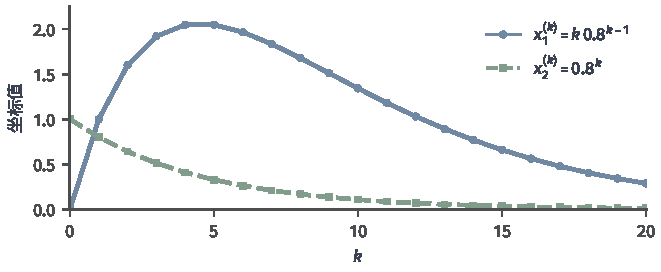
\includegraphics[width=112mm]{figures/00-shared/mathematical-preliminaries-upper/02-linear-spaces/matplotlib/comprehension-additions/linear-jordan-accumulation.pdf}
  \caption{Jordan块的累积项。取正文$\bm J=\left[\begin{smallmatrix}0.8&1\\0&0.8\end{smallmatrix}\right]$与初值$(0,1)^{\top}$。绿线为$0.8^k$，蓝线在$k\geq1$时为$k0.8^{k-1}$，在$k=0$时为$0$。点表示整数步，连线仅引导读图；两坐标最终都趋零。}
  \label{fig:vol1-add-linear-jordan-accumulation}
\end{figure}

$\rho(\bm T)>1$时，由定理~\ref{thm:ls-power-decay}必要性的证明，从模大于$1$的特征值的特征方向（或不变平面）出发的初始差不会消失；但如示例~\ref{ex:ls-partial-convergence}所示，仍可能有特殊初值的差异趋于零。

\section{固定输入下的平衡与收敛}
\label{sec:ls-matrix-series-exponential}

初值的影响由$\bm T^k$决定，现在回到展开式中的输入累积。若所有轨迹趋于同一个点$\bm x_\star$，在更新规则两边取极限（矩阵乘法是连续的线性作用），它必须满足平衡方程
\[
 \bm x_\star=\bm T\bm x_\star+\bm c ,\quad\text{即}\quad(\bm I-\bm T)\bm x_\star=\bm c .
\]
满足这个方程的点称为更新的平衡点：从它出发，更新不再改变状态。下面的定理说明平衡何时存在唯一，以及何时吸引所有初值。

\begin{theorem}[共同极限的判据]
\label{thm:ls-affine-common-limit}
对固定的$\bm T$与$\bm c$，从任意初值出发的轨迹都收敛到同一个向量，当且仅当$\rho(\bm T)<1$。此时$\bm I-\bm T$可逆，共同极限为$\bm x_\star=(\bm I-\bm T)^{-1}\bm c$，且
\begin{equation}
 \bm x_k-\bm x_\star=\bm T^k(\bm x_0-\bm x_\star).
 \label{eq:ls-affine-common-limit}
\end{equation}
\end{theorem}
\begin{proof}
设$\rho(\bm T)<1$。$1$的模不小于$1$，不是$\bm T$的特征值，所以$\det(\bm I-\bm T)\neq0$，$\bm I-\bm T$可逆，平衡方程有唯一解$\bm x_\star=(\bm I-\bm T)^{-1}\bm c$。

把$\bm x_{k+1}=\bm T\bm x_k+\bm c$与$\bm x_\star=\bm T\bm x_\star+\bm c$相减，得
\[
 \bm x_{k+1}-\bm x_\star=\bm T(\bm x_k-\bm x_\star),
\]
归纳即得所述等式。由定理~\ref{thm:ls-power-decay}，$\bm T^k\to\bm0$，再由引理~\ref{lem:ls-affine-difference-decay}的证明，$\bm T^k(\bm x_0-\bm x_\star)\to\bm0$，即每条轨迹都收敛到$\bm x_\star$。

反过来，设所有轨迹都收敛到同一个向量$\bm x$。任取两个初值，两条轨迹之差收敛到$\bm x-\bm x=\bm0$。由引理~\ref{lem:ls-affine-difference-decay}，$\bm T^k\to\bm0$，再由定理~\ref{thm:ls-power-decay}，$\rho(\bm T)<1$。
\end{proof}
单有$\bm I-\bm T$可逆，只保证平衡唯一，不保证它吸引其他初值。例如$\bm T=2\bm I$时$\bm I-\bm T=-\bm I$可逆，平衡为$\bm x_\star=-\bm c$，但
\[
 \bm x_k-\bm x_\star=2^k(\bm x_0-\bm x_\star),
\]
除非从平衡出发，轨迹都远离平衡。

定理给出了平衡的位置，但没有说明它怎样由历次输入累积而成。回到有限展开：从$\bm x_0=\bm0$出发，
\[
 \bm x_k=\sum_{j=0}^{k-1}\bm T^j\bm c ,
\]
正是矩阵级数$\sum_j\bm T^j$的部分和作用在$\bm c$上。

按第~\ref{sec:ls-vector-matrix-series}节的定义，矩阵级数$\sum_{j=0}^{\infty}\bm T^j$收敛，指部分和$\bm S_N=\sum_{j=0}^N\bm T^j$作为矩阵序列收敛。对标量$a$，$|a|<1$时几何级数$\sum_ja^j=1/(1-a)$；矩阵情形有同样的结论。

\begin{theorem}[Neumann级数与逆]
\label{thm:ls-neumann}
若$\rho(\bm T)<1$，则级数$\sum_{j=0}^{\infty}\bm T^j$绝对收敛，$\bm I-\bm T$可逆，且
\begin{equation}
 (\bm I-\bm T)^{-1}=\sum_{j=0}^{\infty}\bm T^j .
 \label{eq:ls-neumann-series}
\end{equation}
反之，若这个级数收敛，则$\bm T^k\to\bm0$，从而$\rho(\bm T)<1$。若进一步在某个次乘性矩阵范数下$\lVert\bm T\rVert\leq q<1$，则截断误差满足
\begin{equation}
 \Bigl\lVert(\bm I-\bm T)^{-1}-\sum_{j=0}^{N}\bm T^j\Bigr\rVert\leq\frac{q^{N+1}}{1-q}.
 \label{eq:ls-neumann-tail}
\end{equation}
\end{theorem}
\begin{proof}
先证绝对收敛。取$r$满足$\rho(\bm T)<r<1$，由引理~\ref{lem:ls-power-geometric-bound}，$\lVert\bm T^j\rVert_2\leq C_rr^j$。右端是收敛的标量几何级数的通项，所以$\sum_j\lVert\bm T^j\rVert_2$收敛。由定理~\ref{thm:ls-absolute-series-convergence}，级数$\sum_j\bm T^j$收敛，记其和为$\bm S$，即$\bm S_N\to\bm S$。

再识别级数的和。逐项相消得有限几何和恒等式
\[
 \bm S_N(\bm I-\bm T)=(\bm I-\bm T)\bm S_N=\bm I-\bm T^{N+1}.
\]
令$N\to\infty$。左端是部分和乘以固定矩阵$\bm I-\bm T$。乘以固定矩阵是连续的线性作用（第~\ref{sec:multivariable-continuity}节），具体地，
\[
\begin{aligned}
 &\lVert\bm S_N(\bm I-\bm T)-\bm S(\bm I-\bm T)\rVert_2\\
 &\qquad\leq\lVert\bm S_N-\bm S\rVert_2\lVert\bm I-\bm T\rVert_2\to0 ,
\end{aligned}
\]
左乘同理，所以左端分别收敛到$\bm S(\bm I-\bm T)$与$(\bm I-\bm T)\bm S$；右端由定理~\ref{thm:ls-power-decay}收敛到$\bm I$。极限唯一，故
\[
 \bm S(\bm I-\bm T)=(\bm I-\bm T)\bm S=\bm I ,
\]
即$\bm I-\bm T$可逆且$(\bm I-\bm T)^{-1}=\bm S$，这就是式~\eqref{eq:ls-neumann-series}。

反过来，若级数收敛，收敛级数的通项趋于零（第~\ref{sec:ls-vector-matrix-series}节）：$\bm T^k=\bm S_k-\bm S_{k-1}\to\bm S-\bm S=\bm0$。再由定理~\ref{thm:ls-power-decay}得$\rho(\bm T)<1$。

最后证截断界。设$\lVert\bm T\rVert\leq q<1$，由次乘性，$\lVert\bm T^j\rVert\leq q^j$，所以级数在这个范数下也绝对收敛。由定理~\ref{thm:ls-absolute-series-convergence}的尾和估计，
\[
 \Bigl\lVert(\bm I-\bm T)^{-1}-\bm S_N\Bigr\rVert
 \leq\sum_{j=N+1}^{\infty}\lVert\bm T^j\rVert
 \leq\sum_{j=N+1}^{\infty}q^j=\frac{q^{N+1}}{1-q},
\]
即式~\eqref{eq:ls-neumann-tail}。
\end{proof}
于是$\rho(\bm T)<1$时，部分和满足$\sum_{j\leq N}\bm T^j\bm c=\bm S_N\bm c$，而
\[
 \lVert\bm S_N\bm c-\bm S\bm c\rVert_2\leq\lVert\bm S_N-\bm S\rVert_2\lVert\bm c\rVert_2\to0 ,
\]
所以
\[
 \bm x_\star=(\bm I-\bm T)^{-1}\bm c=\sum_{j=0}^{\infty}\bm T^j\bm c :
\]
平衡就是全部历次输入经各自轮数传播后的总和。

矩阵级数收敛的充要条件也是$\rho(\bm T)<1$。但这一结论针对整个矩阵级数；仅有某一个$\bm c$对应的向量级数$\sum_j\bm T^j\bm c$收敛，推不出同样的结论。例如$\bm T=\operatorname{diag}(1/2,2)$、$\bm c=(1,0)^\top$时，$\sum_j\bm T^j\bm c=(2,0)^\top$收敛，而$\rho(\bm T)=2$。

\begin{example}[贯穿例的平衡]
\label{ex:ls-affine-running-equilibrium}
现在可以回答示例~\ref{ex:ls-affine-running-example}开头留下的问题。平衡方程是上三角的，从第二个分量解起：
\[
 x_{\star,2}=\tfrac12x_{\star,2}+1,\qquad\text{得}\quad x_{\star,2}=2 .
\]
再解第一个分量：
\[
 x_{\star,1}=\tfrac12x_{\star,1}+x_{\star,2},\qquad\text{得}\quad x_{\star,1}=4 .
\]

示例~\ref{ex:ls-matrix-geometric-series}已经求出$\bm I-\bm T$的逆，用它核对：
\[
 \bm x_\star=(\bm I-\bm T)^{-1}\bm c=\begin{bmatrix}2&4\\0&2\end{bmatrix}\begin{bmatrix}0\\1\end{bmatrix}=\begin{bmatrix}4\\2\end{bmatrix}.
\]

也可以按级数逐项看平衡怎样累积而成。$j$轮之前加入的输入如今是$\bm T^j\bm c=2^{-j}(2j,1)^\top$；由示例~\ref{ex:ls-matrix-geometric-series}中的两个标量级数
\[
 \sum_j2^{-j}=2,\qquad\sum_jj\,2^{1-j}=4 ,
\]
两个分量的和分别为$4$与$2$，与上式一致。

所以开头三步中第一个分量每步加$1$的增长不会无限持续，状态趋于$(4,2)^\top$；由于$\rho(\bm T)=1/2<1$，初值项$\bm T^k\bm x_0$趋于零，从任何初值出发都得到同一个平衡。
\end{example}

Neumann级数定理分开了两种条件。$\rho(\bm T)<1$是级数收敛的充要条件，但只给出定性的收敛；$\lVert\bm T\rVert\leq q<1$是便于检验的充分条件，它给出可以直接计算的截断误差上界。

设向量范数与它诱导的矩阵范数满足$\lVert\bm T\rVert\leq q<1$。从$\bm x_0=\bm0$出发，第$k$步只累积到$k-1$次幂，
\[
 \bm x_\star-\bm x_k=\bigl((\bm I-\bm T)^{-1}-\bm S_{k-1}\bigr)\bm c .
\]
由式~\eqref{eq:ls-neumann-tail}（取$N=k-1$）与诱导范数的定义，
\begin{equation}
 \lVert\bm x_k-\bm x_\star\rVert\leq\frac{q^k}{1-q}\lVert\bm c\rVert .
 \label{eq:ls-neumann-iterate-error}
\end{equation}
图~\ref{fig:ls-neumann-series-tail}用一个$2\times2$例子核对矩阵尾界。

\begin{figure}[htbp]
 \centering
 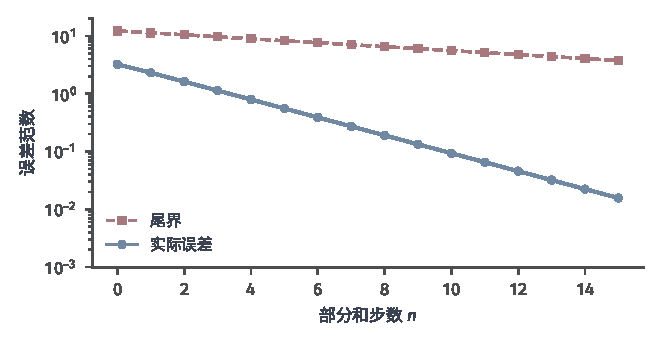
\includegraphics[width=112mm]{figures/00-shared/mathematical-preliminaries-upper/02-linear-spaces/matplotlib/ls-neumann-series-tail/ls-neumann-series-tail.pdf}
 \caption{Neumann级数尾界。$\bm T=[[0.7,0.6],[0,0.1]]$，$q=\lVert\bm T\rVert_2
 \approx0.924<1$，$(\bm I-\bm T)^{-1}=\sum\bm T^k$。蓝线为真实残差
 $\lVert\bm R_n\rVert=\lVert\bm T^{n+1}(\bm I-\bm T)^{-1}\rVert$，红虚线为尾界
 $q^{n+1}/(1-q)$，纵轴半对数（$n=0,\dots,15$）。}
 \label{fig:ls-neumann-series-tail}
\end{figure}

只知道$\rho(\bm T)<1$时，由引理~\ref{lem:ls-power-geometric-bound}，可以取$r<1$并构造坐标范数$\lVert\cdot\rVert_*$，使$\lVert\bm T\rVert_*\leq r$，于是上面的尾界在这个范数中成立。但这个范数依赖换基矩阵$\bm M$；回到原来的误差度量时，须保留比较常数。例如由$\lVert\bm B\rVert_2\leq\lVert\bm M\rVert_2\lVert\bm M^{-1}\rVert_2\lVert\bm B\rVert_*$，二范数下的尾界要再乘以$\lVert\bm M\rVert_2\lVert\bm M^{-1}\rVert_2$。

在贯穿例中，示例~\ref{ex:ls-coordinate-norm-contraction}的范数给出$q=(1+\sqrt{17})/8$与$\lVert\bm c\rVert_*=4$。又$\lVert\bm x\rVert_2\leq\sqrt{x_1^2+16x_2^2}=\lVert\bm x\rVert_*$，所以
\[
 \lVert\bm x_k-\bm x_\star\rVert_2\leq\frac{4q^k}{1-q}\approx11.1\times0.641^k .
\]
例如$k=3$时真实误差$\lVert(2,1/4)^\top\rVert_2\approx2.02$，上界约为$2.92$。

上面的结论都要求每一轮加入同一个$\bm c$。若输入随轮次变化，更新成为$\bm x_{k+1}=\bm T\bm x_k+\bm c_k$，与引理~\ref{lem:ls-affine-unrolling}相同的归纳给出
\[
 \bm x_k=\bm T^k\bm x_0+\sum_{j=0}^{k-1}\bm T^{k-1-j}\bm c_j .
\]
这时和式中的各项不再是同一个矩阵级数作用在固定向量上，平衡方程也失去意义：一般没有一个点能同时满足每一轮的更新。

$\rho(\bm T)<1$仍保证初值的影响消失，因为两条轨迹之差仍是$\bm T^k(\bm x_0-\widetilde{\bm x}_0)$；但它不保证轨迹本身收敛。例如$\bm T=\bm0$时$\bm x_k=\bm c_{k-1}$，轨迹完全复制输入；取$\bm c_k=(-1)^k\bm c$（$\bm c\neq\bm0$），轨迹来回翻转，没有极限。

所以逐步输入下轨迹的去向取决于输入序列本身。输入趋于固定值的情形，可以看作固定输入加上逐步误差，在第~\ref{sec:ls-accumulated-step-errors}节处理。

\section{收敛速度与短期放大}
\label{sec:ls-convergence-rate-transient}

谱判据回答了能否收敛，下一个问题是接近平衡有多快。设$\rho(\bm T)<1$，记误差$\bm e_k=\bm x_k-\bm x_\star$。由定理~\ref{thm:ls-affine-common-limit}，$\bm e_k=\bm T^k\bm e_0$；取$\rho(\bm T)<r<1$，由引理~\ref{lem:ls-power-geometric-bound}，
\[
 \lVert\bm e_k\rVert_2\leq C_rr^k\lVert\bm e_0\rVert_2 .
\]
误差至少按略大于谱半径的公比几何衰减。

这是对所有初始误差一致成立的上界；某些初始方向的实际误差衰减得更快。例如在贯穿例中，$\bm T\bm e_1=\tfrac12\bm e_1$，取$\bm e_0=\bm e_1$时$\bm e_k=2^{-k}\bm e_1$，每步恰好减半；而下面将看到，从$\bm e_2$出发的误差长度带有因子$2k$。

谱半径只决定接近平衡的速度，平衡的位置由$\bm c$与$(\bm I-\bm T)^{-1}$决定。

图~\ref{fig:ls-spectral-radius-convergence}显示最简单的正规情形：误差每步乘以$\rho$，$\rho<1$时衰减，$\rho>1$时增长。

\begin{figure*}[htbp]
 \centering
 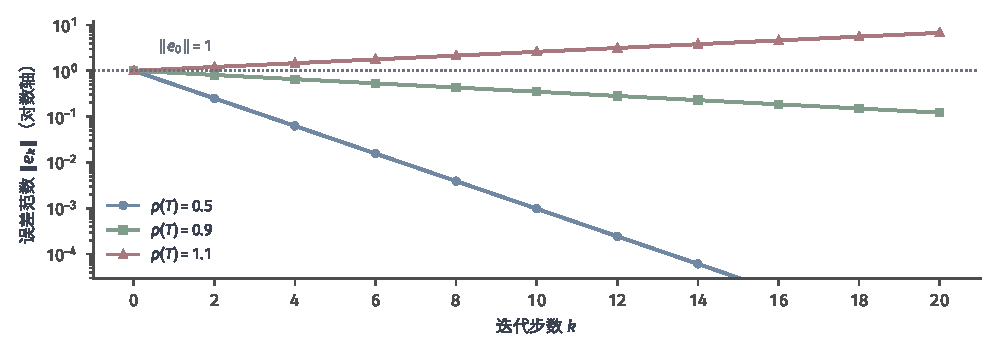
\includegraphics[width=169.0mm]{figures/00-shared/mathematical-preliminaries-upper/02-linear-spaces/matplotlib/ls-spectral-radius-convergence/ls-spectral-radius-convergence.pdf}
 \caption{谱半径决定迭代的长期方向。递推$\bm e^{(t+1)}=\bm A\bm e^{(t)}$、
 $\lVert\bm e^{(0)}\rVert=1$，取正规矩阵$\bm A=\rho\bm I$时$\lVert\bm e^{(t)}\rVert=\rho^t$：
 $\rho=0.5$（蓝）约十四步降到$10^{-4}$，$\rho=0.9$（绿）缓慢下降，
 $\rho=1.1$（红）指数上升。纵轴为半对数。}
 \label{fig:ls-spectral-radius-convergence}
\end{figure*}

上界中的常数$C_r$可能大于$1$，所以长期衰减不排除误差在前几步变大。贯穿例就是这样。
\begin{example}[贯穿例的暂时放大]
\label{ex:ls-running-transient}
在示例~\ref{ex:ls-affine-running-example}中取初值$\bm x_0=\bm x_\star+(0,1)^\top=(4,3)^\top$，即初始误差$\bm e_0=(0,1)^\top$，长度为$1$。由$\bm T^k$的显式式，
\[
 \bm e_k=\bm T^k\bm e_0=2^{-k}\begin{bmatrix}2k\\1\end{bmatrix}.
\]
前三步（$k=1,2,3$）的误差依次为
\[
 \begin{bmatrix}1\\1/2\end{bmatrix},\quad
 \begin{bmatrix}1\\1/4\end{bmatrix},\quad
 \begin{bmatrix}3/4\\1/8\end{bmatrix},
\]
长度约为$1.118$、$1.031$、$0.760$。

若误差每步按谱半径减半，前两步应为$0.5$与$0.25$；实际上前两步的误差都比初始误差还长，此后才衰减。谱半径$1/2$描述的只是长期的衰减速度。
\end{example}
放大来自方向之间的耦合：第二个分量的误差每步把自身传给第一个分量，在第二个分量衰减之前，第一个分量先积累起来。下面的例子耦合更强，放大也更明显。
\begin{example}[非正规矩阵的瞬态放大]
\label{ex:ls-transient-growth}
换一个耦合更强的更新矩阵$\bm B$，并取$\bm c=\bm0$。下面用以下更新与初值演示：
\[
\begin{gathered}
\bm B=\begin{bmatrix}0.8&4\\0&0.5\end{bmatrix}\\
\bm x_{k+1}=\bm B\bm x_k\\
\bm x_0=(0,1)^{\top}.
\end{gathered}
\]
示例~\ref{ex:ls-triangular-power}已把初值沿特征向量$\bm v_1=(1,0)^{\top}$、$\bm v_2=(-40/3,1)^{\top}$分解为
\[
 \bm x_0=\tfrac{40}{3}\bm v_1+\bm v_2 ,
\]
并写出了矩阵幂与轨迹：
\[
\begin{gathered}
\bm B^k=
 \begin{bmatrix}
  0.8^k&\frac{40}{3}(0.8^k-0.5^k)\\
  0&0.5^k
 \end{bmatrix}\\
\bm x_k=
 \begin{bmatrix}\frac{40}{3}(0.8^k-0.5^k)\\0.5^k\end{bmatrix}.
\end{gathered}
\]
代入$k=1,2,3$得
\[
 \bm x_1=\begin{bmatrix}4\\0.5\end{bmatrix},\quad
 \bm x_2=\begin{bmatrix}5.2\\0.25\end{bmatrix},\quad
 \bm x_3=\begin{bmatrix}5.16\\0.125\end{bmatrix},
\]
长度分别约为$4.03$、$5.21$、$5.16$，都远大于初值的长度$1$。

另一方面$\rho(\bm B)=0.8<1$，由定理~\ref{thm:ls-power-decay}，轨迹最终趋于零。与贯穿例只放大约$12\%$相比，这里的轨迹先放大到五倍以上、再衰减；谱半径小于$1$并不限制早期放大的幅度。
\end{example}
放大的原因在于初值沿特征方向的分解。$\tfrac{40}{3}\bm v_1=(40/3,0)^\top$与$\bm v_2=(-40/3,1)^\top$都很长、方向几乎相反，初值$(0,1)^\top$由二者相消而成。两个分量衰减速度不同，相消很快被打破，所以长度先增后降（图~\ref{fig:ch06-transient-growth}）。

\begin{figure*}[htbp]
  \centering
  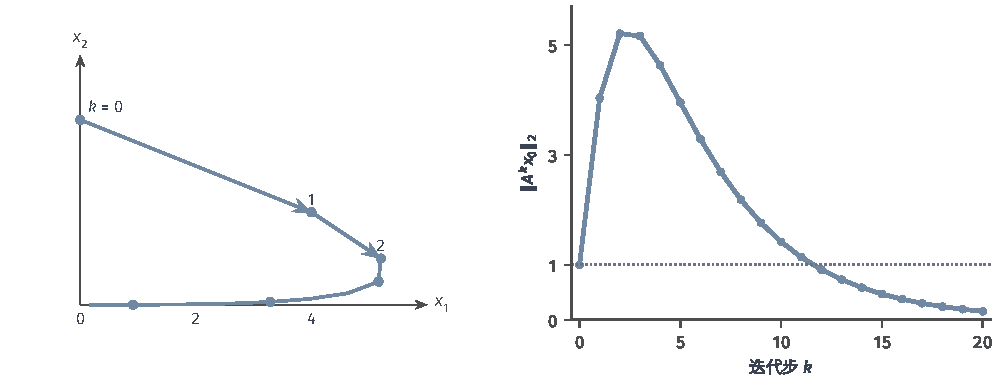
\includegraphics[width=169.0mm]{figures/00-shared/mathematical-preliminaries-upper/02-linear-spaces/matplotlib/ch06-transient-growth/figure.pdf}
  \caption{固定二维矩阵的反复作用。初值为$(0,1)^{\top}$，前两步的长度增加，
  此后回到原点；右图将长度与初始长度$1$比较。特征值$0.8$和$0.5$决定长期衰减，
  非正交特征方向间的相消则决定早期放大。两图使用同一个矩阵和同一组迭代点。}
  \label{fig:ch06-transient-growth}
\end{figure*}

一般地，设$\bm T$能用实可逆矩阵$\bm V$对角化，$\bm T=\bm V\bm\Lambda\bm V^{-1}$，$\bm\Lambda=\operatorname{diag}(\lambda_1,\ldots,\lambda_d)$为实对角矩阵。则$\bm T^k=\bm V\bm\Lambda^k\bm V^{-1}$；又
\[
 \lVert\bm\Lambda^k\bm x\rVert_2^2=\sum_i\lambda_i^{2k}x_i^2\leq\rho(\bm T)^{2k}\lVert\bm x\rVert_2^2 ,
\]
即$\lVert\bm\Lambda^k\rVert_2\leq\rho(\bm T)^k$。由次乘性，
\[
 \lVert\bm T^k\rVert_2\leq\lVert\bm V\rVert_2\lVert\bm V^{-1}\rVert_2\,\rho(\bm T)^k .
\]
因子$\lVert\bm V\rVert_2\lVert\bm V^{-1}\rVert_2$不小于$1$，因为$1=\lVert\bm V\bm V^{-1}\rVert_2\leq\lVert\bm V\rVert_2\lVert\bm V^{-1}\rVert_2$；它越大，这个上界允许的早期放大越强。

在示例~\ref{ex:ls-transient-growth}中取$\bm V=[\bm v_1\;\bm v_2]$，两条特征方向的夹角只有约$4.3^\circ$（示例~\ref{ex:ls-nonnormal-norm-radius}）。直接验证
\[
 \bm V=\begin{bmatrix}1&-40/3\\0&1\end{bmatrix},\qquad
 \bm V^{-1}=\begin{bmatrix}1&40/3\\0&1\end{bmatrix}.
\]
于是两个因子分别满足
\[
 \begin{aligned}
 \lVert\bm V\rVert_2&\geq\lVert\bm V\bm e_2\rVert_2=\lVert\bm v_2\rVert_2\approx13.37,\\
 \lVert\bm V^{-1}\rVert_2&\geq\lVert\bm V^{-1}\bm e_2\rVert_2\approx13.37 ,
 \end{aligned}
\]
乘积超过$178$。

贯穿例与示例~\ref{ex:ls-jordan-transient}则不可对角化。以贯穿例为例，它只有特征值$1/2$，而
\[
 \bm T-\tfrac12\bm I=\begin{bmatrix}0&1\\0&0\end{bmatrix}
\]
的零空间只是$\operatorname{span}\{\bm e_1\}$，凑不出两个线性无关的特征向量；两例的放大都来自式~\eqref{eq:ch06-jordan-power}中的多项式因子。

正规矩阵与此相反：第~\ref{sec:ls-general-square-spectrum}节证明了$\lVert\bm T^k\rVert_2=\rho(\bm T)^k$，每一步的最大放大倍数恰为谱半径。其中幂次取$1$得$\lVert\bm T\rVert_2=\rho(\bm T)$，于是每一步都有
\[
 \lVert\bm e_{j+1}\rVert_2\leq\lVert\bm T\rVert_2\lVert\bm e_j\rVert_2=\rho(\bm T)\lVert\bm e_j\rVert_2 ,
\]
所以$\rho(\bm T)<1$时误差的长度从第一步起就不增加。

所以，长期衰减、有限步内的最大放大和具体初始方向的表现要分别考察，不能只用谱半径估计中途的误差。

暂时放大说明谱半径不是单步倍率。它确切刻画的是矩阵幂的长期几何速率。
\begin{theorem}[Gelfand公式]
\label{thm:ls-gelfand-formula}
对实方阵$\bm T$与$d\times d$矩阵空间上的任意范数$\lVert\cdot\rVert$，
\begin{equation}
 \rho(\bm T)=\lim_{k\to\infty}\lVert\bm T^k\rVert^{1/k}.
 \label{eq:ls-gelfand-formula}
\end{equation}
若该范数还满足次乘性，则$\rho(\bm T)\leq\lVert\bm T\rVert$。
\end{theorem}
\begin{proof}
先在二范数中证明。上界：对任意$r>\rho(\bm T)$，由引理~\ref{lem:ls-power-geometric-bound}，
\[
 \lVert\bm T^k\rVert_2^{1/k}\leq C_r^{1/k}r ,
\]
而$C_r^{1/k}\to1$，所以$\limsup_k\lVert\bm T^k\rVert_2^{1/k}\leq r$。

下界：取模为$\rho(\bm T)$的特征值$\lambda$，重复定理~\ref{thm:ls-power-decay}必要性证明中的估计。若$\lambda$为实数，取单位特征向量$\bm v$，则$\lVert\bm T^k\rVert_2\geq\lVert\bm T^k\bm v\rVert_2=\rho(\bm T)^k$。若$\lambda$非实，同一证明中的$\bm u\neq\bm0$满足$\lVert\bm T^k\bm u\rVert_2\geq\rho(\bm T)^k/\lVert\bm L\rVert_2$，所以
\[
 \lVert\bm T^k\rVert_2\geq c\,\rho(\bm T)^k,\qquad c=\frac1{\lVert\bm L\rVert_2\lVert\bm u\rVert_2}>0 ,
\]
其中$c$与$k$无关。

两种情形都有$\lVert\bm T^k\rVert_2^{1/k}\geq c^{1/k}\rho(\bm T)$（实特征值时$c=1$），而$c^{1/k}\to1$，故$\liminf_k\lVert\bm T^k\rVert_2^{1/k}\geq\rho(\bm T)$。

合起来，对每个$r>\rho(\bm T)$，
\[
 \rho(\bm T)\leq\liminf_k\lVert\bm T^k\rVert_2^{1/k}\leq\limsup_k\lVert\bm T^k\rVert_2^{1/k}\leq r .
\]
令$r$趋于$\rho(\bm T)$，上下极限相等，极限存在且等于$\rho(\bm T)$。

再推广到任意范数。由有限维范数等价（定理~\ref{thm:ls-norm-equivalence}），存在与矩阵无关的常数$0<c_1\leq c_2$，使$c_1\lVert\bm B\rVert_2\leq\lVert\bm B\rVert\leq c_2\lVert\bm B\rVert_2$对所有$d$阶方阵成立。取$\bm B=\bm T^k$并开$k$次方，$c_1^{1/k}$与$c_2^{1/k}$都趋于$1$，由夹逼，$\lVert\bm T^k\rVert^{1/k}$与$\lVert\bm T^k\rVert_2^{1/k}$有相同的极限。

最后，若范数满足次乘性，则$\lVert\bm T^k\rVert\leq\lVert\bm T\rVert^k$，即$\lVert\bm T^k\rVert^{1/k}\leq\lVert\bm T\rVert$对每个$k$成立。令$k\to\infty$即得$\rho(\bm T)\leq\lVert\bm T\rVert$。
\end{proof}
最后一条说明，次乘性范数小于$1$必定使谱半径小于$1$，这正是本节开头的充分条件；贯穿例说明反过来不成立。

Gelfand公式说明，谱半径是矩阵幂最大放大倍数的长期几何平均。它不表示每条误差轨迹每一步都乘以同一个倍率：某些初值可能不含最慢衰减方向，非正规作用还可能在早期放大误差。

设$0<\rho(\bm T)<1$。若粗略用$\rho(\bm T)^m$估计$m$步后的长期倍率，由$\rho(\bm T)^m=1/10$得到缩小十倍的参考步数
\[
 m=\frac{1}{\log_{10}\bigl(1/\rho(\bm T)\bigr)} .
\]
例如$\rho=0.5$时约为$3.3$步，$\rho=0.99$时约为$229$步：谱半径接近零时每步都显著缩小误差，接近一时缩小十倍要上百步。

实际达到给定精度的步数还受常数、初始方向和暂时放大的影响。在示例~\ref{ex:ls-running-transient}中，参考步数约为$3.3$，但误差长度为
\[
 \lVert\bm e_k\rVert_2=2^{-k}\sqrt{4k^2+1} ,
\]
在$k=1,\ldots,7$时依次约为$1.118$、$1.031$、$0.760$、$0.504$、$0.314$、$0.188$、$0.110$，到$k=8$才第一次降到$0.1$以下（约为$0.063$），即要$8$步才缩小十倍。

精确解未知时还需要用可计算的量判断何时停止，这在第~\ref{chap:stationary-iterations}章联系残差讨论。

\section{误差传播与累积}
\label{sec:ls-accumulated-step-errors}

前面假设每一轮都精确执行。实际计算中，每轮可能引入新的误差，例如舍入，或者只近似地算出$\bm T\bm y_k$。把第$k$轮附加的误差记为$\bm\delta_k$，实际得到的序列满足
\[
 \bm y_{k+1}=\bm T\bm y_k+\bm c+\bm\delta_k .
\]
设$\rho(\bm T)<1$，$\bm x_\star$为定理~\ref{thm:ls-affine-common-limit}中的平衡，令$\bm e_k=\bm y_k-\bm x_\star$。与$\bm x_\star=\bm T\bm x_\star+\bm c$相减，得
\[
 \bm e_{k+1}=\bm T\bm e_k+\bm\delta_k .
\]
这与开头的更新形式相同，只是每轮的输入换成了$\bm\delta_k$，于是可以仿照有限展开分析。

\begin{theorem}[逐步误差的累积]
\label{thm:ls-accumulated-step-errors}
设$\rho(\bm T)<1$，$\bm y_k$与$\bm e_k$如上。
\begin{enumerate}
 \item 对每个$k\geq0$，
 \begin{equation}
  \bm e_k=\bm T^k\bm e_0+\sum_{j=0}^{k-1}\bm T^{k-1-j}\bm\delta_j .
  \label{eq:ls-accumulated-step-errors}
 \end{equation}
 \item 取一个向量范数及其诱导的矩阵范数，若$\lVert\bm T\rVert\leq q<1$且$\lVert\bm\delta_j\rVert\leq\delta$对所有$j$成立，则
 \begin{equation}
  \lVert\bm e_k\rVert\leq q^k\lVert\bm e_0\rVert+\delta\,\frac{1-q^k}{1-q},
  \label{eq:ls-noise-floor}
 \end{equation}
 从而$\limsup_{k\to\infty}\lVert\bm e_k\rVert\leq\delta/(1-q)$。
 \item 若只知道$\rho(\bm T)<1$，取$\rho(\bm T)<r<1$与引理~\ref{lem:ls-power-geometric-bound}中的常数$C_r$。若$\lVert\bm\delta_j\rVert_2\leq\delta$对所有$j$成立，则
 \begin{equation}
  \lVert\bm e_k\rVert_2\leq C_rr^k\lVert\bm e_0\rVert_2+C_r\delta\,\frac{1-r^k}{1-r}.
  \label{eq:ls-noise-floor-nonnormal}
 \end{equation}
\end{enumerate}
\end{theorem}
\begin{proof}
第一条对$k$归纳。$k=0$时和式为空。设等式对$k$成立，则
\[
\begin{aligned}
 \bm e_{k+1}&=\bm T\bm e_k+\bm\delta_k\\
 &=\bm T^{k+1}\bm e_0+\sum_{j=0}^{k-1}\bm T^{k-j}\bm\delta_j+\bm T^0\bm\delta_k ,
\end{aligned}
\]
末两项合起来是$\sum_{j=0}^{k}\bm T^{k-j}\bm\delta_j$，即$k+1$时的等式。

第二条。由三角不等式、诱导范数的界与次乘性，$\lVert\bm T^i\bm v\rVert\leq q^i\lVert\bm v\rVert$，所以
\[
\begin{aligned}
 \lVert\bm e_k\rVert&\leq q^k\lVert\bm e_0\rVert+\sum_{j=0}^{k-1}q^{k-1-j}\delta\\
 &=q^k\lVert\bm e_0\rVert+\delta\sum_{i=0}^{k-1}q^i ,
\end{aligned}
\]
末项的有限几何和等于$\delta(1-q^k)/(1-q)$，这就是式~\eqref{eq:ls-noise-floor}。右端随$k\to\infty$收敛到$\delta/(1-q)$，所以$\lVert\bm e_k\rVert$的上极限不超过它。

第三条。把第一条的展开取二范数，用$\lVert\bm T^i\rVert_2\leq C_rr^i$代替第二条中的$q^i$，同样求和即得。
\end{proof}
展开式中，第一项是初始误差的传播，按几何速度消失；和式中，$j$轮的附加误差再经过$k-1-j$次作用，较早的误差衰减得多，较近的误差几乎原样保留。

所以持续的附加误差不会随迭代消失，式~\eqref{eq:ls-noise-floor}右端随$k$增大趋于$\delta/(1-q)$，$q$越接近$1$，这个上界越大。

这是持续有界扰动下的最坏情形上界。它不是每条轨迹必然达到的误差下限：例如各轮误差都为零时，$\bm e_k=\bm T^k\bm e_0\to\bm0$，最终远小于$\delta/(1-q)$。

它也不保证误差存在极限。取$\bm T=\bm0$、$\bm c=\bm0$，则$\bm x_\star=\bm0$、$q=0$；再取单位向量$\bm u$与交替变号的附加误差$\bm\delta_k=(-1)^k\delta\bm u$，则对$k\geq1$，
\[
 \bm e_k=\bm\delta_{k-1}=(-1)^{k-1}\delta\bm u .
\]
误差的长度始终等于上界$\delta/(1-q)=\delta$，说明这个上界不能再改进，但$\bm e_k$来回翻转，没有极限。

第三条中两项都带着常数$C_r$：在非正规的$\bm T$下，即使每轮附加的误差很小，它们在被衰减之前也可能先被暂时放大，累积的上界因此按$C_r$倍增大。

有界误差留下一个不消失的误差水平。若附加误差本身逐渐变小，结论会改善，下面的定理分两种情形说明。为了只用一个范数书写，取$q$满足$\rho(\bm T)<q<1$；由引理~\ref{lem:ls-power-geometric-bound}，存在坐标范数$\lVert\cdot\rVert_*$使$\lVert\bm T\rVert_*\leq q$。若已经知道某个诱导范数满足$\lVert\bm T\rVert\leq q<1$，也可以直接用它。

\begin{theorem}[趋零与可求和的逐步误差]
\label{thm:recurrence-vanishing-summable-errors}
设$\rho(\bm T)<1$，$\bm e_k$如上，向量范数$\lVert\cdot\rVert$诱导的矩阵范数满足$\lVert\bm T\rVert\leq q<1$。
\begin{enumerate}
 \item 若$\bm\delta_j\to\bm0$，则$\bm e_k\to\bm0$。
 \item 若$\sum_{j=0}^\infty\lVert\bm\delta_j\rVert=D<\infty$，则对每个$k$，
 \begin{equation}
  \lVert\bm e_k\rVert\leq q^k\lVert\bm e_0\rVert+D ,
  \label{eq:ls-summable-step-errors}
 \end{equation}
 并且$\bm e_k\to\bm0$。
\end{enumerate}
\end{theorem}
\begin{proof}
两条都从定理~\ref{thm:ls-accumulated-step-errors}第一条的展开式出发，由三角不等式与$\lVert\bm T^i\bm v\rVert\leq q^i\lVert\bm v\rVert$，
\[
 \lVert\bm e_k\rVert\leq q^k\lVert\bm e_0\rVert+\sum_{j=0}^{k-1}q^{k-1-j}\lVert\bm\delta_j\rVert .
\]

第一条。任取$\varepsilon>0$，由$\bm\delta_j\to\bm0$，存在$J$使$j\geq J$时$\lVert\bm\delta_j\rVert\leq\varepsilon$。对$k>J$，把和式分成$j<J$与$j\geq J$两部分。前一部分中$k-1-j\geq k-J$，故它不超过$q^{k-J}\sum_{j<J}\lVert\bm\delta_j\rVert$；后一部分不超过
\[
 \varepsilon\sum_{i\geq0}q^i=\frac{\varepsilon}{1-q}.
\]
于是
\[
 \lVert\bm e_k\rVert\leq q^k\lVert\bm e_0\rVert+q^{k-J}\sum_{j<J}\lVert\bm\delta_j\rVert+\frac{\varepsilon}{1-q}.
\]
$J$固定后，前两项随$k\to\infty$趋于零，所以$\limsup_k\lVert\bm e_k\rVert\leq\varepsilon/(1-q)$。$\varepsilon$任意，故$\lVert\bm e_k\rVert\to0$，由有限维范数等价即$\bm e_k\to\bm0$。

第二条。$q^{k-1-j}\leq1$，所以和式不超过$\sum_j\lVert\bm\delta_j\rVert=D$，即得上界。收敛级数的通项趋于零，所以$\lVert\bm\delta_j\rVert\to0$，由第一条得$\bm e_k\to\bm0$。
\end{proof}

三种误差的差别在于每个误差被计入几次。有界误差每轮都重新加入，它们的贡献叠加成$\delta(1+q+q^2+\cdots)$，最终水平可达$\delta/(1-q)$，$q$越接近$1$越高。

趋零的误差最终也被消除，但误差不会比附加误差本身衰减得更快：例如$\bm T=\bm0$时$\bm e_{k+1}=\bm\delta_k$。

可求和的误差总量有限，每个误差进入后只会被衰减，所以累积误差不超过总量$D$，不再带因子$1/(1-q)$。

第~\ref{sec:ls-matrix-series-exponential}节末尾提出的逐步输入正是第一种情形的应用。若$\bm c_k\to\bm c$，令$\bm\delta_k=\bm c_k-\bm c$，则$\bm x_{k+1}=\bm T\bm x_k+\bm c+\bm\delta_k$，而$\bm\delta_k\to\bm0$，所以轨迹仍收敛到固定输入$\bm c$的平衡$(\bm I-\bm T)^{-1}\bm c$。

本章假设$\bm T$固定；具体算法如何产生附加误差、怎样选择更新规则和参数、何时停止计算，留给第~\ref{chap:stationary-iterations}章处理。

\FloatBarrier
\section{本章小结}
\label{sec:linear-recurrence-summary}

本章开头问：反复执行$\bm x_{k+1}=\bm T\bm x_k+\bm c$时，状态能否从任意初值趋于同一个平衡，接近得多快，每步的小误差又会累积到多大？展开递推得到$\bm x_k=\bm T^k\bm x_0+\sum_{j<k}\bm T^j\bm c$，三个问题都化为矩阵幂$\bm T^k$的行为。

初值的影响全部消失，当且仅当$\bm T^k\to\bm0$，当且仅当$\rho(\bm T)<1$。证明的关键是：对任意$r>\rho(\bm T)$，由实Schur形构造一个坐标范数，使$\bm T$在其中每步至多放大$r$倍，从而$\lVert\bm T^k\rVert_2\leq C_rr^k$。

范数小于$1$是便于检验的充分条件，但不是必要条件。$\rho(\bm T)=1$时，轨迹可能恒定、振荡、循环或无界增长，取决于是否缺少特征向量。

在同一条件$\rho(\bm T)<1$下，Neumann级数$\sum_j\bm T^j$收敛到$(\bm I-\bm T)^{-1}$，所有初值趋于同一个平衡$\bm x_\star=(\bm I-\bm T)^{-1}\bm c=\sum_j\bm T^j\bm c$，即历次输入经各自轮数传播后的总和。

$\bm I-\bm T$可逆只保证平衡唯一，不保证它吸引其他初值；输入随轮次变化时，$\rho(\bm T)<1$只保证初值影响消失，轨迹的去向还取决于输入序列。

谱半径决定长期的几何速度：Gelfand公式$\rho(\bm T)=\lim_k\lVert\bm T^k\rVert^{1/k}$，粗略地每$1/\log_{10}(1/\rho)$步缩小十倍。

它不是单步倍率。正规矩阵每步的放大恰为谱半径，误差从第一步起不增加；非正规矩阵的常数$C_r$可能远大于$1$，误差会先放大、再衰减，放大来自非正交特征方向的相消或Jordan块中的多项式因子。

每步附加的误差$\bm\delta_k$按$\bm T^{k-1-j}$传播后叠加。有界误差留下至多$\delta/(1-q)$的误差水平，它不随迭代消失；趋零的误差最终被消除；可求和的误差累积不超过其总量。非正规时这些上界还要乘以$C_r$。

因此，判断一个固定递推能否使用，要分别看三件事：谱半径是否小于一（能否收敛），常数与暂时放大有多大（中途误差会不会失控），每步误差属于哪一类（最终精度能达到多少）。第~\ref{chap:stationary-iterations}章由线性方程构造具体的更新矩阵，并结合残差决定何时停止；初值和输入随连续时间变化的线性系统，则在\BookChapterRef{chap:linear-differential-systems}{卷六“线性微分方程与系统”章}研究，那里矩阵幂换成矩阵指数。

